\documentclass[12pt, oneside]{book}
\pagestyle{plain}
\usepackage{tocloft}
\renewcommand{\cftchapleader}{\cftdotfill{\cftdotsep}}
\usepackage{pdfpages}
\usepackage{titlesec}

\setcounter{secnumdepth}{4}


\titleformat{\paragraph}
{\normalfont\normalsize\bfseries}{\theparagraph}{1em}{}
\titlespacing*{\paragraph}
{0pt}{3.25ex plus 1ex minus .2ex}{1.5ex plus .2ex}

\usepackage{optidef}
\usepackage{setspace}
\usepackage{amsfonts, amsthm,amsmath,amssymb,epsfig,graphicx,mathtools}
\usepackage{thmtools}
\usepackage{physics}
\usepackage{dsfont}
\usepackage{bbm}
\usepackage{bm}
\usepackage{mathtools}
\usepackage[square,numbers]{natbib}
\usepackage{graphicx}
\usepackage{svg}
\usepackage[pdftex,bookmarks=true,bookmarksopen=false,bookmarksnumbered=true,colorlinks=true,linkcolor=blue]{hyperref}
\usepackage[utf8]{inputenc}
\usepackage{float}
\usepackage{pdfpages}
\usepackage{bigints}
\usepackage{enumerate}
\usepackage{tikz}
\usepackage{tikz-qtree}
\usepackage{forest}
\usetikzlibrary{trees} % this is to allow the fork right path
\usepackage[autostyle]{csquotes}
\usepackage[ruled,vlined]{algorithm2e}
\newlength{\commentWidth}
\setlength{\commentWidth}{7cm}
\newcommand{\atcp}[1]{\tcp*[r]{\makebox[\commentWidth]{#1\hfill}}}
\usepackage{setspace}


\usepackage[british]{babel}
\theoremstyle{plain}
\newtheorem{theorem}{Theorem}[section]
\newtheorem{assumption}{Assumption}
\newtheorem{acknowledgment}{Acknowledgment}
\newtheorem{axiom}{Axiom}
\newtheorem{case}{Case}
\newtheorem{claim}{Claim}
\newtheorem{conclusion}{Conclusion} 
\newtheorem{condition}{Condition}
\newtheorem{conjecture}{Conjecture}
\newtheorem{corollary}{Corollary}[section]
\newtheorem{criterion}{Criterion}
\newtheorem{lemma}{Lemma}[section]
\newtheorem{proposition}{Proposition}[section]

\theoremstyle{definition}
\newtheorem{definition}{Definition}[section]

\newtheorem{example}{Example}[section]
\newtheorem{exercise}{Exercise}
\newtheorem{notation}{Notation}
\newtheorem{problem}{Problem}
\newtheorem{remark}{Remark}
\newtheorem{solution}{Solution}
\newtheorem{summary}{Summary}
\newenvironment{prf}[1][Proof]{\textbf{#1.} }{\qed}

%%%%%%%%%%%%%%%%%%%%%%%%%%%%%%%%%%%%%%%%%%%%%%%%%%%%%%%%%%%%
%                 TEX MACRO FILE, J.M. MACHADO
%                       DECEMBER 5, 2017
%%%%%%%%%%%%%%%%%%%%%%%%%%%%%%%%%%%%%%%%%%%%%%%%%%%%%%%%%%%%



\newcommand{\newpagec}{}

\newcommand{\XXX}[1]{{\bf \; XXX #1}}
%\newcommand{\XXX}[1]{}

% %%%--------------------------------------

\def\densesubset{\mathop{\stackrel{\rightharpoonup}{\subset}}}

\def\dd{{\rm d}}
\newcommand{\ddt}{\frac{\rm d}{{\rm d} t} }
\newcommand{\dotex}[1]{{\frac{\displaystyle d #1}{\displaystyle dt}}}
\newcommand{\ideal}[1]{\langle #1 \rangle}

%%%%%%%%%%%%%%%%%%%%%%%%%%%%%%%%%%%%%%% EMPHAZISE, ETC 
\newcommand{\new}[1]{{\em #1}}
\newcommand{\newd}[2]{{\em #1}\index{#2}}
%\newcommand{\prob}[1]{{\em #1}\index{#1}}
\newcommand{\mrm}[1]{\text{\rm #1}}
%%%%%%%%%%%%%%%%%%%%%%%%%%%%%%%%%%%%% GRAPHES 
% \newcommand{\arc}[2]{(#1,#2)}
\def\arcset{{\mathcal A}}
\def\nodeset{{\mathcal N}}
\def\incid{{M}}
\newcommand{\edge}[2]{\{#1,#2\}}
% %%%%%%%%%%%%%%%%%%%%%%%%%%%%%%%%%%%%% DIVERS S. Gaubert

\newcommand{\ov}[1]{\overline{#1}}
\newcommand{\arcm}[2]{#1#2}

\newcommand{\diagdots}{_{^{\big\cdot}\cdot _{\big\cdot}}}

\newcommand{\transp}{^\top}
\newcommand{\wglobal}[1]{\typeout{warning: #1 global definition}#1}
\newcommand{\promis}{\typeout{warning: verifier que c est fait}}
\newcommand{\ext}{\operatorname{extr}}
\newcommand{\co}{\operatorname{co}}
\newcommand{\cob}{\operatorname{\overline{co}}}
\newcommand{\set}[2]{\{#1\mid\,#2\}}

\newenvironment{sgdelicat}{\small}{}
\newenvironment{sgremarque}{\begin{remark}}{\hfill $\bullet$\end{remark}}

\def\weight(#1,#2){c_{#1,#2}}
%%%%%%%%%%%%%%%%%%%%%%%%%%%%%%%%%%%%% DIVERS RO
\def\Kh{\hat{K}} 
\def\Eb{\bar{E}}
\def\Adj{{\rm Adj}}
\def\Adjc{{\rm Adjc}}
\def\deg{{\rm deg}}
\def\red{{\rm red}}
\def\ra{{\rm ra}}
\def\ovdeg{{\overline{\rm deg}}}
\def\degu{\underline{\rm deg}}
\def\Mh {{\hat M}}
%%%%%%%%%%%%%%%%%%%%%%%%%%% Prog Dyn
\def\qbo {{\bf q}}
\def\ubo {{\bf u}}
\def\ybo {{\bf y}}
\def\uv {{\underline v}}


% \newcommand{\norm}[1]{\left\lVert#1\right\rVert}
\newcommand{\inner}[1]{\left\langle#1\right\rangle}
% \newcommand{\partialderivative}[2]{\frac{\partial#1}{\partial#2}}
%\newcommand{\thm}{th\'eor\`eme }
\newcommand{\un}{un }
% MATHS
\newcommand\meas{\mathop{\rm meas}}
%\renewcommand\rank{\mathop{\rm rang}}
\newcommand\mathpi{\mathop\Pi}

% MATHS
  \renewcommand\meas{\mathop{\rm meas}}  
%  \renewcommand\rank{\mathop{\rm rank}}
%} \fi
%%%%%%%%%%%%%%%%%%%%%%%%%%%%%%%%%%%%%%%%%%%%%%%%%%%%%%%%%%

% % \if { 
% % \renewcommand{\chapterl}[1]{\chapter{\LARGE \bf {#1}}\vspace{-40mm}}
% % \renewcommand{\sectionl}[1]{\section{\LARGE \bf {#1}}}
% % \renewcommand{\subsectionl}[1]{\subsection{\LARGE \bf {#1}}}
% % \renewcommand{\subsubsectionl}[1]{\subsubsection{\Large \bf {#1}}}
% % \renewcommand{\paragraphl}[1]{\paragraph{\LARGE \bf {#1}}}
% % \renewcommand{\subparagraphl}[1]{\subparagraph{\LARGE \bf {#1}}}

% % \renewcommand{\captionl}[1]{\caption{\LARGE \bf {#1}}}

% % \renewcommand{\Largel}{\Large}}{{\caption}}
% % } \fi

% %%%%%%%%%%%%%%%%%%%%%%%%%%%%%%%%%%%%%%%%%%%%%%%%%%%%%%%%%%%%
\newcommand\findem{\hfill{$\blacksquare$}\medskip}
% %%%%%%%%%%%%%%%%%%%%%%%%%%%%%%%%%%%%%%%%%%%%%%%%%%%%%%%%%%%%


% %%%%%%%%%%%%%%%%%%%%%%%%%% PROOFS %%%%%%%%%%%%%%%%%%%%%%%%%%%%
% \newcommand{\debdem}{\begin{proof}} \def\findem{\end{proof}}

%%% \newenvironment{proof}{{\noindent \bf D\'emonstration.}\quad}{\hfill{$\blacksquare$}\medskip}
\newenvironment{proofdu}[1]{{\noindent \bf D\'emonstration #1.}\quad}{\hfill{$\blacksquare$}\medskip}

%%% \newcommand{\qed}{\findem}
%%%%%%%%%%%%%%%%%%%%%%%%%%%%%%%%%%%%%%%%%%%%%%%%%%%%%%%%%%%%

\newcommand\ML{{\rm M}}

% %%%%%%%%%%%%%%%%%%%%%%%%%%%%%%%% CHECK CHECH %%%%%%%%%%%%%%%%%%%%%%%%
\def\ack{\check{a}}
\def\bck{\check{b}}
\def\cck{\check{c}}
\def\dck{\check{d}}
\def\eck{\check{e}}
\def\fck{\check{f}}
\def\gck{\check{g}}
\def\hck{\check{h}}
\def\ick{\check{i}}
\def\jck{\check{j}}
\def\kck{\check{k}}
\def\lck{\check{l}}
\def\mck{\check{m}}
\def\nck{\check{n}}
\def\ock{\check{o}}
\def\pck{\check{p}}
\def\qck{\check{q}}
\def\rck{\check{r}}
\def\sck{\check{s}}
\def\tck{\check{t}}
\def\uck{\check{u}}
\def\vck{\check{v}}
\def\wck{\check{w}}
\def\xck{\check{x}}
\def\yck{\check{y}}
\def\zck{\check{z}}

% %%%%%%%%%%%%%%%%%%%%%%%%%%%%%%%% HAT %%%%%%%%%%%%%%%%%%%%%%%%
\def\ah{\hat{a}}
\def\bh{\hat{b}}
\def\ch{\hat{c}}
\def\dh{\hat{d}}
\def\eh{\hat{e}}
\def\fh{\hat{f}}
\def\gh{\hat{g}}
\def\hh{\hat{h}}
\def\ih{\hat{i}}
\def\jh{\hat{j}}
\def\kh{\hat{k}}
\def\lh{\hat{l}}
\def\mh{\hat{m}}
\def\nh{\hat{n}}
\def\oh{\hat{o}}
\def\ph{\hat{p}}
\def\qh{\hat{q}}
\def\rh{\hat{r}}
\def\sh{\hat{s}}
\def\th{\hat{t}}
\newcommand\tth{\hat{t}}
\def\uh{\hat{u}}
\def\vh{\hat{v}}
\def\wh{\hat{w}}
\def\xh{\hat{x}}
\def\yh{\hat{y}}
\def\zh{\hat{z}}
%%%%%%%%%%%%%% UPPERCASE HAT %%%%%%%%
\newcommand\Ah{\hat{A}}
\newcommand\Bh{\hat{B}}
\newcommand\Ch{\hat{C}}
\newcommand\Dh{\hat{D}}
\newcommand\Eh{\hat{E}}
\newcommand\Hh{\hat{H}}
\newcommand\Ih{\hat{I}}
\newcommand\Lh{\hat{L}}
\newcommand\Ph{\hat{P}}
\newcommand\Qh{\hat{Q}}
\newcommand\Th{\hat{T}}
\newcommand\Uh{\hat{U}}
\newcommand\Vh{\hat{V}}
\newcommand\Wh{\hat{W}}

% THESE LINES CAUSE ERROR - DAVI
% %%%%%%%%%%%%%%%%%%%%%%%%%%%%%%%% BAR %%%%%%%%
% \def\ab{\bar{a}}
% \def\bb{\bar{b}}
% \def\cb{\bar{c}}
% \def\db{\bar{d}}
% \def\eb{\bar{e}}
% \def\fb{\bar{f}}
% \def\gb{\bar{g}}
% \def\hb{\bar{h}}
% \def\ib{\bar{i}}
% \def\jb{\bar{j}}
% \def\kb{\bar{k}}
% \def\lb{\bar{l}}
% \def\mb{\bar{m}}
% \def\nb{\bar{n}}
% \def\ob{\bar{o}}
% \def\pb{\bar{p}}
% \def\qb{\bar{q}}
% \def\rb{\bar{r}}
% \def\sb{\bar{s}}
% \def\tb{\bar{t}}
% \def\ub{\bar{u}}
% \def\vb{\bar{v}}
% \def\wb{\bar{w}}
% \def\xb{\bar{x}}
% \def\yb{\bar{y}}
% \def\zb{\bar{z}} 

% %%%%%%%%%%%%%%%%%%%%%%%%%%%%%%%% UPPERCASE BAR %%%%%%%%%%%%%%
% \def\Ab{\bar{A}}
% \def\Bb{\bar{B}}
% \def\Cb{\bar{C}}
% \def\Db{\bar{D}}
% \def\Eb{\bar{E}}
% \def\Fb{\bar{F}}
% \def\Gb{\bar{G}}
% \def\Hb{\bar{H}}
% \def\Ib{\bar{I}}
% \def\Jb{\bar{J}}
% \def\Kb{\bar{K}}
% \def\Lb{\bar{L}}
% \def\Mb{\bar{M}}
% \def\Nb{\bar{N}}
% \def\Ob{\bar{O}}
% \def\Pb{\bar{P}}
% \def\Qb{\bar{Q}}
% \def\Rb{\bar{R}}
% \def\Sb{\bar{S}}
% \def\Tb{\bar{T}}
% \def\Ub{\bar{U}}
% \def\Vb{\bar{V}}
% \def\Wb{\bar{W}}
% \def\Xb{\bar{X}}
% \def\Yb{\bar{Y}}
% \def\Zb{\bar{Z}}

% \def\Cbar{\bar{C}}
% \def\Tbar{\bar{T}}
% \def\Zbar{\bar{Z}}
%%%%%%%%%%%%%%%%%%%%%%%%%%%%%%%% TILDE %%%%%%%%%%%%%%%%%%%%%%%%

\def\at{\tilde{a}}
\def\bt{\tilde{b}}
\def\ct{\tilde{c}}
\def\dt{\tilde{d}}
\def\et{\tilde{e}}
\def\ft{\tilde{f}}
\def\gt{\tilde{g}}
\def\hit{\tilde{h}}
\def\iit{\tilde{i}}
\def\jt{\tilde{j}}
\def\kt{\tilde{k}}
\def\lt{\tilde{l}}
\def\mt{\tilde{m}}
\def\nt{\tilde{n}}
\def\ot{\tilde{o}}
\def\pt{\tilde{p}}
\def\qt{\tilde{q}}
\def\rt{\tilde{r}}
\def\st{\tilde{s}}
\def\tt{\tilde{t}}
\def\ut{\tilde{u}}
\def\vt{\tilde{v}}
\def\wt{\tilde{w}}
\def\xt{\tilde{x}}
\def\yt{\tilde{y}}
\def\zt{\tilde{z}}
%%%%%%%%%%%%%%%%%%%%%%%%%%%%%%%% UPPERCASE TILDE %%%%%%%%%%%%%%%%
\def\At{\tilde{A}} 
\def\Lt{\tilde{L}} 
\def\Pt{\tilde{P}} 
\def\Qt{\tilde{Q}} 
\def\Rt{\tilde{R}} 
\def\St{\tilde{S}} 
\def\Vt{\tilde{V}} 
\def\Wt{\tilde{W}} 
\def\Xt{\tilde{X}} 
\def\Yt{\tilde{Y}} 
\def\Zt{\tilde{Z}} 


\def\tA{\tilde{A}} 
\def\tL{\tilde{L}} 
\def\tS{\tilde{S}} 
\def\tV{\tilde{V}} 
\def\tW{\tilde{W}} 
\def\tX{\tilde{X}} 
\def\tY{\tilde{Y}} 
\def\tZ{\tilde{Z}} 


%%%%%%%%%%%%%%%%%%%%%%%%%%%%%%%% BOLDFACE %%%%%%%%%%%%%%%%%%%%%%%
\def\ebf { {\bf e}}  
\def\fbf { {\bf f}}  
\def\gbf { {\bf g}}  
\def\hbf { {\bf h}}  
\def\mbf { {\bf m}}  
\def\pbf { {\bf p}}  
\def\qbf { {\bf q}}  
\def\rbf { {\bf r}}  
\def\sbf { {\bf s}}  
\def\ubf { {\bf u}}  
\def\vbf { {\bf v}}  
\def\wbf { {\bf w}}  
\def\xbf { {\bf x}}  
\def\ybf { {\bf y}}  
\def\zbf { {\bf z}}  
%%%%%%%%%%%%%%%%%%%%%%%%%%%%%%%% HAT BOLDFACE %%%%%%%%%%%%%%%%%%%%%%%
\def\hebf {\hat {{\bf e} }}  
\def\hfbf {\hat {{\bf f} }}  
\def\hgbf {\hat {{\bf g} }}  
\def\hhbf {\hat {{\bf h} }}  
\def\hpbf {\hat {{\bf p} }}
\def\hqbf {\hat {{\bf q} }}  
\def\hrbf {\hat {{\bf r} }}  
\def\hsbf {\hat {{\bf s} }}  
\def\hubf {\hat {{\bf u} }}  
\def\hvbf {\hat {{\bf v} }}  
\def\hwbf {\hat {{\bf w} }}  
\def\hxbf {\hat {{\bf x} }}  
\def\hybf {\hat {{\bf y} }}  
\def\hzbf {\hat {{\bf z} }}  
%%%%%%%%%%%%%%%%%%%%%%%%%%%%%%%% BAR BOLDFACE %%%%%%%%%%%%%%%%%%%%%%%
\def\bebf {\bar {{\bf e} }}  
\def\bfbf {\bar {{\bf f} }}  
\def\bgbf {\bar {{\bf g} }}  
\def\bhbf {\bar {{\bf h} }}  
\def\bpbf {\bar {{\bf p} }}
\def\bqbf {\bar {{\bf q} }}  
\def\brbf {\bar {{\bf r} }}  
\def\bsbf {\bar {{\bf s} }}  
\def\bubf {\bar {{\bf u} }}  
\def\bvbf {\bar {{\bf v} }}  
\def\bwbf {\bar {{\bf w} }}  
\def\bxbf {\bar {{\bf x} }}  
\def\bybf {\bar {{\bf y} }}  
\def\bzbf {\bar {{\bf z} }}  
%%%%%%%%%%%%%%%%%%%%%%%%%%%%%%%% TILDE BOLDFACE %%%%%%%%%%%%%%%%%%%%%%%
\def\tebf {\tilde {{\bf e} }}  
\def\tfbf {\tilde {{\bf f} }}  
\def\tgbf {\tilde {{\bf g} }}  
\def\thbf {\tilde {{\bf h} }}  
\def\tpbf {\tilde {{\bf p} }}
\def\tqbf {\tilde {{\bf q} }}  
\def\trbf {\tilde {{\bf r} }}  
\def\tsbf {\tilde {{\bf s} }}  
\def\tubf {\tilde {{\bf u} }}  
\def\tvbf {\tilde {{\bf v} }}  
\def\twbf {\tilde {{\bf w} }}  
\def\txbf {\tilde {{\bf x} }}  
\def\tybf {\tilde {{\bf y} }}  
\def\tzbf {\tilde {{\bf z} }}  

%%%%%%%%%%%%%%%%%%%%%%%%%%%%%%%% CAL + TILDE  %%%%%%%%%%%%%%%%%%%%%
\def\calat{{\tilde {\mathcal A}}}

%%%%%%%%%%%%%%%%%%%%%%%%%%%%%%%% CAL %%%%%%%%%%%%%%%%%%%%%%%%%%%%
\def\cala{{\mathcal  A}}
\def\calb{{\mathcal B}}
\def\calc{{\mathcal C}}
\def\cald{{\mathcal D}}
\def\cale{{\mathcal E}}
\def\calf{{\mathcal F}}
\def\calg{{\mathcal G}}
\def\calh{{\mathcal H}}
\def\cali{{\mathcal I}}
\def\calj{{\mathcal J}}
\def\calk{{\mathcal K}}
\def\call{{\mathcal L}}
\def\calm{{\mathcal M}}
\def\caln{{\mathcal N}}
\def\calo{{\mathcal O}}
\def\calp{{\mathcal P}}
\def\calq{{\mathcal Q}}
\def\calr{{\mathcal R}}
\def\cals{{\mathcal S}}
\def\calt{{\mathcal T}}
\def\calu{{\mathcal U}}
\def\calv{{\mathcal V}}
\def\calw{{\mathcal W}}
\def\calx{{\mathcal X}}
\def\caly{{\mathcal Y}}
\def\calz{{\mathcal Z}}
%%%%%%%%%%%%%%%%%%%%%%%%%%%% OTHER CAL %%%%%%%%%%%%%%%%%%%%%%%%%%
\def\cA{{\mathcal A}}
\def\cF{{\mathcal F}}
\def\cL{{\mathcal L}}
\def\cP{{\mathcal P}}
\def\cQ{{\mathcal Q}}
\def\cR{{\mathcal R}}
\def\cV{{\mathcal V}}
\def\cW{{\mathcal W}}
\def\cO{{\mathcal O}}

\def\cPt{\widetilde{\cal P}}
%%%%%%%%%%%%%%%%%%%%%%%%%%%%%%%% MATHCAL %%%%%%%%%%%%%%%%%%%%%%%%
\def\A{\mathcal{A}}
\def\B{\mathcal{B}}
\def\C{\mathcal{C}}
\def\D{\mathcal{D}}
\def\E{\mathcal{E}}
\def\F{\mathcal{F}}
\def\G{\mathcal{G}}
\def\H{\mathcal{H}}
\def\I{\mathcal{I}}
\def\J{\mathcal{J}}
\def\K{\mathcal{K}}
\def\L{\mathcal{L}}
\def\M{\mathcal{M}}
\def\N{\mathcal{N}}
\def\P{\mathcal{P}}
\def\Q{\mathcal{Q}}
\def\R{\mathcal{R}}
\def\SS{\mathcal{S}}
\def\T{\mathcal{T}}
\def\U{\mathcal{U}}
\def\V{\mathcal{V}}
\def\W{\mathcal{W}}
\def\X{\mathcal{X}}
\def\Y{\mathcal{Y}}
\def\Z{\mathcal{Z}}
%%%%%%%%%%%%%%%%%%%%%%%%%%%% AUTRES MATHCAL %%%%%%%%%%%%%%%%%%
\newcommand{\sB}{\mathcal{B}}
\newcommand{\sC}{\mathcal{C}}
\newcommand{\sE}{\mathcal{E}}
\newcommand{\sL}{\mathcal{L}}
\newcommand{\sS}{\mathcal{S}}
\newcommand{\sT}{\mathcal{T}}
\newcommand{\sV}{\mathcal{V}}
%%%%%%%%%%%%%%%%%%%%%%% OVERLINE  MATHCAL  %%%%%%%%%%%%%%%%%%%%%%%%
\newcommand{\Hbc}{\overline{\mathcal H}}


%%%%%%%%%%%%%%%%%%%%%%% OVERLINE   %%%%%%%%%%%%%%%%%%%%%%%%
\def\HH{\overline{\bf H}}


\newcommand{\Xbo}{\overline{X}}
\newcommand{\Ybo}{\overline{ Y}}

%%%%%%%%%%%%%%%%%%%%%%% UNDERLINE %%%%%%%%%%%%%%%%%%%%%%%%
\def\au{\underline{a}}
\def\xu{\underline{x}}
%
\def\uV{\underline{V}}

%%%%%%%%%%%%%%%%%%%%%%% GREEKS %%%%%%%%%%%%%%%%%%%%%%%%
\def\eps{\varepsilon}
\def\Om{{\Omega}}
\def\Omb{{\Omegab}}
\def\om{{\omega}}
\def\ml{\lambda}
%%%%%%%%%%%%%%%%%%%%%%% GREEK HATS %%%%%%%%%%%%%%%
\def\alphah{\hat{\alpha}}
\def\betah{\hat{\beta}}
\def\ellh{\hat{\ell}}
\def\etah{\hat{\eta}}
\def\gamh{\hat{\gamma}}
\def\kappah{\hat{\kappa}}
\def\mlh{\hat{\lambda}}
\def\lambdah{\hat{\lambda}}
\def\Lambdah{\hat{\Lambda}}
\def\muh{\hat{\mu}}
\def\nuh{\hat{\nu}}
\def\pih{{\hat\pi}}
\def\Phih{{\hat\Phi}}
\def\Phih{{\hat\Phi}}
\def\psih{{\hat\psi}}
\def\Psih{{\hat\Psi}}
\def\Psih{{\hat\Psi}}
\def\rhoh{{\hat\rho}}
\def\sigmah{{\hat\sigma}}
\def\tauh{{\hat\tau}}
\def\thetah{{\hat\theta}}
\def\xih{{\hat\xi}}

%%%%%%%%%%%%%%%%%%%%%%% GREEK BARS %%%%%%%%%%%%%%%
\def\alphab{\bar{\alpha}}
\def\betab{\bar{\beta}}
\def\chib{\bar{\chi}}
\def\gammab{\bar{\gamma}}
\def\deltab{\bar{\delta}}
\def\ellb{\bar{\ell}}
\def\epsb{\bar{\varepsilon}}
\def\etab{\bar{\eta}}
\def\kappab{\bar{\kappa}}
\def\mlb{\bar{\lambda}}
\def\lambdab{\bar{\lambda}}
\def\Lambdab{\bar{\Lambda}}
\def\mub{\bar{\mu}}
\def\nub{\bar{\nu}}
\def\pib{{\bar\pi}}
\def\Phib{{\bar\Phi}}
\def\phib{{\bar\phi}}
\def\psib{{\bar\psi}}
\def\Psib{{\bar\Psi}}
\def\Psih{{\hat\Psi}}
\def\sigmab{{\bar\sigma}}
\def\taub{{\bar\tau}}
\def\thetab{{\bar\theta}}
\def\varphib{{\bar\varphi}}
\def\xib{{\bar\xi}}
\def\zetab{{\bar\zeta}}

%%%%%%%%%%%%%%%%%%%%%%% GREEK TILDE %%%%%%%%%%%%%%%
\def\alphat{\tilde{\alpha}}
\def\betat{\tilde{\beta}}
\def\ellt{\tilde{\ell}}
\def\etat{\tilde{\eta}}
\def\kappat{\tilde{\kappa}}
\def\mlt{\tilde{\lambda}}
\def\lambdat{\tilde{\lambda}}
\def\Lambdat{\tilde{\Lambda}}
\def\mut{\tilde{\mu}}
\def\nut{\tilde{\nu}}
\def\omt{\tilde{\omega}}
\def\Omt{\tilde{\Omega}}
\def\pit{{\tilde\pi}}
\def\Phit{{\tilde\Phi}}
\def\Phit{{\tilde\Phi}}
\def\psit{{\tilde\psi}}
\def\Psit{{\tilde\Psi}}
\def\Psih{{\hat\Psi}}
\def\sigmat{{\tilde\sigma}}
\def\taut{{\tilde\tau}}
\def\thetat{{\tilde\theta}}
\def\thetat{{\tilde\theta}}
\def\xit{{\tilde\xi}}
\def\varphit{{\tilde\varphi}}


%%%%%%%%%%%%%%%%%%GREEK BOLDFACE AND BAR BOLDFACE %%%%%%%%%%
\def\alphabf {\boldsymbol\alpha}
\def\balphabf {\bar{\boldsymbol\alpha}}
\def\betabf {\boldsymbol\beta}
\def\bbetabf {\bar{\boldsymbol\beta}}
\def\etabf {\boldsymbol\eta}
\def\betabf {\bar{\boldsymbol\eta}}
\def\mubf {\boldsymbol\mu}
\def\blambdabf {\bar{\boldsymbol\lambda}}
\def\bmubf {\bar{\boldsymbol\mu}}
\def\pibf {\boldsymbol\pi}
\def\bpibf {\bar{\boldsymbol\pi}}
\def\xibf {\boldsymbol\xi}
\def\bxibf {\bar{\boldsymbol\xi}}
\def\taubf {\boldsymbol\tau}

%%%%%%%%%%%%%%%%%%%%%%%% MATH OPERATORS %%%%%%%%%%%%%%%%
\def\1B{{\bf  1}}

\newcommand{\ceil}[1]{\lceil #1 \rceil}
\newcommand{\floor}[1]{\lfloor #1 \rfloor}

\def\densesubset{\mathop{\stackrel{\rightharpoonup}{\subset}}}

\def\ad{\mathop{\rm ad}}
\def\affhull{\mathop{\rm affhull}}
\def\argmin{\mathop{\rm argmin}}
\def\argmax{\mathop{\rm argmax}}
\def\cl{\mathop{\rm cl}}
\newcommand\Comp{\mathop{\rm Comp}}
\def\caffhull{\mathop{\rm \overline{affhull}}}
\def\cone{\mathop{\rm cone}}
\def\core{\mathop{\rm core}}
\newcommand\conebar{\mathop{\rm \overline{cone}}}
\def\conv{\mathop{\rm conv}}
\def\convbar{\mathop{\rm \overline{conv}}}
\def\deg{\mathop{\rm deg}}
\def\det{\mathop{\rm det}}
\def\dett{\mathop{\rm det}}
\def\diag{{\mathop{\rm diag}}}
\newcommand\diam{\mathop{\rm diam}}
\def\dist{\mathop{\rm dist}}
\def\ddiv{\mathop{\rm div}}
\def\dom{\mathop{{\rm dom}}}
% \def\epi{\mathop{\text{\'epi}}}
\def\epi{\mathop{\text{epi}}}
\newcommand{\ess}{\mathop{\rm ess}}
\def\essinf{\mathop{\rm essinf}}
\def\essup{\mathop{\rm esssup}}
\def\esssup{\mathop{\rm esssup}}
\def\intt{\mathop{\rm int}}
\def\inv{\mathop{\rm inv}}
\def\isom{\mathop{\rm Isom}}
\def\lin{\mathop{\rm lin}}
\newcommand\Jac{{\mathop{\rm Jac}}}
\newcommand\Lip{\mathop{\rm Lip}}
\newcommand\snorm{\|}
\newcommand\lnlt{\mathop{\rm lnlt}}
% \newcommand\psicirc{{\stackrel \circ \psi}}
\newcommand\psicirc{ \psi}
\def\range{\mathop{\rm Im}}
\def\rec{\mathop{\rm rec}}
\def\ri{\mathop{\rm rint}}
\def\rint{\mathop{\rm rint}}
\def\sign{\mathop{\rm sign}}
\def\supp{\mathop{\rm supp}}
\def\trace{\mathop{\rm trace}}
\def\val{\mathop{\rm val}}
\def\var{\mathop{\rm var}}
\def\width{\mathop{{\rm width}}}
\def\View{\mathop{\rm View}}

\def\inf{\mathop{\rm inf}}
\def\Ker{\mathop{\rm Ker}}
\def\min{\mathop{\rm min}}
\def\max{\mathop{\rm max}}

\def\dw{\mathop{\delta w}}


\def\dPsi{\mathop{\delta \Psi}}

%%%%%%%%%%%%%%%% UNDERLINED AND OVERLINED LIMINF AND LIMSUP %%%
\def\liminfu{\mathop{\underline{\lim}}}
\def\limsupo{\mathop{\overline{\lim}}}
%%%%%%%%%%%%%%%%%%%%%%%%%%%%%%%% NUMBERS %%%%%%%%%%%%%%%%%%
\def\half{\mbox{$\frac{1}{2}$}}
\def\threeinv{\mbox{$\frac{1}{3}$}}
\def\fourinv{\mbox{$\frac{1}{4}$}}
\def\sixinv{\mbox{$\frac{1}{6}$}}
\def\1B{{\bf  1}}
\def\sbdeux#1#2{\mbox{\scriptsize$#1$}\atop\mbox{\scriptsize$#2$}}
\def\sbtrois#1#2#3{\mbox{\scriptsize$#1$}\atop\mbox{\scriptsize$#2$}\atop\mbox{\scriptsize$#3$}}
%%%%%%%%%%%%%%%%%%%%%%%%%%%%%%%%%  NUMBER SPACES  %%%%
\newcommand{\EE}{\mathbb{E}}
\newcommand{\FF}{\mathbb{F}}
\newcommand{\NN}{\mathbb{N}}
\newcommand{\RR}{\mathbb{R}}
\newcommand{\ZZ}{\mathbb{Z}}

%%%%%%%%%%%%%%%%%%%%%%%%%%%%%% OTHER MATHBB %%%%%%%%%%

\def\cC{\mathbb{C}}
\def\cN{\mathbb{N}}
\def\cP{\mathbb{P}}
\def\cQ{\mathbb{Q}}
\def\QQ{\mathbb{Q}}
\def\cR{\mathbb{R}}
\def\cZ{\mathbb{Z}}

%%%%%%%%%%%%%%%%%% OTHER TYPE OF MATHBB %%%%%%%%%%%
\newcommand{\bbC}{{\mathbb C}}
\newcommand{\bbH}{{\mathbb H}}
\newcommand{\bbI}{{\mathbb I}}
\newcommand{\bbK}{{\mathbb K}}
\newcommand{\bbN}{{\mathbb N}}
\newcommand{\bbO}{{\mathbb O}}
\newcommand{\bbP}{{\mathbb P}}
\newcommand{\bbQ}{{\mathbb Q}}
\newcommand{\bbR}{{\mathbb R}}
\newcommand{\bbS}{{\mathbb S}}
\newcommand{\bbZ}{{\mathbb Z}}


%%%%%%%%%%%%%%%%%%%%%%%%%%%% OTHER CAPS %%%%%%%%%%%
\newcommand{\gA}{\mathsf{A}}
\newcommand{\gE}{\mathsf{E}}
\newcommand{\gF}{\mathsf{F}}
\newcommand{\gG}{\mathsf{G}}
\newcommand{\gN}{\mathsf{N}}
\newcommand{\gT}{\mathsf{T}}
\newcommand{\gV}{\mathsf{V}}
\newcommand{\sG}{\mathcal{G}}
\newcommand{\sN}{\mathcal{N}}
\newcommand{\sA}{\mathcal{A}}


\newcommand{\cE}{I\!\!E}
% \newcommand{\cR}{I\!\! R} \newcommand{\cN}{I\!\!N}
%\newcommand{\cRbar}{\bar {I\!\! R}}
\newcommand{\cRbar}{\mathbb{\bar{R}}}
\newcommand{\rbar}{\overline{\mathbb{R}}}
\newcommand{\rbartosn}{\rbar^{_{\scriptstyle\sN}}}
%%%%%%%%%%%%%%%%%%%%%%%%%%%%%%%%  ENVIRONMENTS %%%%%%%%%%%%%%%%%%
\newcommand\be{\begin{equation}}
\newcommand\ee{\end{equation}}
\newcommand\ba{\begin{array}}
\newcommand\ea{\end{array}}
\newcommand{\bea}{\begin{eqnarray}}
\newcommand{\eea}{\end{eqnarray}}
\newcommand{\bean}{\begin{eqnarray*}}
\newcommand{\eean}{\end{eqnarray*}}

\newenvironment{paoplist}{\vspace{-1ex}\begin{list}{-}
{\itemsep 0mm \leftmargin 2mm \labelwidth 0mm}}
{\end{list} \vspace{-1ex}}

\newenvironment{myenumerate}{
\renewcommand{\theenumi}{\roman{enumi}}
\renewcommand{\labelenumi}{(\theenumi)}
\begin{enumerate}}{\end{enumerate}}
%%%%%%%%%%%%%%%%%%%%%%%%%%%%%%%%  SPACING %%%%%%%%%%%%%%%%%%
\newcommand{\noi}{\noindent}
\newcommand{\bs}{\bigskip}
\newcommand{\ms}{\medskip}
\newcommand{\msn}{{\bigskip \noindent}}
%%%%%%%%%%%%%%%%%%%%%%%%%%%%%%%%  MISC %%%%%%%%%%%%%%%%%%
%\newcommand{\refeq}[1]{(\ref{#1})}
%\newcommand{\eqref}[1]{(\ref{#1})}

\def\ATT{\marginpar{$\leftarrow$}}

\def\rar{\rightarrow}
\def\fmap{\rightarrow}

\def\ds{\displaystyle}
\def\disp{\displaystyle}

\def\La{\langle}
\def\la{\langle}
\def\ra{\rangle}
%%%%%%%%%%%%%%%%%%%%%%%%%% FIGURES %%%%%%%%%%%%%%%%%%%%%%%%%%%%%%%%%%

% \newcommand{\mypsfig}[3]
%            {\begin{figure}[hbtp]
%             \centerline{\input #1}
%             \caption{\rm{#2}} \label{#3}
%             \end{figure}}








%%% EOF
\def\TV{\text{TV}}

%%%%%%%%%% BOOK INFORMATION %%%%%%%%%%
\newcommand{\authorname}{Davi Barreira, João Miguel Machado}
\newcommand{\booktitle}{Introdução à Teoria de Transporte Ótimo}
\newcommand{\subtitle}{}
\newcommand{\publisher}{TBD}
\newcommand{\editionyear}{2021}
\newcommand{\isbn}{XYZ}   % replace this with your own ISBN
\title{\booktitle}
\author{\authorname}


\begin{document}
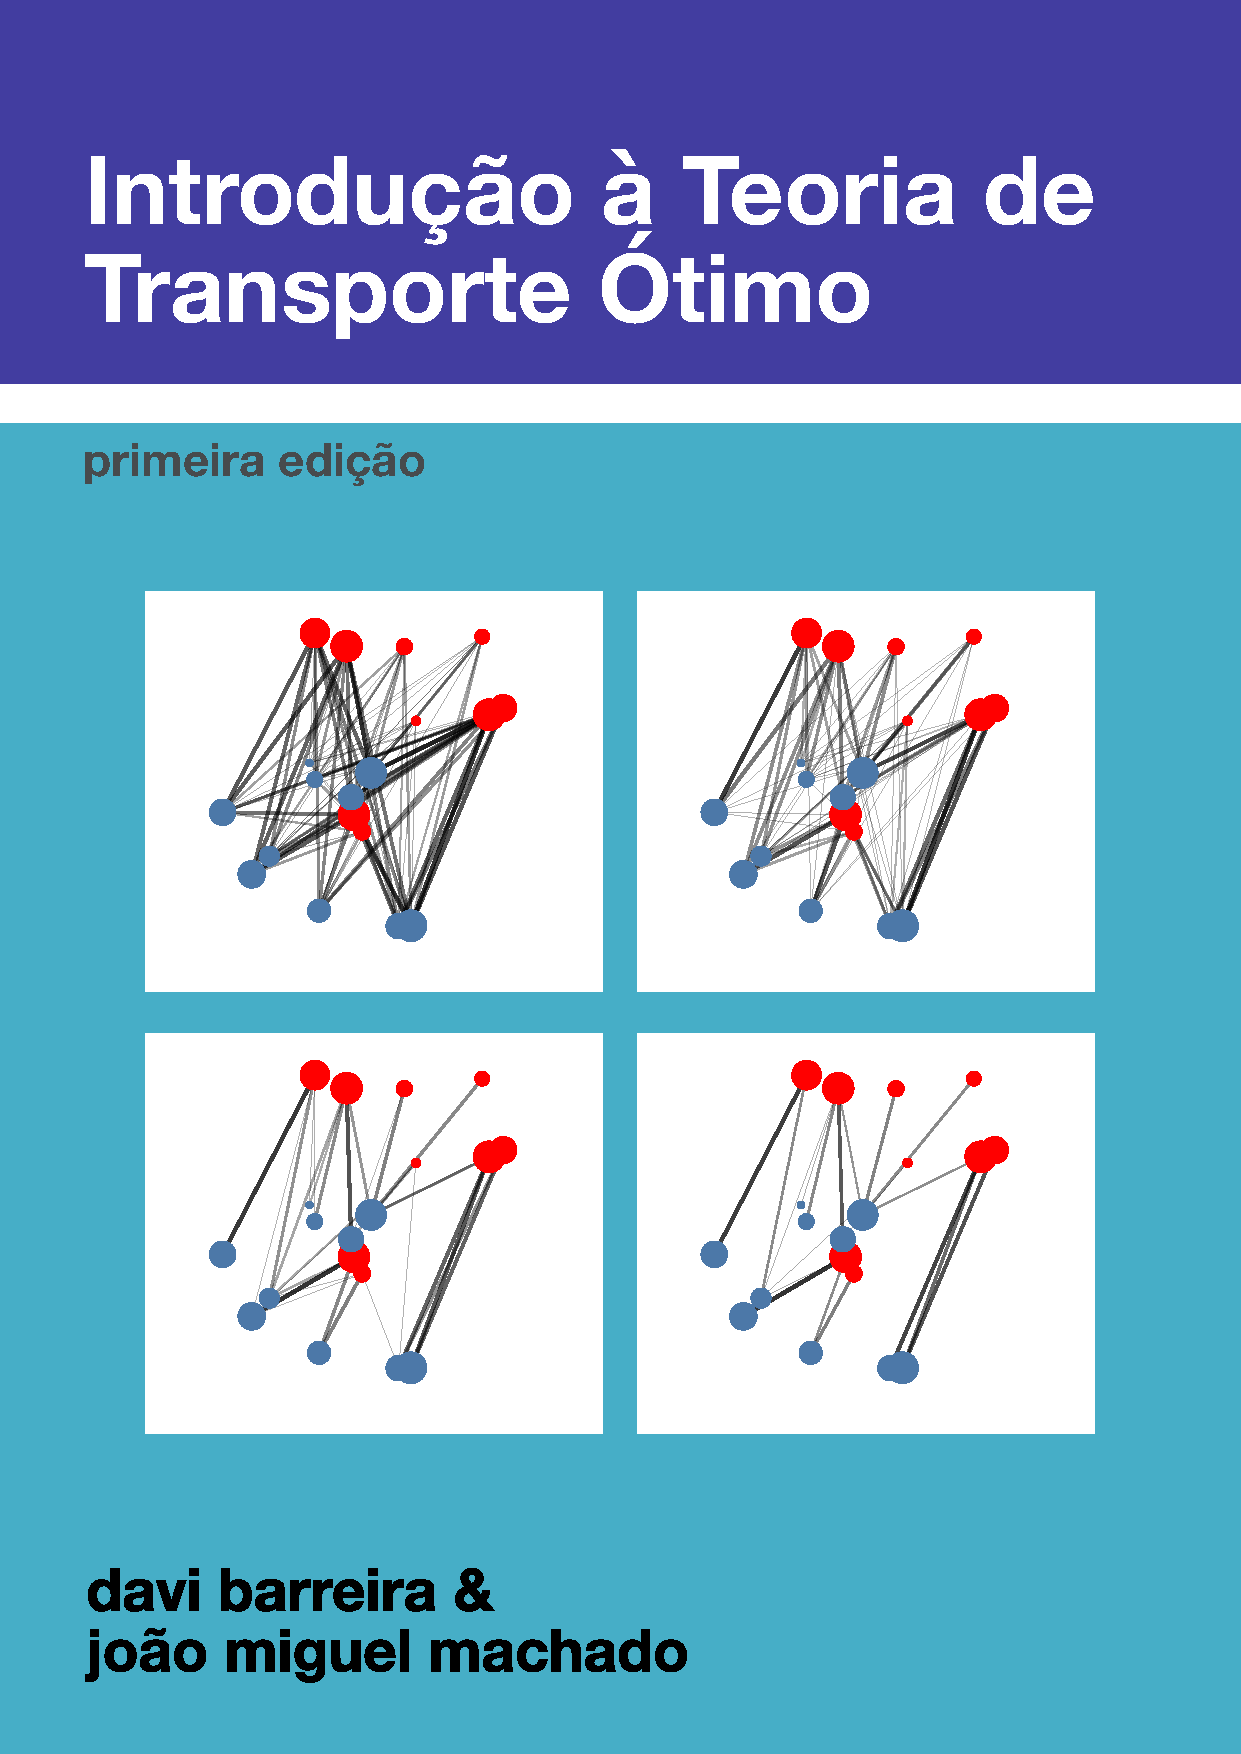
\includepdf{capa.pdf}
\frontmatter
% \pagestyle{empty}

% % Half title page
% {
% \centering

% ~

% \vspace{24pt}
% {\scshape\Huge \booktitle \par}
% }
% \cleardoublepage

% Title page
\begin{titlepage}
	\centering
	
	~
	
	\vspace{24pt}
	{\scshape\Huge \booktitle\par}
	\vspace{6pt}
	{\scshape\large \subtitle\par}
	\vspace{\stretch{1.25}}
	{\itshape\large by\par}
	\vspace{6pt}
	{\itshape\Large \authorname\par}
	\vspace{\stretch{6}}
	{\large \publisher\par}
\end{titlepage}

% Copyright page

{\small
\setlength{\parindent}{0em}\setlength{\parskip}{1em}

~

\vfill

Copyright \copyright{} 2021 \authorname

All rights reserved. No part of this publication may be reproduced, stored or transmitted in any form or by any means, electronic, mechanical, photocopying, recording, scanning, or otherwise without written permission from the publisher. It is illegal to copy this book, post it to a website, or distribute it by any other means without permission.

This novel is entirely a work of fiction. The names, characters and incidents portrayed in it are the work of the author’s imagination. Any resemblance to actual persons, living or dead, events or localities is entirely coincidental.

First edition, \editionyear{}

ISBN \isbn{}  % see main.tex

Published by \publisher{}
}

\newpage
\chapter*{Preface}
\addcontentsline{toc}{chapter}{Preface}

The field of Optimal Transport has grown quite substantially in recent years
\footnote{\citet{villani2008optimal} is roughly a thousand pages of theoretical results on OT.},
and going through the theory in order understand how it can be applied to real world problems can
be a challenging task for researchers not acquainted with the field.
Hence, we have filtered the main theoretical
results necessary for mathematically inclined researchers that are interested in learning
Optimal Transport.

These notes are mainly based on the book
``Optimal Transport for Applied Mathematicians'' by
\citet{santambrogio2015optimal}. We do not focus
on proving the measurability of the sets, functions and maps, although it can be indeed shown
that the ones presented here are indeed measurable.

As prerequisites to properly understand this text, we advise some knowledge of
Measure Theory and Functional Analysis. Although, we've tried to either prove or state
all the necessary results.




\newpage
\tableofcontents

\newpage
\chapter*{Notation}
\addcontentsline{toc}{chapter}{Notation}

The following symbols are used in the text without always recalling their meaning.

\begin{itemize}
	\item $\mathcal M(X), \mathcal M_+(X)$: Space of finite measures and finite positive measures on $X$, respectively.
	\item $\mathcal P(X), \mathcal P_p(X)$: Space of probability measures and space of probability
	measures with $p$th finite moment, respectively.
	\item $\mathbbm 1_A(x)$: Indicator function of set A, i.e. $\mathbbm 1_A(x)=1$ if $x \in A$ and 0 otherwise.
	\item $\mathbf 1_n$: $n$ dimensional vector of ones.
	\item $id$: Identity operator, i.e. $id(x)=x$.
	\item $\oplus$: For $\phi: X \to \mathbb R$, $\psi: Y \to \mathbb R$, then $(\phi \oplus \psi)(x,y) = \phi(x) + \psi(y)$.
	\item $\pi_X$: Projection operator on $X$, i.e. for $\pi_X : X \times Y \to X$, then $\pi_X(x,y)= x, \ \forall (x,y) \in X \times Y$.
	\item $\Pi(\mu,\nu)$: Coupling of measures $\mu$ and $\nu$.
	\item $\mathbb R_+$: Positive real number greater or equal than 0.
	\item $\mathbb{\overline R}$: Real numbers extended to include $+\infty$ and $-\infty$.
	\item $C(X)$: Set of functions $f: X \to \mathbb R$, where $f$ is continuous.
	\item $C_b(X)$: Set of functions $f: X \to \mathbb R$, where $f$ is continuous and bounded.
	\item $C_0(X)$: Set of functions $f: X \to \mathbb R$, where $f$ is continuous and goes to zero at infinity.
	\item $C_c(X)$: Set of functions $f: X \to \mathbb R$, where $f$ is continuous and has compact support.
	\item $\mu_n \rightharpoonup \mu$: Measure $\mu_n$ converges weakly to $\mu$.
	\item $OT_c(\mu,\nu)$: Optimal Transport cost between measures $\mu$ and $\nu$ for a ground cost function $c$.
	\item $OT_{c,\varepsilon}(\mu,\nu)$, $\overline{OT}_{c,\varepsilon}(\mu,\nu)$:
	Entropic Optimal Transport distance and the Entropic Optimal Transport cost
	between measures $\mu$ and $\nu$ for a ground cost function $c$, respectively.
	\item $W_p$, $W_{p,\varepsilon}$, $S_{c,\varepsilon}$, $SW$, $GW$: Wasserstein distance, Entropic Wasserstein distance,
	Sinkhorn divergence,
	Sliced-Wasserstein distance and Gromov-Wasserstein distance, respectively.
	\item $\mathrm{KL}$: Kullback-Leibler divergence.
\end{itemize}


\listoftheorems 
\listoffigures

\mainmatter
\newpage
\newpage
\chapter{Monge \& Kantorovich}

Let's start by providing some definitions that will be used throughout this section.
\begin{definition}
  Given $(\Omega,\mathcal F)$ where $\mathcal F$ is a $\sigma$-algebra,
  then, $\mu: \mathcal F \to [0,+\infty]$ is a measure if:
  \begin{enumerate}[i)]
    \item $\mu(\varnothing)=0$
    \item $(A_n)_{n\in \mathbb N} \subset \mathcal F$ with
          $A_j \cap A_i = \varnothing ,\ \forall i,j \in \mathbb N\implies
            \mu(\cup_{n \in \mathbb N}A_n) = \sum_{n \in \mathbb N}\mu(A_n)$
  \end{enumerate}
  We say that $\mu$ is a probability measure if besides the two
  properties above, we also have $\mu(\Omega) = 1$.
\end{definition}

\begin{definition}
  We call $\mathcal P(X)$ the space of probability measures defined
  on $(X,\mathcal F)$, where the $\sigma$-algebra $\mathcal F$
  is implicit and usually refers to the Borel $\sigma$-algebra.
\end{definition}

\begin{definition}(Pushforward)
  Let $(X,\mathcal F)$ and $(Y, \mathcal G)$ be measurable spaces, $T : X \to Y$ a measurable map
  and $\mu \in \mathcal P(X)$. We call $T_\# \mu$ the
  pushforward of $\mu$, where:
  \begin{equation}
    T_\#\mu(B) = \mu(T^{-1}(B)),\quad \forall B \in \mathcal G
  \end{equation}
\end{definition}

\begin{theorem}
  Let $T: X \to Y$ be a measurable map between
  $(X, \mathcal F, \mu)$ and $(Y, \mathcal G)$. Then,
  $T_\# \mu$ is a measure on $(Y, \mathcal G)$ and
  $\forall f$ measurable and integrable with respect to
  $T_\#\mu$ one has:
  \begin{equation}
    \int_Y f dT_\#\mu = \int_X f \circ T d\mu
  \end{equation}
  \label{thm:pushforward}
\end{theorem}
\begin{prf}
  Let $f_n$ be a simple positive measurable function. Hence
  \begin{equation*}
    \begin{multlined}
      f_n(y) = \sum^N_{i=0} a_i \mathbbm 1_{A_i}(y) \ \therefore
      \int_Y f_n \ dT_\# \mu =
      \sum^N_{i=0} a_i T_\# \mu(A_i) =
      \sum^N_{i=0} a_i \mu(T^{-1}(A_i) )
      \\
      (f_n\circ T)(x) =
      \sum^N_{i=0} a_i \mathbbm 1_{A_i}(T(x))=
      \sum^N_{i=0} a_i \mathbbm 1_{T^{-1}(A_i)}(x)
      \\
      \therefore
      \\
      \int_X f_n \circ T \ d\mu =
      \sum^N_{i=0} a_i \mu(T^{-1}(A_i) ) \\
    \end{multlined}
  \end{equation*}

  Hence, $\int_X f_n \circ T \ d\mu = \int_Y f_n \ dT_\# \mu$.

  Now, for a positive integrable measurable function
  $f$, there exists a sequence
  of positive simple functions such that $f_n \uparrow f$. Then,
  by the Monotone Convergence Theorem,
  \begin{align*}
    \int_Y f \ dT_\# \mu =
    \int_Y\lim_{n\to +\infty}  f_n \ dT_\# \mu & =
    \lim_{n\to +\infty} \int_Y f_n \ dT_\# \mu =                                                 \\
                                               & =\lim_{n\to +\infty}	\int_X f_n \circ T \ d\mu =
    \int_Y f \ dT_\# \mu
  \end{align*}

  If $f$ is non-positive, just use the same argument by splitting
  the negative and positive portions of the function.

\end{prf}

With these definitions, we can enunciate the so called Monge Problem,
which is known as the motivating problem that gave birth to the field
of Optimal Transport.

\begin{definition} (Monge Problem)
  Given two probability measures $\mu \in \mathcal P(X)$,
  $\nu \in \mathcal{P}(Y)$ and a cost function
  $c:X\times Y \to[0,+\infty]$, solve:
  \begin{flalign}
    (MP) &&
    \inf
    \left\{
    \int_{X} c(x,T(x))d\mu \quad : \quad
    T_\# \mu = \nu
    \right\}&&
  \end{flalign}

\end{definition}

In the Monge Problem, no mass can be split. Therefore, one can easily
come up with situations in which there is no solution to the problem,
as shown in \ref{fig:monge_map_example}. A viable solution $T$ to MP
is called a \textbf{Transport Map}.
\begin{figure}[H]
  \centering
  \def\svgscale{0.8}
  \includesvg[inkscapelatex=false]{Figures/monge_map_example.svg}
  \caption{Example of two Optimal Transport Problems. On the left, there exists an optimal transport
    plan, while on the right there is no possible solution.}
  \label{fig:monge_map_example}
\end{figure}

The Monge Problem is hard to solve, and, as we stated, it might not have
a solution. Hence, this problem can be relaxed, becoming the so called
Kantorovich Problem. This relaxation consists of allowing mass to be
split, thus making the set of possible solutions larger.
Before stating the Kantorovich Problem, let's
introduce some more definitions.


\begin{definition}(Projection and Marginal)
  Let $\gamma \in \mathcal P(X\times Y)$ and $\pi_x: X \times Y \to X$
  such that $\pi_x(x,y) = x, \forall (x,y) \in X\times Y$. Hence,
  we say that $\pi_x$ is the projection operator on $X$. We then call
  $(\pi_x)_\#\gamma = \mu$ the marginal distribution of $\gamma$ with
  respect to $X$.

  Equivalently, if for every measurable set $A \subset X$, we have
  $\gamma(A\times Y) = \mu(A)$, then $\mu$ is the marginal of $\gamma$
  with respect to $X$.

  \begin{corollary}
    \label{cor_marginals}
    Given $\gamma \in \mathcal P(X \times Y)$, $\mu$ and $\nu$ are the
    marginals in $X$ and $Y$, respectively $\iff$ For every $f,g$
    integrable measurable non-negative functions, we have
    $$
      \int_{X\times Y} f+g \ d\gamma = \int_X f d\mu + \int_Y g d\nu
    $$
  \end{corollary}
  \begin{prf}
    $\implies$) Note that $(f \circ \pi_x)(x,Y) = f(\pi_x(x,Y))=f(x)$,
    therefore,
    $$
      \int_{X\times Y} f(x) \ d\gamma = \int_{X \times Y} f \circ
      \pi_x(x,y) \ d\gamma \underset{Theo. 1}{=} \int_X f \ d
      (\pi_x)_\# \gamma = \int_X f \ d\mu
    $$

    $\impliedby$) If for all
    integrable measurable non-negative functions $f,g$ we have
    $$
      \int_{X\times Y} f+g \ d\gamma = \int_x f d\mu + \int_Y g d\nu
    $$
    Then, for any $A \subset X$ measurable, make $f(x) = \mathbbm 1_A(x)$
    and $g(y) =0$. Hence,
    $$
      \gamma(A\times Y) =
      \int_{X \times Y} \mathbbm 1_{A \times Y}(x,y) \ d \gamma =
      \int_{X \times Y} \mathbbm 1_A(x) \ d \gamma =
      \int_{X} \mathbbm 1_A(x) \ d \mu = \mu(A)
    $$

  \end{prf}
\end{definition}

\begin{definition} (Coupling)
  Let $(X,\mu)$ and $(Y,\nu)$ be probability spaces. For
  $\gamma \in \mathcal{P}(X\times Y)$, we say that $\gamma$
  is a coupling of $(\mu,\nu)$ if $(\pi_x)_\# \gamma = \mu$
  and $(\pi_y)_\# \gamma = \nu$. Also, we call $\Pi(\mu,\nu)$
  the set of \textbf{Transport Plans}:
  \begin{equation}
    \Pi(\mu,\nu) :=
    \left \{
    \gamma \in \mathcal{P}(X \times Y) \ :
    \ (\pi_x)_\# \gamma = \mu \quad
    \text{and} \quad
    (\pi_y)_\# \gamma = \nu
    \right \}
  \end{equation}
\end{definition}

Finally, we can state the Kantorovich Problem.

\begin{definition} (Kantorovich Problem)
  Given two probability measures $\mu \in \mathcal P(X)$,
  $\nu \in \mathcal{P}(Y)$ and a cost function
  $c:X\times Y \to[0,+\infty]$, solve:
  \begin{flalign}
    (KP) &&
    \inf
    \left\{
    \int_{X \times Y} c(x,y)d\gamma \ : \
    \gamma \in \Pi(\mu,\nu)
    \right\}&&
    \label{eq:KP2}
  \end{flalign}
  \label{def:KP}
\end{definition}

One can prove that indeed every time the Monge Problem has a
solution, so will the Kantorovich Problem. More than that,
the minimal cost of both problems will indeed coincide.
Note that when the Monge Problem has a solution $T:X\to Y$, then
$\gamma	= (id,T)_\# \mu$ is a solution to the Kantorovich Problem.

We stated in the beginning of this section that (KP) was a relaxed
version of (MP). Let's now formalize this concept.

\begin{definition}(Lower Semi-Continuity)
  A function $f:X \to \mathbb R$ is lower semi-continuous (l.s.c) if
  \begin{equation}
    \forall x \in X, \ f(x) \leq
    \underset{n\to +\infty}{\liminf}f(x_n)
  \end{equation}
  \label{def:lsc}
\end{definition}

\begin{definition}(Relaxation)
  Given a metric space X and
  functional $F:X \to\mathbb R \cup \{+\infty\}$ bounded below. We
  call $\bar F : X \to \mathbb R \cup \{+\infty\}$ a of relaxation
  of $F$ if:
  \begin{equation}
    \bar F(x) := \inf \left \{
    \liminf_n F(x_n) \ : \ x_n \to x
    \right\}
  \end{equation}
  Hence, $\bar F$ is the maximal functional $G$ where $G$ is
  lower semi-continuous and $G \leq F$.
\end{definition}

Below in Figure \ref{fig:relaxation_ex}
we present an example of a relaxation with the aim of improving
the intuition regarding the definition. Note that, as a
consequence of this definition, $\inf_x F = \inf_x \bar F$. Therefore,
if we can prove that Kantorovich Problem is a relaxation of
the Monge  Problem, we would get that
$\inf \text{(KP)} = \inf \text{(MP)}$


\begin{figure}[H]
  \centering
  \includesvg[inkscapelatex=false]{Figures/relaxation_example.svg}
  \caption{Example of a function F and it's relaxation.}
  \label{fig:relaxation_ex}
\end{figure}

To prove that indeed (KP) is a relaxation of (MP) under some conditions,
we use the following theorem, for which the complete proof can be found
on \citet{santambrogio2015optimal}.

\begin{theorem}(Santambrogio 1.32)
  Let $\Omega \subset \mathbb R^d$ compact, with
  $c:\Omega\times \Omega: \to [0,+\infty]$ continuous and
  $\mu \in \mathcal P(\Omega)$ atomless (i.e., for every
  $x \in \Omega$, we have $\mu(\{x\}) = 0)$.
  Then, the set of plans
  $\gamma_T = (id, T)_\# \mu$ induced by the map $T$ is dense in
  $\Pi(\mu,\nu)$.
  \label{thm:dense_mp}
\end{theorem}

We can now prove the following:

\begin{theorem}
  For $\Omega \subset \mathbb R^d$ compact,
  $c:\Omega\times \Omega: \to [0,+\infty]$ continuous and
  $\mu \in \mathcal P(\Omega)$ atomless. Then, (KP) is a relaxation
  of (MP).
\end{theorem}
\begin{prf}
  First, let's restate the Monge Problem as
  \begin{equation*}
    \inf \{J(\gamma) \ : \ \gamma \in \Pi(\mu,\nu)\}
  \end{equation*}
  Where
  \begin{equation*}
    J(\gamma)  =
    \begin{cases}
      K(\gamma)=
      \int_{\Omega} c(x,T(x)) \ d\mu =
      \int_{\Omega \times \Omega}c \ d\gamma_T,
              & \text{if } \gamma = \gamma_T \\
      +\infty & \text{otherwise}
    \end{cases}
  \end{equation*}

  Note that indeed minimizing $J$ is equal to minimizing the
  Monge Problem, since we only consider the transport plans
  $\gamma_T$ that coincide with the cost when using a transport map
  $T$.

  For $K(\gamma) = \int_{\Omega \times \Omega} c \ d\gamma$,
  we can show that $K$ is continuous with respect to weak convergence (see \ref{def:weakconv}), since
  \begin{align*}
    \gamma_n \rightharpoonup \gamma \iff
    \forall f \text{ continuous}, \int f d\gamma_n \to \int f d\gamma
    \implies
    \\
    \implies
    K(\gamma_n) = \int_{\Omega \times \Omega} c \ d\gamma_n \to
    K(\gamma)\text{, for } c \text{ continuous.}
  \end{align*}

  Also, by the definition of $J$, for any $\gamma \in \Pi(\mu,\nu)$, then $K(\gamma) \leq J(\gamma)$.

  By Theorem \ref{thm:dense_mp}, for any
  $\gamma \in \Pi(\mu,\nu)$ we can create a sequence of
  $\gamma_{T_n}\rightharpoonup \gamma$. And by the continuity
  of $K$ with respect to weak convergence, we have that $J(\gamma_{T_n})=K(\gamma_{T_n})\to
    K(\gamma)$. Therefore:
  \begin{equation*}
    \forall \gamma \in \Pi(\mu,\nu), \exists (\gamma_{T_n})\ : \
    \liminf_{n\to +\infty} J(\gamma_{T_n})= K(\gamma)
  \end{equation*}
  Hence,
  \begin{equation*}
    \inf\{
    \liminf_{n\to +\infty} J(\gamma_{n}) \ :
    \ \gamma_n \to \gamma
    \}\leq K(\gamma) \leq J(\gamma)
  \end{equation*}

  We can conclude that
  \begin{equation*}
    \inf\{
    \liminf_{n\to +\infty} J(\gamma_{n}) \ :
    \ \gamma_n \to \gamma
    \} = K(\gamma)
  \end{equation*}

\end{prf}

\newpage
\chapter{On the Existence of Transport Plans}
As stated before, it is not trivial to know when the Monge Problem
indeed has a solution. It is easier to work with the Kantorovich
Problem. In this section we present some results that relate
to the existence of Optimal Transport Plans for the Kantorovich Problem.

\begin{theorem}(Santambrogio 1.4)
  Let $X$ and $Y$ be compact metric spaces.
  Given $\mu\in \mathcal{P}(X)$, $\nu \in \mathcal P(Y)$ and
  $c:X\times Y \to[0,+\infty]$, if $c$ is continuous, then
  (KP) admits a solution.
  \label{thm:Santambrogio1.4}
\end{theorem}
\begin{prf}
  We begin by using the notion of weak convergence to characterize
  continuity of functions defined on probability measures.

  Note that since $c$ is continuous and $(X \times Y)$ is compact,
  then $c$ is continuous and bounded. Also,
  $K(\gamma) = \int_{X\times Y}c \ d\gamma$ is continuous with respect to weak
  convergence, since
  $\gamma_n \rightharpoonup \gamma$, if, and only if, for every $f$ continuous
  and bounded function, it's true that $\int f \ d\gamma_n \to \int f \ d\gamma$.

  Now, let's \textbf{show that $\Pi(\mu,\nu)$ is compact}.
  Take $\gamma_n \in \Pi(\mu,\nu)$. Note that $\gamma_n$ is tight (\ref{def:tight}),
  because $(X\times Y)$ is compact. Then, by Prokhorov Theorem \ref{Prokhorov},
  $\exists \gamma_{n_k} \rightharpoonup \gamma$.

  Take $\phi(x) \in C(X)$ and $\psi(y) \in C(Y)$. Therefore,
  \begin{equation*}
    \begin{split}
      \int \phi(x) \ d\mu
      \underset{Cor.\ref{cor_marginals}}{=}
      \int\phi(x)\ d\gamma_{n_k}
      \to
      \int \phi(x) \ d\gamma \\
      \int \psi(y) \ d\nu
      \underset{Cor.\ref{cor_marginals}}{=}
      \int\psi(y)\ d\gamma_{n_k}
      \to
      \int \psi(y) \ d\gamma
    \end{split}
  \end{equation*}
  % \ref{cor_marginals}

  We conclude that $\gamma \in \Pi(\mu,\nu)$, which implies that
  $\Pi(\mu,\nu)$ is compact. Finally, since $K(\cdot)$ is continuous with respect to weak convergence
  and defined on a compact set, it attains a minimum. In other words,
  there exists a transport plan $\gamma$ that minimizes the Kantorovich
  Problem.
\end{prf}

Before going into the next theorem, let's prove a small result.
\begin{lemma}
  Let $(X,d)$ be a metric space and $f_k: X \to \mathbb R$ be l.s.c and bounded from below for every $k \in \mathbb N$.
  Then, $f = \sup_k f_k$ is also l.s.c and bounded from below.
\end{lemma}

\begin{prf}
  Since $f_k > L$, then $\sup_k f_k > L$, thus $f$ is bounded from below.

  Next, since $f_k$ is l.s.c, therefore for $x_n \to x$:
  \begin{equation*}
  f_k(x) \leq \lim_{j} \inf_{n \geq j} f_k(x_n) \implies 
  \sup_k f_k(x) \leq \sup_k \lim_{j} \inf_{n \geq j} f_k(x_n)
  \end{equation*}
  Note that $\inf_{n\geq j} f_k(x_n) \leq \sup_k \inf_{n\geq j}f_k(x_n)$, hence
  \begin{equation*}
    \lim_j \inf_{n\geq j} f_k(x_n) \leq \lim_j \sup_k \inf_{n\geq j}f_k(x_n) \implies
    \sup_k \lim_j \inf_{n\geq j} f_k(x_n) \leq \lim_j \sup_k \inf_{n\geq j}f_k(x_n)
  \end{equation*}
  Also, note that $\inf_{n\geq j} f_k(x_n) \leq \inf_{n\geq j} \sup_k f_k(x_n)$, hence
  \begin{equation*}
    \sup_k \inf_{n \geq j} f_k(x_n) \leq
    \inf_{n \geq j} \sup_k f_k(x_n) \implies 
    \lim_j \sup_k \inf_{n \geq j} f_k(x_n) \leq
    \lim_j \inf_{n \geq j} \sup_k f_k(x_n)
  \end{equation*}
  We conclude that $\sup_k f(x) \leq \lim_j \inf_{n \geq j} \sup_k f_k(x_n)$. So $f$ is l.s.c.

\end{prf}

\begin{theorem}(Santambrogio 1.5)
  \label{teo1.5}
  Let $X$ and $Y$ be compact metric spaces.
  Given $\mu\in \mathcal{P}(X)$, $\nu \in \mathcal P(Y)$ and
  $c:X\times Y \to[0,+\infty]$, if $c$ is lower semi-continuous
  bounded from below, then
  (KP) admits a solution.
\end{theorem}
\begin{prf}

  This proof follows the same ideas from the proof of Theorem \ref{thm:Santambrogio1.4}.
  The only thing we need to prove is that $K(\gamma)$ is l.s.c with respect to weak convergence.

  Let's use that for $c:X\to \mathbb R \cup \{+\infty\}$ bounded from below,
  then, $c$ is l.s.c if and only if there exists a sequence of
  $k-$Lipschitz  functions
  $c_k$ such that
  $\forall x \in X$, $\sup_k c_k(x) = c(x)$.

  Since $c$ is indeed l.s.c and bounded from below, then we know that $c = \sup_k c_k$, and by the
  Monotone Convergence Theorem,
  \begin{equation*}
    K(\gamma) =\int c \ d\gamma =
    \int \sup_k c_k \ d\gamma = \sup_k\int c_k \ d\gamma
  \end{equation*}

  Note that we also know that $c_k$ are Lipschitz, hence, they are also all continuous and bounded.
  This implies that $K_k(\gamma) = \int c_k \ d\gamma$ is also bounded and continuous with respect to weak convergence.
  Therefore, $K(\gamma) = \sup_k K_k(\gamma)$, which implies that $K(\gamma)$ is l.s.c and bounded.
  By the Weierstrass's Theorem, we conclude that
  there exists a transport plan $\gamma$ that minimizes the Kantorovich
  Problem.
\end{prf}

\begin{theorem}(Santambrogio 1.7)
  Let $X$ and $Y$ be Polish (complete and separable) metric spaces.
  Given $\mu\in \mathcal{P}(X)$, $\nu \in \mathcal P(Y)$ and
  $c:X\times Y \to[0,+\infty]$, if $c$ is lower semi-continuous then
  (KP) admits a solution.
  \label{thm:existanceKPpolish}
\end{theorem}
\begin{prf}

  Let's prove that $\Pi(\mu,\nu)$ is compact. To do this,
  we prove that $\Pi(\mu,\nu)$
  is tight (\ref{def:tight}), and therefore, by Prokhorov's Theorem (i) \ref{Prokhorov},
  it is pre-compact. Once this is done,
  the proof follows in the same manner as Theorem
  \ref{thm:Santambrogio1.4}.

  Note that since $\mu$ and $\nu$ are probability measures, then,
  the families $\{\mu\}$ and $\{\nu\}$ each containing only one element
  are pre-compact (actually, compact). Since $X$ is Polish, we can use Prokhorov (ii)
  \ref{Prokhorov}, to conclude that $\mu$ and $\nu$ are tight.
  Hence,
  for $\epsilon > 0, \exists K_X \subset X$ and $K_Y \subset Y$
  both compacts, such that
  $\mu(X\setminus K_X), \nu(Y\setminus K_Y)<\epsilon /2$.

  Next, note that
  \begin{equation*}
    (X \times Y) \setminus (K_X \times K_Y) \subset
    (X \setminus K_X \times Y)\cup
    (X \times Y \setminus K_Y)
  \end{equation*}
  Therefore, for any $\gamma_n \in \Pi(\nu,\mu)$ we obtain
  \begin{equation*}
    \gamma_n((X \times Y) \setminus (K_X \times K_Y)) \leq
    \gamma_n((X \setminus K_X) \times Y) +
    \gamma_n(X \times (Y \setminus K_Y))
  \end{equation*}

  Finally, note that $\gamma_n(A \times Y) = \mu(A)$. Hence,
  \begin{equation*}
    \gamma_n((X \times Y) \setminus (K_X \times K_Y)) \leq
    \mu(X \setminus K_X) +
    \nu(Y \setminus K_Y) < \epsilon
  \end{equation*}

  Which shows that every sequence $\gamma_n \in \Pi(\mu,\nu)$ is
  tight, concluding our proof.


\end{prf}

\newpage
\chapter{Duality of the Kantorovich Problem}

In this chapter we deal with Duality Theorems regarding the Kantorovich Problem.
Under some conditions, the original Kantorovich Problem (Primal) is equivalent to a Dual
formulation, where instead of minimizing transport plans, one seeks to maximize potentials.
Hence, we'll begin this section by introducing the notion of the Dual Problem, and then we'll prove the
equivalence between the Dual and the Primal, starting from more restrictive conditions (e.g. compact spaces)
and moving to more general conditions (e.g. Polish spaces). We finish the section with the celebrated
Kantorovich-Rubinstein's Duality Theorem.

Before introducing the Dual Problem, we need the following result:
\begin{lemma}

  The Kantorovich Problem (\ref{def:KP}) is equivalent to:
\begin{align}
  \inf_{\gamma \in \mathcal M_+(X\times Y)}
  \int_{X \times Y} c(x,y)d\gamma &+
  \sup_{(\phi,\psi) \in B}
  \int_X \phi(x) \ d\mu
  \nonumber
  \\
  &+ \int_Y \psi(y) \ d\nu
  - \int_{X\times Y} \phi(x) + \psi(y) \ d\gamma
  \label{eq:KP2}
\end{align}
Where $B := \{\phi \in C_b(X) \ \mathrm{and} \ \psi \in C_b(Y)\}$.
\end{lemma}
\begin{prf}
  Let's suppose that $\gamma \notin \Pi(\mu,\nu)$.
  Then, without lost of generality, $\exists A \ : \ \mu(A) \neq
    \gamma(A,Y)$. Hence, can make $\phi(x) = M$ in $A$ and null elsewhere.
  So,
  \begin{equation*}
    \int_A \phi \ d\mu - \int_A \phi \ d\gamma	= M(\mu(A)-\gamma(A,Y))
  \end{equation*}
  Since we can make $M$ arbitrarily large or small, we conclude that
  \begin{equation*}
    \sup_{(\phi,\psi) \in B}
    \int_X \phi(x) \ d\mu + \int_Y \psi(y) \ d\nu -
    \int_{X\times Y} \phi(x) + \psi(y) \ d\gamma = +\infty
  \end{equation*}

  This implies that for $\gamma \notin \Pi(\mu,\nu)$, equation \eqref{eq:KP2}
  is $+\infty$. If $\gamma \in \Pi(\mu,\nu)$, then we return to
  \begin{equation*}
    \inf_{\gamma \in \Pi(\mu,\nu)} \int_{X\times Y} c \ d\gamma
  \end{equation*}
  With this, we proved that the argument that minimizes
  equation \eqref{eq:KP2} must
  be inside $\{\gamma \in \Pi(\mu,\nu)\}$, which is the original Kantorovich
  Problem.
\end{prf}

\vspace{5mm}

With (KP) reformulated, the Dual Problem consists of exchanging the order
of the $\inf$ and the $\sup$:
\begin{itemize}
  \item \textbf{Primal}
        \footnote{$(\phi\oplus \psi) (x,y) = \phi(x) + \psi(y)$}:
        \begin{equation}
          \inf_{\gamma \in \mathcal M_+(X\times Y)}
          \sup_{(\phi,\psi) \in B}
          \int_{X \times Y} c \ d\gamma +
          \int_X \phi \ d\mu + \int_Y \psi \ d\nu -
          \int_{X\times Y} \phi \oplus \psi \ d\gamma
        \end{equation}

  \item \textbf{Dual}:
        \begin{equation}
          \sup_{(\phi,\psi) \in B}
          \inf_{\gamma \in \mathcal M_+(X\times Y)}
          \int_{X \times Y} c \ d\gamma +
          \int_X \phi \ d\mu + \int_Y \psi \ d\nu -
          \int_{X\times Y} \phi \oplus \psi \ d\gamma
        \end{equation}
\end{itemize}

Note that in the Dual formulation, we can rewrite it as:
\begin{equation}
  \sup_{(\phi,\psi)\in B}
  \int_X \phi \ d\mu + \int_Y \psi \ d\nu -
  \inf_{\gamma \in \mathcal M_+(X\times Y)}
  \int_{X\times Y} c - (\phi \oplus \psi) \ d\gamma
\end{equation}

If there exists an $A$ such that for all $\forall (x,y) \in A, \ \phi(x) + \psi(y) \geq c(x,y)$, then
$\inf_\gamma \int c - (\phi \oplus \psi) \ d\gamma = -\infty$
since we can choose any $\gamma \in \mathcal M_+(X\times Y)$.

Therefore, we can formally state the Dual Problem as:
\begin{definition}
  Given $\mu \in \mathcal P(X)$, $\nu \in \mathcal P (Y)$ and
  a cost $c:X \times Y \to \mathbb R_+$. The
  Dual Problem is given by
\end{definition}
\begin{flalign}
  \mathrm{(DP)} &&
  \sup \left \{
  \int_X \phi \ d\mu + \int_Y \psi \ d\nu \ :
  \phi \in C_b(X) \ , \psi \in C_b(y) \ ,
  \ \phi \oplus \psi \leq c
  \right \}
  &&
  \label{eqt:dualproblem}
\end{flalign}

We call \textbf{Weak Duality} if
$\mathrm{(DP)} \leq \mathrm{(KP)}$, and we call \textbf{Strong Duality}
if
$\mathrm{(DP)} = \mathrm{(KP)}$.
One can easily prove that for (KP), the Weak Duality is always true.
The more interesting question is ``When does one have Strong Duality?''.

\begin{lemma}
  The Dual Problem for the Kantorovich Problem always satisfies the
  Weak Duality, i.e.
$\mathrm{(DP)} \leq \mathrm{(KP)}$.
\end{lemma}

\begin{prf}
  Since $\phi \oplus \psi \leq c$. Therefore,
  \begin{equation*}
    \int_X \phi \ d\mu +
    \int_Y \psi \ d\nu
    =
    \int_{X \times Y} \phi \oplus \psi \ d\gamma \leq
    \int_{X\times Y} c(x,y) \ d\gamma
  \end{equation*}
\end{prf}

Before starting the proof of duality, we must introduce the concepts
of $c$-transform and $c$-Cyclical monotonicity.

\begin{definition}(c-Transform)
  Given $f: X \to \overline{\mathbb R}$, and
  $c:X\times Y \to \overline{\mathbb R}$,
  the $c$-transform of $f$ is:
  \begin{equation}
    f^c(y) := \inf_x c(x,y) - f(x)
  \end{equation}
  Function $f^c$ is also called the $c$-conjugate of $f$. Moreover,
  we say that $f$ is $c$-concave if
  $\exists \ g:Y\to \overline{\mathbb R}$
  such that $g^c(x) = f(x)$.
  \label{def:c-transform}

  Note that the $c$-transform is a generalization of the
  Legendre-Fenchel transform, which is defined as:
  \begin{equation}
    f^*(y) := \sup_x x \cdot y - f(x)
  \end{equation}
\end{definition}

\begin{lemma}
  Let $c: X \times Y \to \overline{\mathbb R}$ be uniformly continuous. Define two functions
  $\phi:X \to \mathbb R$ and $\psi : Y \to \mathbb R$
  Therefore, $\phi^c$ and $\psi^c$ have the same modulus of continuity
  \footnote{Check Theorem \ref{thm:mod_continuity} for the definition of modulus of continuity}
  as $c$.
  \label{lem:cunif}
\end{lemma}
\begin{prf}
  By Theorem \ref{thm:mod_continuity}, there exists a modulus
  of continuity $\omega$, such that
  \begin{equation*}
    |c(x,y) - c(x',y')| \leq \omega(d(x,x')+d(y,y'))
  \end{equation*}
  Observe that for $g_x(y) = c(x,y) - \phi(x)$
  \begin{equation*}
    |g_x(y) - g_x(y')|=|c(x,y) - c(x,y')| \leq
    \omega(d(x,x)+d(y,y')) = \omega(d(y,y'))
  \end{equation*}
  Hence, $g_x$ has modulus of continuity $\omega$. Now, using the
  Inf-Sup Inequality \ref{lem:infsup_ineq}
  \begin{align*}
    |\inf_x g_x(y) - \inf_x g_x(y')| & =
    |\phi^c(y) - \phi^c(y')| \leq \sup_x |g_x(y) - g_x(y')| =                          \\
                                     & =\sup_x |c(x,y) - c(x,y')| \leq \omega(d(y,y'))
  \end{align*}

  Using the same argument for $\psi^c$, we showed that both
  $c-$transforms have the same modulus of continuity.

\end{prf}

With the definition of $c$-transforms and the lemma above, we can prove the following theorem:

\begin{theorem}(Santambrogio 1.11)

  For $X$ and $Y$ compact metric spaces, and $c:X \times Y \to
    \overline{\mathbb R}$ continuous. Then, the Dual Problem
  has a solution $(\phi,\phi^c)$ for $\phi$ $c-$concave. Hence
  \begin{equation}
    \max(\mathrm{DP}) =
    \max_{\phi \in c-conc.(X)} \int_X \phi \ d\mu +
    \int_Y \phi^c \ d\nu
  \end{equation}
  \label{thm:c-conc}
\end{theorem}
\begin{prf}
  Let $(\phi_n,\psi_n)$ be a maximizing sequence of the Dual problem.
  Note that the $c$-transforms always improve the Dual Problem, since
  $\phi_n\oplus \psi_n \leq c$, which implies that
  \begin{align*}
    \phi_n^c(y):= \inf_x c(x,y) - \phi_n(x) \geq \psi_n(y) \\
    \psi_n^c(x):= \inf_y c(x,y) - \psi_n(y) \geq \phi_n(x) \\
    \int_X \phi_n \ d\mu +
    \int_Y \psi_n \ d\nu \leq
    \int_X \phi_n \ d\mu +
    \int_Y \phi_n^c \ d\nu
  \end{align*}
  Hence, the sequence $(\phi_n, \phi^c_n)$ is also maximizing.

  Since $X \times Y$ is compact, the cost $c$ is uniformly continuous. Therefore,
  by Lemma \ref{lem:cunif}, the $c-$transforms of $\phi_n$ and $\psi_n$ are bounded by the
  same modulus of continuity $\omega$ as the cost function $c$.

  Instead of using
  \begin{equation*}
    \psi^c_n (x) = \inf_y c(x,y) - \psi(y)
  \end{equation*}
  We will use
  \begin{equation*}
    \psi^c_n (x) := \inf_y c(x,y) - \phi_n^c(y) = \phi_n^{c c}(x)
  \end{equation*}
  This sequence is still maximizing, since
  \begin{align*}
    \phi_n^c(y)  = \inf_x c(x,y) - \phi_n(x) \geq \psi_n(y) &\implies 
    \phi_n(x) + \phi_n^c(y) \leq c(x,y)                        \\
    &\implies
    \psi_n^c(x)  = \inf_y c(x,y) - \phi_n^c(y) \geq \phi_n(x)
  \end{align*}

  Therefore, for a maximizing sequence $(\phi_n,\psi_n)$, we can
  instead take the maximizing sequence
  $(\psi^c_n,\phi^c_n)=(\phi^{c c}_n,\phi^c_n)$.

  Our goal now is to use the Àrzela-Ascoli Theorem (\ref{thm:arzela-ascoli}), so
  we can take a subsequence converging uniformly. To use the theorem, we'll
  show that our sequence
  $(\psi^c_n,\phi^c_n)$ is Equicontinuous (see Definition \ref{def:equicontinuous})
  and Equibounded (see definition \ref{def:equibounded}).

  First, note that $(\psi^{c}_n,\phi^c_n)$
  is in fact Equicontinuous, since
  for any $\epsilon > 0$, we can take $\delta >0$ such that
  $d(y,y') < \delta \implies w(d(y,y')) < \epsilon$ and
  $|\phi_n^c(y) - \phi_n^c(y')| \leq w(d(y,y')) < \epsilon$, for every
  $n \in \mathbb N$.
  
  Next, let's prove that the sequence is Equibounded. Taking the supremum of the inequality, we obtain
  \begin{equation*}
    \sup_{y,y'} |\phi^c_n(y) - \phi^c_n(y')| \leq
    \sup_{y,y'}w(d(y,y')) = w(\text{diam}(Y))
  \end{equation*}
  The equality in the equation above is true because the function
  $\omega$ is increasing, and the set $Y$ is compact. Again, the
  same argument works for $\psi_n^c$.

  Next, realize that we can add and subtract constants from
  the Dual Problem without modifying the results:

  \begin{equation*}
    \int_X \psi_n^c \ d\mu + \int_Y \phi_n^c \ d\nu =
    \int_X \psi_n^c + C_n \ d\mu + \int_Y \phi_n^c - C_n \ d\nu
  \end{equation*}

  Let's take $C_n = \min_y \phi_n^c(y)$. We now change the sequence
  of functions to $(\psi_n^c + C_n, \phi_n^c - C_n)$, which preserves
  the maximizing property. Note that $\min_y \phi_n^c - C_n = 0$.
  Hence,

  \begin{align*}
    \sup_{y,y'} |\phi^c_n(y) - \phi^c_n(y')| =
    \max_y \phi_n^c(y) - \min_y \phi_n^c(y) =
    \max_y \phi_n^c(y) \leq \omega(\text{diam}(Y))
  \end{align*}
  Also, for any $x \in X$:
  \begin{align*}
    \psi_n^c(x) = \inf_y c(x,y) - \phi^c_n(y) \in
    [\min_y  \ c(x,y) - \omega(\text{diam}(Y)),\max_y  \ c(x,y) \ ]
  \end{align*}

  With this, we showed that the sequence is Equibounded. Therefore,
  since we are on a compact set and the sequence
  $(\psi_n^c, \phi_n^c)$ is both Equicontinuous and Equibounded,
  we can apply the Àrzela-Ascoli Theorem \ref{thm:arzela-ascoli}.
  Thus, we can obtain a subsequence
  $(\psi_{n_k}^c,\phi_{n_k}^c)$ that converges uniformly to
  $(\psi,\phi)$. As a consequence of this uniform convergence

  \begin{equation*}
    \int_X \psi_{n_k}^c \ d\mu +
    \int_Y \phi_{n_k}^c \ d\nu
    \to
    \int_X \phi \ d\mu +
    \int_Y \psi \ d\nu
  \end{equation*}
  With this, we proved that there exists a pair of functions
  $(\phi, \psi)$ that are the limits of a maximizing sequence and that
  satisfy the constraint (i.e. $\phi(x)+\psi(y) \leq c(x,y)$), hence,
  the Dual Problems has a solution. Also, since $\phi^c \geq \psi$,
  then $(\phi,\phi^c)$ is also an optimal solution for the Dual, and this maximization
  problem can be restricted to searching in $c$-concave functions, i.e.:
  \begin{equation*}
    \max(\mathrm{DP}) =
    \max_{\phi \in c-conc.(X)} \int_X \phi \ d\mu +
    \int_Y \phi^c \ d\nu
  \end{equation*}
\end{prf}

\vspace{5mm}

When Strong Duality is true, the functions $\phi, \psi$ that maximize the Dual Problem
are called the \textbf{Kantorovich Potentials}.
We haven't yet proved that $\mathrm{\max(DP)}=\mathrm{\min(KP)}$, the theorem above
only gave us an idea of how the solution of the Dual Problem looks-like. Before proving
our first theorem on Strong Duality, we'll need a bit more definitions
and results.

\begin{definition}(Cyclic Monotonicity)
  For $c:X \times Y \to \overline{\mathbb R}$, a set $\Gamma \subset
    X \times Y$ is called $c$-cyclical monotone (c-CM) if
  $\forall n \in \mathbb N$ and $(x_i,y_i) \in \Gamma$ for
  $i \in \{1,...,n\}$
  \begin{equation}
    \sum^n_{i=1}c(x_i,y_i) \leq
    \sum^n_{i=1} c(x_i,y_{\sigma(i)})
  \end{equation}
  Where $\sigma(i)$ is a permutation of the indexes.
  \label{def:cyclic-monotonicity}
\end{definition}
Note that
this is a stronger property than monotonicity, since for
$n=2$ and $c(x,y) = \langle x, y \rangle$, if $\Gamma$ is c-CM,
then monotonicity is satisfied:
\begin{equation}
  \langle x_1,y_1 \rangle + \langle x_2, y_2 \rangle \leq
  \langle x_1, y_2, \rangle + \langle x_2, y_1 \rangle
\end{equation}

\begin{definition}
  For $X$	a separable metric space, we define the support of a
  a measure $\mu$ as
  \begin{equation}
    \text{spt } \mu := \bigcap
    \{
    A \ : \ A \text{ is closed and } \mu(X\setminus A) =0
    \}
  \end{equation}
\end{definition}

We can now give an overview of the proof
of first Strong Duality Theorem. The proof consists of showing
that for an optimal
plan $\gamma$, its support $\text{spt} (\gamma)$ is $c$-CM and
that for a $c$-CM set there exists a $c$-concave function
$\phi(x)$ such that $\phi(x)+\phi^c(y) = c(x,y)$ for
$(x,y) \in \text{spt}(\gamma)$. Hence, this would prove that
\begin{equation}
  \int_{X\times Y} c(x,y) \ d\gamma = \int_X \phi(x)\ d\mu + \int_Y \phi^c(y)d\nu
\end{equation}

\begin{theorem}(Santambrogio 1.37)
  If $\Gamma \neq \varnothing $ and is $c$-CM with
  $c:X\times Y \to \mathbb R$. Then,
  there exists a $c$-concave function
  $\phi:X \to \mathbb R \cup \{-\infty\}$ (different than the constant value $-\infty$) such that
  \begin{equation}
    \Gamma \subset \{
    (x,y) \ : \ \phi(x)+\phi^c(y) = c(x,y)
    \}
  \end{equation}
  In other words,
  $\forall x,y \in \Gamma, \ c(x,y) = \phi(x) + \phi^c(y)$.
  \label{thm:existsPhic}
\end{theorem}

\begin{prf}
  Fix a point $(x_0,y_0) \in \Gamma$. For $x \in X$, let
  \begin{align*}
    \phi(x) & := \inf\{
    c(x,y_n) - c(x_n,y_n) + c(x_n,y_{n-1})-c(x_{n-1},y_{n-1})+...+
    \\
            & +c(x_1,y_0)-c(x_0,y_0) \ : \ n \in \mathbb N,
    (x_i,y_i) \in \Gamma \ \forall i=1,...,n
    \}
    \\
    \\
    \psi(y) & :=
    -\inf \{
    -c(x_n,y)+c(x_n,y_{n-1}) - c(x_{n-1},y_{n-1})+...+
    \\
            & c(x_1,y_0)
    -c(x_0,y_0)) \ : \ n\in \mathbb N, (x_i,y_i) \in \Gamma \
    \forall i = 1,...,n, y_n = y
    \}
  \end{align*}
  Note that if $y \notin (\pi_y)(\Gamma)$, then there is no
  $(x_n,y) = (x_n,y_n) \in \Gamma$. Therefore,
  \begin{equation*}
    \psi(y) = -\inf\{\varnothing\} = -\infty
  \end{equation*}
  This implies that $\psi(y)> -\infty \iff y \in (\pi_y)(\Gamma)$. Note that:
  \begin{align*}
    \psi^c(x) & = \inf_y c(x,y) - \psi(y) =
    \inf_{y \in (\pi_y)(\Gamma)}
    c(x,y) - \psi(y)\\
              & =
    \inf_{y \in (\pi_y)(\Gamma)} c(x,y)
    + \inf \{
    -c(x_n,y)+... +
    +c(x_1,y_0)
    -c(x_0,y_0)) :                        \\
              & \hspace{9em}
    n\in \mathbb N, (x_i,y_i) \in \Gamma \
    \forall i = 1,...,n, y_n = y
    \}                                    \\
              & = \phi(x)
  \end{align*}

  Hence, $\phi(x)$ is $c$-concave, and $\phi(x)$ is not constantly equal to $-\infty$,
  since for $x=x_0$, we have
  \begin{align*}
     & c(x_0, y_n) + (\sum_{i=0}^{n-1} c(x_{i+1},y_{i}) ) - \sum_{i=0}^n c(x_i,y_i) \geq 0                               \\
     & \implies \phi(x_0) = \inf \{c(x_0, y_n) + (\sum_{i=0}^{n-1} c(x_{i+1},y_{i}) ) - \sum_{i=0}^n c(x_i,y_i)\} \geq 0
  \end{align*}
  Note that the inequality above is true due to the fact that $\Gamma$ is $c$-CM.

  Now, the only thing left to prove is that $\phi(x)+\phi^c(y) = c(x,y)$ for every $(x,y) \in \Gamma$.
  First, note that for $\epsilon > 0$ and $(x,y) \in \Gamma$, then:
  \begin{align*}
    &\phi(x) = \psi^c(x) = \inf_y c(x,y) - \psi(y) =
    \inf_{y \in (\pi_y)(\Gamma)} c(x,y) - \psi(y)
    \implies \\
    &\exists \bar y \in (\pi_y)(\Gamma) \ : \
    \phi(x)+ \epsilon > c(x,\bar y) - \psi(\bar y)
  \end{align*}
  Also, note that from the definition of $\psi$, we have:
  \begin{align*}
    -\psi(y) \leq -c(x,y) + c(x,\bar y) - c(\bar x_n, \bar y) + ... - c(\bar x_0, \bar y_0)
    \ : \forall i, (\bar x_i, \bar y_i) \in \Gamma
  \end{align*}
  Since this is true for any chain on $\Gamma$ starting on $\bar y$, it's true for the infimum, therefore:
  \begin{equation*}
    -\psi(y) \leq -c(x,y) + c(x,\bar y) - \psi(\bar y) \leq -c(x,y) + \phi(x) + \epsilon
  \end{equation*}

  Since the $\epsilon$ was arbitrary, we can conclude that
  $c(x,y) \leq \phi(x,y) + \psi(x)$. But, we also know that
  \begin{align*}
    \phi^c(y) = \psi^{c c}(y) & = \inf_x c(x,y) - \phi(x)                 \\
                              & = \inf_x c(x,y) - \inf_y c(x,y) - \psi(y) \\
                              & \geq \inf_x c(x,y) - c(x,y) + \psi(y)     \\
                              & = \psi(y)
  \end{align*}
  Hence, $\phi(x)+\phi^c(y) \geq \phi(x) + \psi(y) \geq c(x,y)$.

  Lastly, one would need to show that this $\phi$ is indeed measurable. The general proof is complicated,
  but, if we assume that $c$ is uniformly continuous, then, we know that $c$-transforms are continuous (this was
  shown in Theorem \ref{thm:c-conc}). Since $\phi = \psi^c$, then, $\phi$ is continuous, therefore, it is measurable
  if we consider the Borel $\sigma$-algebra.
\end{prf}

\begin{theorem} (Santambrogio 1.38)
  If $\gamma$ is an optimal transport plan for cost $c$ continuous,
  then $\text{spt } \gamma$ is $c$-CM.
  \label{thm:gamma-cCM}
\end{theorem}
\begin{prf}
  The proof consists in supposing that $\text{spt } \gamma$ is not $c$-CM. Then, we construct a
  $\tilde \gamma \in \Pi(\mu,\nu)$ such that $\int_{X\times Y} c(x,y) \ d\tilde\gamma <
    \int_{X \times Y} c(x,y) \ d\gamma$, which contradicts the optimality of $\gamma$.

  Check \citet{santambrogio2015optimal} for the complete proof.
\end{prf}

\vspace{5mm}
With these results, we can prove the first Strong Duality theorem.

\begin{theorem}
  For $X$ and $Y$ compact metric spaces, and $c:X \times Y \to
    \overline{\mathbb R}$ continuous. Then, $\max\mathrm{(DP)} = \mathrm{\min(KP)}$,
    and DP admits a solution $(\phi,\phi^c)$.
  \label{thm:compactstrongduality}
\end{theorem}
\begin{prf}
  Using Theorem \ref{thm:Santambrogio1.4}, we obtain that $\exists \gamma \in \Pi(\mu,\nu)$
  such that it minimizes the Kantorovich Problem, therefore, by Theorem \ref{thm:gamma-cCM},
  $\text{spt}\gamma$ is $c$-CM.

  By Proposition \ref{thm:c-conc}, we know that a solution to the Dual Problem
  can be found in the set of $c$-concave functions.
  Using \ref{thm:existsPhic}, we can assert that there is a set of $c$-concave
  functions such that $\phi(x)+\phi^c(y) = c(x,y)$ for every $(x,y) \in \text{spt }\gamma$.
  Since $X\times Y$ is compact, then $c$ is uniformly compact, which implies that
  $\phi$ and $\phi^c$ are continuous and bounded.

  Hence, since we already know that $\mathrm{\max(DP)} \leq \mathrm{\min(KP)}$, we conclude that
  $\mathrm{\max(DP)} = \mathrm{\min(KP)}$.
\end{prf}

\begin{theorem}
  For $X$ and $Y$ Polish spaces and $c:X\times Y \to \mathbb R$ uniformly continuous and bounded. Then,
  (DP) admits a solution $(\phi,\phi^c)$ and $\mathrm{\max(DP)}=\mathrm{\min (KP)}$.
  \label{thm:polishStrongDuality}
\end{theorem}

\begin{prf}
  First, note that since $X$ and $Y$ are Polish and $c$ is continuous,
  one can use Theorem \ref{thm:existanceKPpolish} and affirm that exists an optimal solution
  $\gamma$ to (KP).

  By the same arguments used on the proof of Theorem \ref{thm:compactstrongduality},
  we stablish that $\text{spt } \gamma$ is $c$-CM, and that $\phi, \phi^c$ are continuous functions
  such that $\forall (x,y) \in \text{spt } \gamma$, $\phi(x) + \phi^c(y) = c(x,y)$.

  In the Dual Problem, the admissible functions $\phi$ and $\psi$ must be continuous and bounded. Hence,
  we just need to prove that the $\phi$ and $\phi^c$ are indeed bounded. Note that, since $c$ is bounded,
  then, $|c| \leq M \in \mathbb R$ and
  \begin{equation*}
    \phi^c(y) = \inf_x c(x,y) - \phi(x) \leq  \inf_x M - \phi(x) =
    M - \sup_x \phi(x)
  \end{equation*}
  Note that in $\ref{thm:existsPhic}$, we showed that $\phi$ is not constantly $-\infty$. Therefore,
  \begin{equation*}
    -\infty < L < \sup_x \phi(x) \implies
    \phi^c(y) \leq M - \sup_x \phi(x) \leq M - L
  \end{equation*}
  Similarly, since $\phi = \psi^c$ and $\phi^c(y)\geq \psi(y)$ (shown in \ref{thm:gamma-cCM}), then:
  \begin{align*}
    \phi(x) = \inf_y c(x,y) - \psi(y) \geq - M - \sup_y \psi(y) & \geq - M - \sup_y \phi^c(y) \\
                                                                & \geq -M - M + L
  \end{align*}

  Hence, we obtained an upper bound for $\phi^c$ and a lower bound for $\phi$. Now, we obtain an upper bound
  for $\phi$ and a lower bound for $\phi^c$ using a similar argument and relying on the fact that
  $\sup \psi(y) > L > -\infty$:
  \begin{align*}
    \phi(x)  & = \inf_y c(x,y) - \psi(y) \leq M - \sup_y \psi(y) \leq M - L        \\
    \phi^c(x) & = \inf_x c(x,y) - \phi(x) \geq - M - \sup_x \phi(x) \geq -M - M - L
  \end{align*}

  Finally, using the same arguments as Theorem \ref{thm:compactstrongduality}, we conclude that
  $\mathrm{\max (DP)} = \mathrm{\min (KP)}$ and that $(\phi,\phi^c)$ are a solution for the Dual Problem.
\end{prf}

One cost that is of special interest is the quadratic cost $\frac{1}{2} |x-y|^2$. Note that
this cost is neither bounded nor uniformly continuous for non-compact metric spaces. Hence, the previous
theorems do not address it. But one can still prove that Strong Duality is true for such case.

\begin{theorem}
  Let $\mu, \nu \in \mathcal P (\mathbb R^d)$, with $c(x,y) = \frac{1}{2} |x-y|^2$. Suppose that
  $\int|x|^2 d\mu, \int|y|^2 d\nu < +\infty$
  \footnote{This is Theorem 1.40 in \citet{santambrogio2015optimal}, but note that there is a small typo in the book,
    where it states $\int|x|^2 dx, \int|y|^2 dy < + \infty$ instead of the correct $\int|x|^2 d\mu, \int|y|^2 d\nu < +\infty$.}
  . Instead of the original Dual Problem, consider the
  following formulation:
  \begin{flalign}
    \mathrm{(DP')} &&
    \sup \left \{
    \int_{\mathbb R^d} \phi \ d\mu + \int_{\mathbb R^d} \psi \ d\nu \ :
    \phi \in L ^1(\mu) \ , \psi \in L ^1(\nu) \ ,
    \ \phi \oplus \psi \leq c
    \right \}
    &&
    \label{eqt:dualproblemvar}
  \end{flalign}
  Therefore, (DP') admits a solution $(\phi,\psi)$ and $\mathrm{\max (DP')} = \mathrm{\min (KP)}$.
\end{theorem}
\begin{prf}
  First, in the same way as the proof of Theorem \ref{thm:polishStrongDuality}, (KP) has an optimal solution $\gamma$
  with $\text{spt }\gamma$ that is $c$-CM and $ \forall (x,y) \in \text{spt } \gamma$ we have $\phi(x)+ \psi(y) = c(x,y)$.
  We also have that $-\psi(y)=-\phi^c(y)=\sup_x - \frac{|x-y|^2}{2} + \phi(x)$.
  Note that, for $h(x) := \frac{|x|^2}{2} -\phi(x)$
  \begin{align*}
    h^*(y):=\sup_x \langle x,y \rangle - h(x) =
    \sup_x \langle x,y \rangle - \frac{|x|^2}{2}  + \phi(x) &= \\
    \frac{|y|^2}{2} + \sup_x -\frac{|x-y|^2}{2} + \phi(x) = \frac{|y|^2}{2} - \psi(y)
  \end{align*}
  Therefore, $h(x)$ is equal to the Legendre-Fenchel transform of
  $\frac{|y|^2}{2} + \psi(y)$, which implies that $h$ is convex l.s.c. The same argument can be used
  to show that $\frac{|y|^2}{2} - \psi(y)$ is also convex l.s.c.

  Since $\frac{|x^2|}{2} - \phi(x)$ is convex, there exists a supporting hyperplane, hence, it
  is bounded from below by a linear function, which implies that
  \begin{align*}
    \frac{|x^2|}{2} - \phi(x) \geq \alpha \langle x,y \rangle  + \beta & \implies
    \phi(x) \leq \frac{|x^2|}{2} - \alpha \langle x,y \rangle - \beta             \\
                                                                       & \implies
    \int_{\mathbb R^d} \phi(x) \ d\mu \leq \int_{\mathbb R^d} \frac{|x^2|}{2} - \alpha \langle x,y \rangle - \beta \ d\mu < +\infty
  \end{align*}

  The same argument can be made for $\psi$, which means that $\phi_+ \in  L^1(\mu)$ and $\psi_+ \in L^1(\nu)$.
  Due to the fact that $\phi(x) + \psi(y) = c(x,y)$ in the support of $\gamma$, then
  \begin{equation*}
    \int_{\mathbb R^d \times \mathbb R^d} \phi \oplus \psi \ d\gamma  =
    \int_{\mathbb R^d \times \mathbb R^d} c \ d\gamma  \geq 0
  \end{equation*}
  Which implies that the negative portions of $\phi$ and $\psi$ are also integrable, leading us to conclude
  that $\phi \in L^1(\mu)$ and $\psi \in L^1(\nu)$.

  Finally, by the same arguments as the previous theorems, we prove that
  $\mathrm{\max(DP')}= \mathrm{\min(KP)}$.

\end{prf}

\vspace{5mm}
A stronger result can be proven regarding the duality of KP. We'll present it here without a proof.
\begin{theorem}(Santambrogio 1.42)
  For $X$ and $Y$ Polish spaces and $c:X\times Y \to \mathbb R\cup \{+\infty\}$ l.s.c and bounded from below. Then,
  $\mathrm{\sup(DP)}=\mathrm{\min (KP)}$.
  Note that in this theorem, one cannot guarantee the existence of the $(\phi,\psi)$ that maximize the Dual Problem.
  \label{thm:strongerDuality}
\end{theorem}


If the cost $c(x,y)$ is actually a distance metric (Def. \ref{def:metric}),
then we can prove the following result:
\begin{theorem}
  Let $X$ be a metric space, and $c:X \times X \to \mathbb{R}$, where $c$ is a distance metric. Therefore,
  a function $f:X \to \mathbb{R}$ is $c$-concave if and only if it is Lipschitz continuous with a constant
  less than 1 with respect to the distance $c$.
  We call $\text{Lip}_1^{(c)}$ this set of Lipschitz functions with constant less than 1. Moreover,
  $f^c = -f$.
  \label{thm:cConcaveLip1}
\end{theorem}
\begin{prf}

  $\implies$) Let $f:X \to \mathbb R$ be a $c$-concave function. Hence, $\exists \ g:X \to \overline{\mathbb R}$ such that
  \begin{equation*}
    f(x) := \inf_y c(x,y) - g(y)
  \end{equation*}
  Using the triangle inequality of the cost, we get:
  \begin{gather*}
    c(x,y) \leq c(x,z) + c(z,y) \implies \sup_y c(x,y) - c(y,z) \leq c(x,z) \\
    c(y,z) \leq c(y,x) + c(x,z) \implies \sup_y c(y,z) - c(x,y) \leq c(x,z) \\
    \therefore \\
    \sup_y |c(y,z) - c(x,y)| \leq c(x,z)
  \end{gather*}
  Therefore,
  \begin{align*}
    |f(x) - f(z)| & = |\inf_y \{c(x,y) - g(y) \} \ - \ \inf_y \{c(z,y) - g(y)\}| \leq \\
                  & \underset{\ref{lem:infsup_ineq}}{\leq}
    \sup_y |c(x,y) - c(z,y)| \leq c(x,z)
  \end{align*}

  $\impliedby$) Let $f \in \text{Lip}^{(c)}_1$. Using the Lipschitz inequality,
  \begin{equation*}
    f(x) - f(y) \leq c(x,y) \implies f(x) \leq \inf_y c(x,y) + f(y)
  \end{equation*}
  But note that $f(x) = c(x,x) + f(x) \geq \inf_y c(x,y) - f(y)$. This implies that
  $f(x) = \inf_y c(x,y) + f(y)$. Hence, $f(x) = g^c(x)$, where $g(y) = -f(y)$. Which proves
  that $f$ is $c$-concave, and $f = (-f)^c$. Finally, note that $-f$ is also $\text{Lip}_1$,
  therefore, the same argumentation leads to $-f = f^c$.
\end{prf}
\vspace{5mm}

Lastly, using  Theorems
\ref{thm:strongerDuality} and \ref{thm:cConcaveLip1}, one obtains the famous
Kantorovich-Rubinstein Duality:

\begin{theorem}(Kantorovich-Rubinstein)

  Let $(X,d)$ be a Polish space with metric $d$, and cost function $c(x,y) = d(x,y)$.
  Then, for $\mu, \nu \in \mathcal P(X)$, the Kantorovich Problem
  is equivalent to
  \begin{equation}
      \sup \left \{
      \int_X \phi \ d\mu - \int_X \phi \ d\nu \ :
      \phi \in Lip_1(X)
      \right \}
  \end{equation}
  \label{thm:Kantorovich-Rubinstein}
\end{theorem}

\newpage
\chapter{Wasserstein Distance}

In this chapter we focus on how the minimal transport cost can be used as a distance metric
in the space of probability measures. Let's assume that $(X,d)$ is a Polish metric space,
$d$ is a lower semi-continuous metric on this space and $ p \in [1,+\infty)$.

\begin{definition}(Probability space with p-Moments)

  \begin{equation}
    \mathcal P_p(X) := \{
         \mu \in \mathcal P(X): \int_{X \times X} d(x,y)^p \ d \mu(x) d \mu(y) < +\infty
      \}
  \label{eq:Pp}
  \end{equation}
  Note that this is equivalent to the set of probability measures such that $\int_X d(x,x_0) \ d\mu<+\infty$
  for every $x_0 \in X$. The proof of this statement can be found
  in \citet{garling2018analysis} Proposition 21.1.1.
\end{definition}

\begin{definition}(Wasserstein Distance)

  Let $(X,d)$ be a Polish metric space, with $c:X \times X \to \mathbb R$ such that $c(x,y)=d(x,y)^p$, and
  $p \in [1,+\infty)$.
  For $\mu,\nu \in \mathcal P_p(X)$, the Wasserstein Distance is given by:
  \begin{equation}
    W_p(\mu,\nu) :=
    \left(
    \inf_{\gamma \in \Pi(\mu,\nu)}
    \int_{X \times X} d(x,y)^p \ d\gamma
    \right)^{1/p}
    \label{def:Wasserstein}
  \end{equation}
  Note that the restriction to $\mu,\nu \in \mathcal P_p(X)$ is necessary for $W_p$ to be a distance metric.
  Moreover, for $p=1$, then $c(x,y) = d(x,y)$ is a metric on $X$, therefore, for $X$ Polish, one can
  use Kantorovich-Rubinstein's Duality Theorem \ref{thm:Kantorovich-Rubinstein} to obtain:
  \begin{equation}
    W_1(\mu,\nu) =
    \sup_{\phi \in Lip_1} \int_X f d (\mu - \nu)
  \end{equation}
\end{definition}

Let's prove that $W_p$ indeed is a metric on $\mathcal P_p(X)$.

\begin{lemma} (Gluing Lemma)

  Let $(X,d)$ be a metric space. For $\mu,\nu,\rho \in \mathcal P(X)$ and
  $\gamma^+ \in \Pi(\mu,\rho)$, $\gamma^- \in \Pi(\rho,\nu)$. Then,
  $\exists \ \sigma \in \mathcal P(X \times X \times X)$ such that
  $(\pi_{x,y})_\# \sigma  = \gamma^+$.
  $(\pi_{y,z})_\# \sigma  = \gamma^-$.
  \label{lem:gluing}
\end{lemma}
\begin{prf}
  First, use disintegration (Def. \ref{def:disintegration}) with respect to $f = \pi_y$ to obtain $\gamma^+_y$ and $\gamma^-_y$.
  We know that such
  disintegration exists and is essentially unique since $X$ is Polish (see Theorem \ref{thm:disintegrationunique}).
  Note that disintegrated measures are actually
  defined on $X \times \{y\} \subset X \times X$, but, by abuse of notation, we'll consider that they
  are measures on $X$, and $y$ is only an index.

  Therefore, make $\sigma = \gamma_y^+ \otimes \rho \otimes \gamma_y^-$, and let $\phi:X \times X \to \mathbb R$
  be a measurable function.
  Hence:
  \begin{align*}
    \int_{X \times X \times X} \phi(x,y) \ d\sigma & \overset{\text{Fubini}}{=}
    \int_X \int_X \int_X \phi(x,y) \
    d\gamma_y^+(x) \otimes \rho(y) \otimes \gamma_y^-(z)                                        \\
                                                                  & \overset{\text{Indep.}}{=}
    \int_X d\gamma_y^-(z) \ \int_X \int_X \phi(x,y) \
    d\gamma_y^+(x) \otimes \rho(y)                                                              \\
                                                                  & \overset{\text{Disint.}}{=}
    \int_X d\gamma_y^-(z) \ \int_{X \times X} \phi(x,y) \
    d\gamma^+(x,y)                                                                              \\
                                                                  & \overset{\text{\hfill}}{=}
    \int_{X\times X} \phi(x,y) \
    d\gamma^+(x,y)
  \end{align*}
  Since $\phi(x,y)$ is arbitrary, then by Corollary \ref{cor_marginals}, we can conclude that
  $(\pi_{x,y})_\# \sigma  = \gamma^+$. By the same argument, we obtain
  $(\pi_{y,z})_\# \sigma  = \gamma^-$, which concludes our proof.

\end{prf}

\begin{proposition}
  $W_p(\cdot,\cdot)$ is a metric on $\mathcal P_p(X)$.
\end{proposition}
\begin{prf} Let's prove each of the three properties that categorize a metric.

  \vspace{5mm}
  \noindent	i) $d(x,y) = 0 \iff x = y$.

  \vspace{5mm}
  \noindent
  If $\mu=\nu$, then
  $(id,id)_\# \mu = \gamma$, hence $\int_{X \times X} d(x,y)^p
    \ d\gamma = \int_{X \times X} d(x,x)^p \ d\mu =0$.

  \vspace{5mm}
  If $W_p(\mu,\nu)=0$, then $\int_{X\times X}d(x,y)^p \ d\gamma = 0$. Therefore, $\gamma$ is concentrated
  on $\{x=y\}$, otherwise, there would exist a set $\ A \times B$ such that $\gamma(A \times B)>0$ and $x\neq y$.
  Therefore $\int_X d(x,y)^p d\gamma >0$.

  Since $\gamma$ is concentrated on $\{x=y\}$, then for any set Borel set $K \subset X$:
  \begin{equation*}
    \gamma(K) = \int_{X\times X} \mathbbm 1_K(x,y) \ d\gamma =
    \int_{x=y} \mathbbm 1_K(x,y) \ d\gamma = \int_{x=y} \mathbbm 1_K(x) \ d\mu
    = \int_{x=y} \mathbbm 1_K (y) \ d\nu
  \end{equation*}
  We can conclude that $\mu(K)=\nu(K)$ for every Borel set $K$, therefore $\mu=\nu$ almost everywhere.

  \vspace{5mm}

  \noindent	ii) $d(x,y)=d(y,x)$.
  \begin{equation*}
    W_p(\mu,\nu) = \left(\int_{X \times X} d(x,y)^p d\gamma \right)^{1/p} =
    \left(\int_{X \times X} d(y,x)^p d\gamma\right)^{1/p} = W_p(\nu,\mu)
  \end{equation*}

  \vspace{5mm}
  \noindent	iii) $d(x,z) \leq d(x,y) + d(y,z)$.

  Let $\mu,\nu,\rho \in \mathcal P_p(X)$, and $\gamma^+ \in \Pi(\mu,\rho)$, $\gamma^- \in \Pi(\rho,\nu)$ are
  the optimal transport plans for the respective measures.
  Using the Gluing Lemma \ref{lem:gluing}, we know that there exists a measure
  $\sigma \in \mathcal P(X \times X \times X)$, where
  $(\pi_{x,y})_\# \sigma = \gamma^+$ and
  $(\pi_{y,z})_\# \sigma = \gamma^-$. Also, let $\gamma := (\pi_{x,z})_\# \sigma$. Hence,
  \begin{align*}
    W_p(\mu,\nu) & \quad \leq
    \left(
      \int_{X \times X} d(x,z)^p \ d\gamma
    \right)^{1/p} =
    \left(
      \int_{X \times X} d(x,z)^p \ d(\pi_{x,z})_\# \sigma
    \right)^{1/p}\\
    & \underset{Thm. \ref{thm:pushforward}}{=}
    \left(
    \int_{X \times X \times X} d(x,z)^p \ d \sigma
    \right)^{1/p}\\
    & \quad \leq
    \int_{X^3} (d(x,y)+d(y,z))^p \ d \sigma \\
    &=
    ||
    d \circ (\pi_{x,y})(x,y,z) -
    d \circ (\pi_{y,z})(x,y,z)
    ||_{L^p(\sigma)} \\
    & \underset{\ref{lem:minkowski}}{\leq}
    ||
    d \circ (\pi_{x,y})(x,y,z)
    ||_{L^p(\sigma)} +
    ||
    d \circ (\pi_{y,z})(x,y,z)
    ||_{L^p(\sigma)} \\
    & =
    \left(
      \int_{X^3} d(x,y)^p \ d\sigma
    \right)^{1/p} +
    \left(
      \int_{X^3} d(y,z)^p \ d\sigma
    \right)^{1/p} \\
    & =
    \left(
      \int_{X^2} d(x,y)^p \ d\gamma^+
    \right)^{1/p} +
    \left(
      \int_{X^2} d(y,z)^p \ d\gamma^-
    \right)^{1/p} \\
    & =
    W_p(\mu,\rho) + W_p(\rho,\nu)
  \end{align*}
  Which proves the triangle inequality for the Wasserstein distance.

\end{prf}

\begin{definition} (Wasserstein Space)
  For a Polish space $X$, we call $\mathcal P_p(X)$ a Wasserstein space if it is endowed with
  the p-Wasserstein metric. Note that is also common to see this space symbolized by $\mathcal W_p(X)$.
\end{definition}

\begin{proposition}
  For a bounded Polish space $X$, $p \in [1,+\infty)$, $\mu,\nu \in \mathcal P_p(X)$ and $C\in \mathbb R_+$, then
  \begin{equation}
    W_1(\mu,\nu) \leq W_p(\mu,\nu) \leq CW_1(\mu,\nu)^{1/p}
  \end{equation}
  \label{prop:ineqwasserstein}
\end{proposition}
\begin{prf}
  Let $p\leq q \in [1,+\infty)$ and $\gamma \in \Pi(\mu,\nu)$. Hence, $\phi(x)=x^{q/p}$ is a convex function, so by Jensen's
  inequality:
  \begin{align*}
    \phi\left(
    \int d(x,y)^p d\gamma
    \right)^{1/q} =
    \left(
    \int d(x,y)^p d\gamma
    \right)^{1/p}
     & \leq
    \left(
    \int \phi(d(x,y)^p) d\gamma
    \right)^{1/q} \\
     & =
    \left(
    \int (d(x,y)^q) d\gamma
    \right)^{1/q}
  \end{align*}
  This implies that $W_p(\mu,\nu) \leq W_q(\mu,\nu)$, when $p\leq q$. In particular,
  $W_1(\mu,\nu)\leq W_p(\mu,\nu)$ for $p\geq 1$.

  Now, since $X$ is bounded, then $d(x,y) \leq \sup_{x,y \in X}d(x,y) = d(X)$. Hence,
  \begin{gather*}
    d(x,y)^p \leq d(X)^{p-1}d(x,y) \\
    \therefore
    \\
    \left(
    \int d(x,y)^p d\gamma
    \right)^{1/p} \leq
    \left(
    \int d(x,y) d\gamma
    \right)^{1/p}d(X)^{\frac{p-1}{p}}
  \end{gather*}
  Therefore, we conclude that $W_p(\mu,\nu)\leq d(X)^{\frac{p-1}{p}} W_1(\mu,\nu)^{1/p}$

\end{prf}

Next, let's present some of the topological properties of such space.	A first thing to note is that
for probability spaces, the notion of weak convergence can be made more strict with the following lemma:

\begin{lemma}
  For a space of probability measures, we say that $\mu_n$ converges weakly to $\mu$, i.e.
  $\mu_n \rightharpoonup \mu \iff \ \forall f \in C_c(X), \ \int f \ d\mu_n \to \int f \ d\mu$, where
  $C_c(X)$ is the space of continuous functions with compact support. Note that
  $C_c(X) \subset C_0(X) \subset C_b(X)$.
  \label{lem:weakconvergenceCc}
\end{lemma}
\begin{prf}

  $\implies)$ If $\mu_n \rightharpoonup \mu$	, then $f \in C_c(X)\subset C_b(X)$, hence $\int f d\mu_n \to \int f d\mu$.

  \vspace{5mm}
  $\impliedby)$ Suppose that $\forall f \in C_c(X),\ \int f d\mu_n \to \int f d\mu$. Hence, note that for
  any constant $M$, $\int f + M d\mu_n = \int f d\mu_n + C \to \int f d\mu + C$.
  Take $g \in C_b(X)$ and make $g' = g + C \geq 0$ and
  $g' \mathbbm 1_{[-k,k]} = f_k \in  C_c(X)$. Which implies that $f_k \uparrow g'$.
  Now,
  \begin{align*}
    \left|\int g d\mu_n - \int g d\mu \right| & =
    \left|\int g' d\mu_n - \int g' d\mu \right|      \\
                                              & \leq
    \left|\int g' d\mu_n - \int f_k d\mu_n \right| +
    \left|\int f_k d\mu_n - \int f_k d\mu \right| +
    \left|\int f_k d\mu - \int g' d\mu \right|
  \end{align*}
  Since $f_k \in C_c(X)$, then for $n$ big enough,
  $\left|\int f_k d\mu - \int f_k d\mu_n \right|< \epsilon$. Therefore,
  \begin{align*}
    \left|\int g d\mu_n - \int g d\mu \right| \leq
    \left|\int g' d\mu_n - \int f_k d\mu_n \right| +
    \epsilon +
    \left|\int f_k d\mu - \int g' d\mu \right|
  \end{align*}
  Since $f_k \uparrow g'$, then,
  by the Monotone Convergence Theorem,

  \begin{gather*}
    \lim_{k\to +\infty}
    \left|\int g' d\mu_n - \int f_k d\mu_n \right| = 0 \\
    \lim_{k\to +\infty}
    \left|\int f_k d\mu - \int g' d\mu \right| = 0 \\
    \therefore
  \end{gather*}

  \begin{equation*}
    \lim_{k\to +\infty}\left|\int g d\mu_n - \int g d\mu \right| =
    \left|\int g d\mu_n - \int g d\mu \right| \leq
    \epsilon
  \end{equation*}
\end{prf}

\begin{theorem}
  Let $(X,d)$ be a Polish compact space with $\mu_n,\mu \in P_p(X)$ and
  $p \in [1,+\infty)$, then $W_p(\mu_n,\mu)\to 0 \iff \mu_n \rightharpoonup \mu$.
  \label{thm:compactwassersteinconv}
\end{theorem}
\begin{prf}

  $\implies)$ Let $W_p(\mu_n,\mu)\to 0$. Since $X$ is compact and $c$ is a continuous function,
  by Theorem \ref{thm:Santambrogio1.4} the Kantorovich Problem has a solution. Also, by Theorem \ref{thm:compactstrongduality},
  we obtain that $\max(\mathrm{DP})=\min(\mathrm{KP})$. First, we prove for $p=1$.
  In this case, using the Lipschitz version of DP:
  \begin{equation*}
    W_1(\mu,\nu)=
    \max \left \{
    \int_X \phi \ d\mu - \int_X \phi \ d\nu \ :
    \phi \in Lip_1(X)
    \right \} \to 0
  \end{equation*}
  This implies that for any $f \in \text{Lip}_1, \int f d\mu_n \to \int f d\mu$. Note that, by linearity,
  the same is true for any Lipschitz function. Since $X$ is compact, then Lipschitz functions are
  dense on $C(X)$ (see Theorem \ref{thm:lipdense}), which leads us to conclude that $\mu_n \rightharpoonup \mu$
  (by Portmanteau \ref{Portmanteau}). Now, by Proposition \ref{prop:ineqwasserstein},
  the same is valid for any $p\geq 1$.

  $\impliedby)$ Let $\mu_n \rightharpoonup \mu$. Define a subsequence $\mu_{n_k}$ such that
  $\lim_k W_1(\mu_{n_k},\mu)=\limsup_n W_1(\mu_n,\mu)$. By the same arguments already used,
  we know that for each $\mu_{n_k}$ there is a $\phi_{n_k} \in \text{Lip}_1$ such that
  $W_1(\mu_{n_k},\mu) = \int_X \phi_{n_k}d(\mu_{n_k}-\mu)$.

  For an arbitrary $\epsilon >0$, make $\delta = \epsilon$. Since $\phi_{n_k}$ is 1-Lipschitz,
  if $d(x,y) < \delta$, then
  $|\phi_{n_k}(x) - \phi_{n_k}(y)| \leq d(x,y) < \epsilon, \ \forall k \in \mathbb N$. Therefore, the sequence is
  Equicontinuous.

  Also, for $x_0 \in X$, we can make $\phi_{n_k}'(x):= \phi_{n_k}(x) - \phi_{n_k}(x_0)$. Note that these functions are
  1-Lipschitz and still satisfy
  $W_1(\mu_{n_k},\mu) = \int_X \phi_{n_k}'d(\mu_{n_k}-\mu)$. Hence, let's use $\phi_{n_k}'$ as our new subsequence.
  In this case,
  \begin{equation*}
    |\phi_{n_k}'(x)| =
    |\phi_{n_k}(x) - \phi_{n_k}(x_o)|
    \leq d(x,x_o) \leq d(X) <+\infty
  \end{equation*}
  This implies that this sequence of $\phi_{n_k}'$ is Equibounded.
  With this, we can use Arzelà-Ascoli Theorem (\ref{thm:arzela-ascoli})
  to obtain a sub-subsequence that converges uniformly to a $\phi \in \text{Lip}_1(X)$.
  Replace and relabel the original subsequence, obtaining:
  \begin{align*}
     & W_1(\mu_{n_k},\mu) = \int_X \phi_{n_k}d(\mu_{n_k}-\mu) \\
     & =
    \left|
    \int_X \phi_{n_k}d\mu_{n_k}+
    \int_X \phi d\mu_{n_k} -
    \int_X \phi d\mu_{n_k} +
    \int_X \phi d\mu -
    \int_X \phi d\mu -
    \int_X \phi_{n_k}d\mu
    \right|                                                        \\
     & \leq
    \underbrace{
      \left|
      \int_X \phi_{n_k}d\mu_{n_k} -
      \int_X \phi d\mu_{n_k}
      \right|}
    _{\text{Goes to }0, \text{due to } \phi_{n_k}\to_u \phi}+
    \underbrace{
      \left|
      \int_X \phi d\mu-
      \int_X \phi_{n_k} d\mu
      \right|}
    _{\text{Goes to }0, \text{due to } \phi_{n_k}\to_u \phi}+
    \underbrace{
      \left|
      \int_X \phi d\mu_{n_k} -
      \int_X \phi d\mu
      \right|}
    _{\text{Goes to }0, \text{due to } \mu_{n_k}\rightharpoonup \mu}
  \end{align*}

  Therefore $\limsup_n W_1(\mu_n,\mu) \leq 0 \implies W_1(\mu_n\mu) \to 0$. To conclude the proof
  for any $p \in [1,+\infty)$, we use Proposition \ref{prop:ineqwasserstein}:
  \begin{equation*}
    0 \leq W_p(\mu_n,\mu) \leq CW_1(\mu_n,\mu)^{1/p} \leq 0
  \end{equation*}
\end{prf}

\begin{theorem}
  For $X \subset \mathbb R^n$, $\mu_n,\mu \in \mathcal P_p(X)$, $x_0 \in X$ and
  $d$ is metric on $X$, then
  \begin{equation}
    W_p(\mu_n,\mu) \to 0 \iff \int_X d(x,x_0)^p d\mu_n \to \int_X d(x,x_0)^p d\mu
    \text{ and } \mu_n \rightharpoonup \mu
  \end{equation}
  \label{thm:convwasserstein}
\end{theorem}

\begin{prf}

  $\implies)$ Let $W_p(\mu_n,\mu)\to 0$. Since $X$ is Polish, and $c$ is a continuous function,
  by Theorem \ref{thm:existanceKPpolish} the Kantorovich Problem has a solution. Also, by Theorem \ref{thm:strongerDuality},
  we obtain that $\sup(\mathrm{DP})=\min(\mathrm{KP})$. We know that
  $W_p(\mu_n,\mu) \geq W_1(\mu_n,\nu)\geq 0$, hence, using the Lipschitz version of the Dual Problem for $W_1$:
  \begin{equation*}
    \sup \left \{
    \int_X \phi \ d\mu_n - \int_X \phi \ d\mu \ :
    \phi \in Lip_1(X)
    \right \} \to 0
  \end{equation*}

This implies that for any $f \in \text{Lip}_1, \int f d\mu_n \to \int f d\mu$. Note that, by linearity,
the same is true for any Lipschitz function, not only $\text{Lip}_1$. Finally, since Lipschitz functions are
dense on $C_c(X)$ (see Theorem \ref{thm:lipdense}),
we can use Lemma \ref{lem:weakconvergenceCc} to conclude that $\mu_n \rightharpoonup \mu$.

To prove the other condition (i.e.
$\int_X d(x,x_0)^p d\mu_n \to \int_X d(x,x_0)^p d\mu$),
define $\delta_{x_0}$ as a measure with mass on $x_0$. Which means that the optimal transport plan
$\gamma_n$ is in $\Pi(\mu_n,\delta_{x_0})$. This implies that $\gamma_n(x,y) = 0$ for any $y \neq x_0$. Therefore
\begin{align*}
  W_p(\mu_n,\delta_{x_0})^p = \int_{X \times X} d(x,y)^p d\gamma_n & = \int_{X \times \{x_0\}} d(x,y)^p d\gamma_n                              \\
  & = \int_X d(x,x_0)^p d\mu_n \to W_p(\mu,\delta_{x_0})^p = \int_X d(x,x_0)^p d\mu
\end{align*}
Where we used the fact that $W(\mu_n, \delta_{x_0}) \to W(\mu,\delta_{x_0})$, which is true since
$W(\mu_n,\delta_{x_0}) - W(\mu,\delta_{x_0}) \leq W(\mu_n,\mu)$.

\vspace{5mm}
$\impliedby)$ Consider now that $\mu_n \rightharpoonup \mu$ and
Define $\pi_R :X \to \overline{\text{B}(R)}$, which is the projection on the closed ball with radius $R$
centered at $x_0$. Since $W_p(\cdot,\cdot)$ is a metric, we have:
\begin{gather*}
  W_p(\mu_n,\mu) \leq
  W_p(\mu_n,(\pi_R)_\#\mu_n) +
  W_p((\pi_R)_\#\mu_n,(\pi_R)_\#\mu)+
  W_p((\pi_R)_\#\mu_n,\mu)
\end{gather*}

For sake of clarity in the proof, let's define, without loss of generalization, that $d(x,x_0) = |x|$ and
$d(x,y) = |x-y|$.
Now, note that $|x - \pi_R(x)| =|x| - |x| \wedge R$ and
that the plan $(id,\pi_R)_\# \mu$ is a possible solution to the OT Problem of transporting
$\mu$ to $(\pi_R)_\#\mu$. Therefore:
\begin{align*}
  W_p(\mu,(\pi_R)_\# \mu)^p & \leq
  \int_{X \times X} |x-y|^p d (id,\pi_R)_\# \mu =
  \int_{(id,\pi_R)^{-1}(X\times X)} |x-\pi_R(x)|^p d\mu \\
                            & =
  \int_{X} |x-(x\wedge R)|^p d\mu =
  \int_{B(R)^c} (|x|-R)^p d\mu                                    \\
\end{align*}
And using the same arguments:
\begin{align*}
  W_p(\mu_n,(\pi_R)_\# \mu_n)^p & \leq
  \int_{B(R)^c} (|x|-R)^p d\mu_n
\end{align*}
Now, note that
\begin{equation*}
  \int_X |x|^p - (|x|\wedge R)^p d\mu = \int_{B(R)}|x|^p -|x|^p d\mu
  + \int_{B(R)^c} |x|^p - R^p d\mu \leq \int_{B(R)^c} |x|^p d\mu
\end{equation*}
Since $\mu_n, \mu \in \mathcal P_p(X)$, we know that
$\int_{X}|x|^p d\mu = C < +\infty$ and
$\int_{X}|x|^p d\mu_n = C < +\infty$ then
\begin{align*}
  \int_{B(R)^c} |x|^p d\mu = C - \int_{B(R)}|x|^p d\mu \quad \therefore \quad
  \lim_{R \to 0}
  \int_{B(R)^c}|x|^p = 0
\end{align*}
Using that $(|x|- R)^p \leq |x|^p - (|x|\wedge R)^p$ for every $x \in B(R)^c$, we get
\begin{align*}
  W_p(\mu_n,(\pi_R)_\# \mu)^p \leq
  \int_{B(R)^c} (|x|-R)^p d\mu_n \leq
  \int_{B(R)^c} |x|^p-R^p d\mu_n \leq
  \int_{B(R)^c}|x|^p
\end{align*}
Now, note that since $\int|x|^p \mu_n \to \int|x|^p d\mu$ and that $(|x|\wedge R)$ is continuous and bounded,
\begin{align*}
  \lim_n
  W_p(\mu_n,(\pi_R)_\#\mu_n) & \leq
  \lim_n
  \int_{B(R)^c} (|x|-R)^p d\mu_n    \\
                             & \leq
  \lim_n
  \int_{B(R)^c} |x|^p-R^p d\mu_n =
  \int_{B(R)^c} |x|^p-R^p d\mu \leq
  \int_{B(R)^c} |x|^p d\mu
\end{align*}
Hence,
\begin{align*}
  \lim_R \lim_n (W_p(\mu_n,(\pi_R)_\#\mu_n) \leq \lim_R
  \int_{B(R)^c} |x|^p d\mu = 0 \\
  \lim_R (W_p(\mu,(\pi_R)_\#\mu) \leq \lim_R
  \int_{B(R)^c} |x|^p d\mu = 0
\end{align*}

Lastly, note that since $\overline{B(R)}$ is compact, then we can use Theorem \ref{thm:compactwassersteinconv}
to stablish that
\begin{equation*}
  \lim_n W_p((\pi_R)_\#\mu_n,(\pi_R)_\#\mu) = 0
\end{equation*}

We can then conclude that
\begin{align*}
  \limsup_n W_p(\mu_n,\mu) &\leq
  \lim_R \limsup_n (
  W_p(\mu_n,(\pi_R)_\#\mu_n) \\ & \quad \quad+
  W_p((\pi_R)_\#\mu_n,(\pi_R)_\#\mu)\\ & \quad \quad+
  W_p((\pi_R)_\#\mu_n,\mu)) \\
  &= 0
\end{align*}

\end{prf}

The Theorem above was proved for $X \subset \mathbb R^d$,
but a more general result can be proven for Polish spaces. Such result is presented below without a proof.
The proof can be found in \citet{villani2008optimal} under Theorem 6.9.

\begin{theorem}

  For $(X,d)$ a Polish metric space, $\mu_n,\mu \in \mathcal P_p(X)$ and $x_0 \in X$. Then
  \begin{equation}
    W_p(\mu_n,\mu) \to 0 \iff \int_X d(x,x_0)^p d\mu_n \to \int_X d(x,x_0)^p d\mu
    \text{ and } \mu_n \rightharpoonup \mu
  \end{equation}
  \label{thm:polishwmetrize}
\end{theorem}

Let's just put some words on these last two theorems we introduced.
We showed that the p-Wasserstein distance metrizes weak convergence
of probability measures in the space $\mathcal P_p(X)$, with $(X,d)$ a Polish space.
Such property is very useful and is not present in many other commonly used distances such as
Total Variation and the Kullback-Leibler Divergence.

Yet, there are many other ways to metrize weak convergence, such as Prokhorov's distance and bounded
Lipschitz distance. So, besides this \textit{metrization}, \citet{villani2008optimal}
gives the following reasons that make $W_p$ such an interesting metric:
\begin{enumerate}[(i)]
  \item It's definition makes it a natural choice in OT problems;
  \item The distance has a rich duality, especially for $p=1$;
  \item Since it's defined with an infimum, it is easy to bound from above;
  \item Wasserstein distances incorporate information of the ground geometry.
\end{enumerate}

For applications in Data Science, the equivalence with weak convergence and the
incorporation of the ground geometry are probably the most attractive characteristics.
Figure \ref{fig:wl-kl}
highlights how $W_p$ takes into account the underlying geometry compared
to the Kullback-Leibler divergence, which does not.


\begin{figure}[H]
  \centering
  \def\svgscale{0.7}
  \includesvg[inkscapelatex=false]{Figures/wassersteingeometry.svg}
	\caption{Comparison between Wasserstein distance and KL Divergence, based on \citet{montavon2016boltzmann}.
  On the left,
  there is a large overlap between the two distributions, but a large geometrical distance for a portion. On the right,
  there is much less overlap, but the whole distribution is geometrically closer. These two
  cases clearly highlight how $W_p$ incorporates geometrical information while $KL$ doesn't.}
	\label{fig:wl-kl}
\end{figure}

\newpage
\chapter{Optimal Transport Problems with Exact Solution}

In many cases, obtaining the exact solution to an OT problem might not be possible,
thus requiring the use of methods to approximate the real solution. Yet,
there are situations where it's possible to obtain the exact OT plan. This chapter
explores some of these situations.

\section{1D Optimal Transport}

\label{sec:1dOT}
For $\mu,\nu \in P_p(\mathbb R)$, the Wasserstein has a closed form solution, which
relies on the pseudoinverse of the cumulative distribution function.
\begin{definition}
  Let $\mu \in \mathcal P(\mathbb R)$. The cumulative distribution function (CDF) is
  \begin{equation}
    F_\mu(x) := \mu((-\infty,x])
  \end{equation}
  Note that $F_\mu$ is a nondecreasing and right-continuous function.
  \label{def:cumulativefunction}
\end{definition}

\begin{definition}
  Given a nondecreasing and right-continuous function $F:\mathbb R \to [0,1]$,
  its pseudoinverse is
  \begin{equation}
    F^{-1}(x):= \inf\{
    y \in \mathbb R \ : \ F(y) \geq x
    \}
  \end{equation}
  \label{def:pseudoinverse}
\end{definition}
After introducing these definitions, we can present the formula for computing the Wasserstein
distance (Remark 2.30 on \citet{peyre2019computational}):
\begin{equation}
  W_p(\mu,\nu)^p = \int_0^1| F_\mu^{-1}(x)- F_\nu^{-1}(x) |^p dx
\end{equation}
Note that for $p=1$ and $\mu,\nu$ both atomless, then
there exists an optimal Monge map $T = F_\nu^{-1} \circ F_\mu$.

For the discrete 1-D distributions, an even simpler algorithm can be devised. Let
$\mu = \sum^n_i=1 u_i \delta_{x_i}$ and
$\nu = \sum^m_j=1 v_i \delta_{v_j}$, where
$x_1\leq x_2 \leq ... \leq x_n$ and
$y_1\leq y_2 \leq ... \leq y_m$. Consider that each position $x_i$ has mass $u_i$
and each position $y_j$ has capacity $v_j$. The optimal transport plan
consists of moving particle $x_i$
to the closest position $y_j$, until capacity $v_j$ is filled.

\begin{figure}[H]
  \centering
  \def\svgscale{0.6}
  \includesvg[inkscapelatex=false]{Figures/ot-1d-discrete.svg}
  \caption{Illustration of the algorithm for optimally transporting distribution $\mu$ in blue
  to distribution $\nu$ in red.}
  \label{fig:ot-1d-discrete}
\end{figure}



\newpage
\chapter{Benamou-Brenier Formulation and Geodesics in the Wasserstein Space}

\section{Derivation of the PDE by Benamou-Brenier Formula}

In these notes we aim at proving the so called Benamou-Brenier formulation of Optimal Transport. Formally this result in summarized in the following formula.
\begin{equation}
\label{Benamou-Brenier_informal}
\tag{BB}
\frac{1}{2}W^2_2(\rho_0, \rho_1) 
= 
\inf_{(\rho, v)}
\left\{
\int_0^1\int_{\Omega}\left|v(t,x)\right|^2 \dd \rho_t(x)\dd t: 
\begin{array}{c}
\partial_t \rho_t + \nabla\cdot\left(\rho_t v_t\right) = 0\\
\rho(0,\cdot) = \rho_0, \ \rho(1, \cdot) = \rho_1 
\end{array}
\right\}
\end{equation}

The present notes will the presentation from \cite{ambrosio2008gradient},\cite{santambrogio2015optimal}. There exists a huge literature concerning the topic, however the author believes that either the references present the results in a too informal way, or with a excessively heavy theoretical machinery. Our goal will be to present the following Theorem \ref{theorem.Benamou-Brenier} in a precise way, in the sequel we will discuss the key points in the statement of the Theorem so that we are able to clarify the connection between the formula \eqref{Benamou-Brenier_informal} and the geodesics in the Wasserstein spaces $\left(\mathcal{P}_p(\Omega), W_p\right)$. 
\begin{theorem}{(Benamou-Brenier Formula)}
	\label{theorem.Benamou-Brenier}
	Let $\rho_0, \rho_1$ be probability measures in the space of probability measures with finite $p$-moments, $\mathcal{P}_p(\Omega)$, for $p>1$. Then the following characterization of the p-Wasserstein distance holds
	\begin{equation*}
	\frac{1}{p}W^p_p(\rho_0, \rho_1) 
	= 
	\inf_{(\rho, v)}
	\left\{
	\int_0^1\int_{\Omega}\left|v(t,x)\right|^p \dd \rho_t(x)\dd t: 
	\begin{array}{c}
	(\rho_t)_{t \in [0,1]} \text{ is A.C.}, \\
	(\rho_t, v_t)_{t \in [0,1]} \text{ solve \eqref{continuity_equation}},\\
	\rho(0,\cdot) = \rho_0, \ \rho(1, \cdot) = \rho_1 
	\end{array}
	\right\},
	\end{equation*}
	where the inf is taken over family of probability measures $(\rho_t)_{t \in [0,1]}$ which are {\em absolutely continuous} (A.C.) in the Wasserstein space $\left(\mathcal{P}_p(\Omega), W_p\right)$. Furthermore, the tuple of measures and velocities $(\rho_t, v_t)_{t \in [0,1]}$ are such that $v_t \in L^p(\rho_t;\mathbb{R}^d)$ and solve the {\em Continuity Equation} \eqref{continuity_equation} 
	\begin{equation}
	\label{continuity_equation}
	\tag{CE}
	\partial_t \rho_t + \nabla\cdot\left(\rho_t v_t\right) = 0
	\end{equation}
	in the weak sense. 
\end{theorem} 

Before the proof of Theorem \eqref{theorem.Benamou-Brenier} of this result, we need to understand the key concepts and the properties of the elements in its statement. Our objectives before setting out for the proof are threefold:
\begin{enumerate}
	\item Understand what are AC curves in the general context of metric spaces, as this corresponds to the space where we are minimizing; 
	\item What means for $(\rho_t, v_t)_{t \in [0,1]}$ to solve \eqref{continuity_equation} and what properties can we expect from the solutions;
	\item Which are the geodesics in $(\mathcal{P}_p(\Omega), W_p)$? 
	\item Draw a relation between the minimizer of the optimization problem given by the Benamou-Brenier formulation and the geodesics in the Wasserstein sapces. 
\end{enumerate} 

\subsection{A.C. curves in metric spaces $(X,d)$} 
In $\mathbb{R}^d$, we say a function $f:[0,T] \to \mathbb{R}^d$ is absolutely continuous if it is a.e. differentiable and its derivative belongs in $L^1\left([0,T], \mathbb{R}^d\right)$. If we are working in a general metric space $(X,d)$, however, we cannot define A.C. curves this way, since to define an equivalent notion of derivative requires the structure of a vector space.\footnote{We will see however that we can still define the "norm" of the derivative.}

However, for functions on euclidean spaces, we can always write that 
\begin{equation*}
|f(t) - f(s)| \le \int_s^t |\dot{f}(r)|\dd r,
\end{equation*} 
as long as $f$ has an derivative a.e. defined. This motivates the following definition. 

\begin{definition}
	Let $(X,d)$ be a metric space and a curve over $X$, $\omega : [0,T] \to X$. We say that $\omega$ is an A.C. curve if there exists some $g \in L^1([0,T])$ such that, for $t > s$
	\begin{equation*}
	d\left(\omega(t), \omega(s)\right) \le \int_s^t g(r)\dd r.
	\end{equation*}
	Let $\text{AC}([0,T];X)$, or merely $\text{AC}(X), \text{AC}$ when there is no ambiguity concerning the metric space and/or time intervals, denote the space of all absolutely continuous curves from $[0,T]$ assuming values in $X$.  
\end{definition}
\begin{remark}
	If $g$ is a constant, then the curve $\omega$ is Lipschitz continuous. 
\end{remark}

As we have mentioned before, we can not define an derivative of $\omega$ as 
\begin{equation}
\dot{\omega}(t) = \lim_{h \to 0} \frac{\omega(t+h) - \omega(t)}{h}
\end{equation}
since the quantity $\omega(t+h) - \omega(t)$ does not make sense in a metric space. Instead, we can define the {\em metric derivative}
\begin{equation}
\label{metric_derivative}
|\dot{\omega}|(t) := \lim_{h \to 0} \frac{d(\omega(t+h), \omega(t))}{h}.
\end{equation}
Indeed, the class of A.C. curves always admits a metric derivative as we shall prove in the following theorem. 

\begin{theorem}
	\label{theorem.AC_metric_derivative}
	Let $(X,d)$ be a separable, bounded, metric space. Then for all A.C. curves $\omega :[0,T] \to X$
	\begin{equation*}
	|\dot{\omega}|(t) := \lim_{h \to 0} \frac{d(\omega(t+h), \omega(t))}{h}.
	\end{equation*}
	exists $\mathcal{L}^1([0,T])$-a.e., the function $t \mapsto |\dot{\omega}|(t)$ is integrable and $|\dot{\omega}|(\cdot)$ is the minimal integral modulus of continuity of $\omega$, which implies that 
	\begin{equation}
	d(\omega(t),\omega(s)) = \int_s^t |\dot{\omega}|(r)\dd r.
	\end{equation} 
\end{theorem}
\begin{proof}
	Let $\left(x_n\right)_{n \in \mathbb{N}}$ be a dense sequence in $(X,d)$ and define $d_n(t):= d(x_n, \omega(t))$, for each $n \in \mathbb{N}$. Then, it is clear that $d_n : [0,T] \to \mathbb{R}_+$ is an AC curve since 
	\begin{align*}
		|d_n(t) - d_n(s)| = |d(x_n, \omega(t)) - d(x_n, \omega(s))|\\
		\le d(\omega(t),\omega(s))), 
	\end{align*} 
	so that it has the same modulus of continuity of $\omega$. In particular, $d_n(\cdot)$ is a.e. differential in $[0,T]$. Setting 
	\begin{equation*}
		|\dot{\omega}(t)| := \sup_{n \in \mathbb{N}} d_n'(t),
	\end{equation*}
	we will prove that this supremum coincides with the metric derivative of $\omega$. In other words, it a.e. coincides with the limit 
	\begin{equation*}
		\lim_{s \to t} \frac{d(\omega(s), \omega(t))}{|s - t|}.
	\end{equation*}
	It suffices to check that 
	\begin{equation*}
		\limsup_{s \to t} \frac{d(\omega(s), \omega(t))}{|s - t|} \le |\dot{\omega}(t)| \le \liminf_{s \to t} \frac{d(\omega(s), \omega(t))}{|s - t|}, \text{ for a.e. $t \in [0,T]$.}
	\end{equation*}
	
	The first inequality is proven as follows: from the density of $(x_n)_{n \in \mathbb{N}}$ we have 
	\begin{align*}
		d(\omega(s), \omega(t)) 
		&= \sup_{n \in \mathbb{N}} |d_n(s) - d_n(t)|\\ 
		&= \sup_{n \in \mathbb{N}} \int_s^td'_n(r) \dd r\\
		&\le \int_s^t \left(\sup_{n \in \mathbb{N}} d'_n(r)\right)\dd r\\
		&= \int_s^t |\dot{\omega}(r)|\dd r.
	\end{align*}
	By Lebesgue's differentiation theorem we have that for all Lebesgue points of $|\dot{\omega}(t)|$
	\begin{equation*}
		\limsup_{s \to t} \frac{d(\omega(s), \omega(t))}{|s - t|} \le \lim_{s \to t} \frac{1}{|s - t|} \int_s^t |\dot{\omega}(r)|\dd r = |\dot{\omega}(t)|. 
	\end{equation*}
	
	The second inequality comes from the same observation that $d(\omega(s), \omega(t))) 
	= \sup_{n \in \mathbb{N}} |d_n(s) - d_n(t)|$, implying that we can always write $d(\omega(s), \omega(t))) 
	\ge |d_n(s) - d_n(t)|$ and therefore, dividing both sides by $|s - t|$, taking the liminf we have 
	\begin{equation*}
		\liminf_{s \to t} \frac{d(\omega(s), \omega(t))}{|s - t|} \ge \sup_{n \in \mathbb{N}} \liminf_{s \to t} \frac{|d_n(s) - d_n(t)|}{|s - t|} = \sup_{n \in \mathbb{N}} = |\dot{\omega}(t)| \text{ for a.e. $t \in [0,T]$.}
	\end{equation*}
\end{proof}

We can also prove that 
\begin{equation}
\label{length}
\text{Length}(\omega) 
:= \sup
\left\{
\sum_{k = 1}^n d(\omega(t_{k -1}), \omega(t_{k})): 
0 = t_0 < t_1 < \dots < t_n = 1
\right\}
= \int_0^1|\dot{\omega}|(t)\dd t \end{equation}

With this first discussion, we have the necessary tools to define the notion of {\em geodesics} and {\em constant speed geodesics} in metric spaces. 

\begin{definition}
	\label{definition.geodesic}
	Given a metric space $(X,d)$ and two points $x_0, x_1 \in X$, we say an A.C. curve is a geodesic if it attends the following infimum 
	\begin{equation}
	\inf 
	\left\{
	\int_0^1 |\dot{\omega}|(t)\dd t: 
	\begin{array}{c}
	\omega :[0,1] \to X \text{ is A.C.}\\
	\omega(0) = x_0, \ \omega(1) = x_1.
	\end{array}
	\right\}
	\end{equation}
	If $\omega$ is such a curve, we say it is a geodesic joining $x_0$ and $x_1$. 
\end{definition}

We are particularly interested in constant speed geodesics, {\em i.e.} geodesics with constant metric derivative ($|\dot{\omega}| \equiv$ const). In fact, such geodesics are the minimizers, provided that they exist, of the following minimization problem
\begin{equation}
\label{const_speed_geodesic}
\min \left\{
\int_0^1 |\dot{\omega}|^p(t)\dd t: 
\begin{array}{c}
\omega :[0,1] \to X \text{ is A.C.}\\
\omega(0) = x_0, \ \omega(1) = x_1.
\end{array}
\right\}
\end{equation}
for $p>1$. Indeed, we can easily check that the minimizers for \eqref{const_speed_geodesic} are constant speed geodesics using Jensen's inequality
\begin{equation*}
\left(\min_{\omega \in \text{AC}}\text{Length}(\omega)\right)^p
\le 
\left(\int_0^1|\dot{\omega}|(t)\dd t\right)^p
\le 
\int_0^1 |\dot{\omega}|^p(t)\dd t
\end{equation*}
where the second inequality is actually an equality if and only if the integrand $|\dot{\omega}|^p(\cdot)$ is constant. Hence taking the infimum over all $\omega \in$ AC on the r.h.s. we get an lower bound with $\left(\min_{\omega \in \text{AC}}\text{Length}(\omega)\right)^p$, which is attained for the curve with constant metric derivative having this same value. In particular, since this curve has minimal length, it is a geodesic with constant speed. 

Hence we have proven that
\begin{equation}
\tilde \omega \in \arg\min_{\omega \in \text{AC}} \int_0^1|\dot{\omega}|^p(t)\dd t
\end{equation}
if and only if $\tilde \omega$ is a geodesic with constant speed. 

\subsection{The Continuity Equation}
In this section we want to further precise what it means for a curve of probability measures to solve the PDE given by \eqref{continuity_equation}. In fact, we will see that there are two equivalent definitions for the relaxed notion of solution to this PDE, which we will call {\em weak solutions} and {\em solutions in the sense of distributions}. 

\begin{definition}[Weak solution for \eqref{continuity_equation}]
	\label{definition.weak_solution}
	We say that a the tuple $(\mu_t, v_t)_{t \in [0,T]}$ solve \eqref{continuity_equation} in the weak sense if for all $\varphi \in C^1_c(\Omega)$
	\begin{equation}
	t \mapsto \int_{\Omega}\varphi(x)\dd \mu_t(x), \text{ is an A.C. curve in time}
	\end{equation}
	and 
	\begin{equation}
	\frac{\dd}{\dd t} \int_{\Omega}\varphi\dd \mu_t =
	\int_{\Omega}\nabla \varphi\cdot v_t\dd \mu_t \text{ for a.e. $t \in [0,T]$}.
	\end{equation}
\end{definition}

\begin{definition}[Solution for \eqref{continuity_equation} in the sense of distributions]
	\label{definition.solution_distributions}
	We say that a the tuple $(\mu_t, v_t)_{t \in [0,T]}$ solve \eqref{continuity_equation} in the sense of distributions {\em with fixed boundary conditions} if for all $\psi \in C^1([0,T]\times \Omega)$ it holds that 
	\begin{equation}
	\int_0^1\left(\int_{\Omega}\partial_t\psi \dd\mu_t + \int_{\Omega}\nabla\psi\cdot v_t\dd\mu_t\right)\dd t = \int_{\Omega}\psi(1,\cdot)\dd\mu_1 - \int_{\Omega}\psi(0,\cdot)\dd\mu_0.
	\end{equation}
	We say that a the tuple $(\mu_t, v_t)_{t \in [0,T]}$ solve \eqref{continuity_equation} in the sense of distributions {\em with free boundary conditions} if for all $\psi \in C^1_c((0,T)\times \Omega)$ it holds that 
	\begin{equation}
	\int_0^1\left(\int_{\Omega}\partial_t\psi \dd\mu_t + \int_{\Omega}\nabla\psi\cdot v_t\dd\mu_t\right)\dd t = 0.
	\end{equation}
\end{definition}

Let us discuss the physical meaning of \eqref{continuity_equation} and give an explicit solution for this PDE. Consider a velocity field $v = v(t,x)$ depending on time and space and let a particle move according to this field starting from the position $x$. Then, if $y_x(t)$ denotes the position of this particle at time $t$, it solves the following ODE
\begin{equation}
\label{ODE}
\tag{ODE}
\left\{
\begin{array}{l}
\dot{y}_x(t) = v(t, y_x(t)),\\
y_x(0) = x.
\end{array}
\right. 
\end{equation}
Under suitable conditions, {\em e.g.} $v$ being Lipschitz, \eqref{ODE} has a unique solution for all $t \in [0,T]$ and we can define the mapping 
\begin{equation}
\label{ODE.flow}
\begin{array}{rl}
Y_t: \Omega &\to \Omega\\
x & \mapsto y_x(t).
\end{array}
\end{equation}
Define the family of measures $\mu_t:= (Y_t)_{\#}\mu_0$. 
\begin{proposition}
	\label{proposition.CE_explicit_sol}
	The tuple $(\mu_t, v_t)_{t \in [0,T]}$, with $\mu_t: (Y_t)_{\#}\mu_0$, is a weak solution for the continuity equation \eqref{continuity_equation}. 
\end{proposition}
\begin{proof}
	It follows with a simple computation:
	\begin{align*}
	\frac{\dd}{\dd t}\int_{\Omega}\varphi \dd \mu_t 
	&= \frac{\dd}{\dd t}\int_{\Omega}\varphi \dd (Y_t)_{\#}\mu_0 
	= \frac{\dd}{\dd t}\int_{\Omega}\varphi\left(Y_t(x)\right) \dd\mu_0\\
	&= \int_{\Omega}\nabla\varphi\left(Y_t(x)\right)\cdot \dot{Y}_t(x) \dd\mu_0 
	= 
	\int_{\Omega}\nabla\varphi\left(Y_t(x)\right)\cdot v_t(Y_t(x)) \dd\mu_0\\
	&= \int_{\Omega}\nabla\varphi\left(x\right)\cdot v_t(x) \dd(Y_t)_{\#}\mu_0\\
	&= \int_{\Omega}\nabla\varphi\left(x\right)\cdot v_t(x) \dd\mu_t
	\end{align*}
\end{proof}

\subsection{Geodesics in $\mathcal{P}_p(\Omega)$ are solutions of the Continuity Equation}

Now, let us answer the 3-rd question: {\bf \em Which are the geodesics in $(\mathcal{P}_p(\Omega), W_p)$?} More importantly, given two measures $\mu_0, \mu_1 \in \mathcal{P}_p(\Omega)$, can we always find a geodesic joining them? This is equivalent to asking if $(\mathcal{P}_p(\Omega), W_p)$ is a {\em geodesic space}. 

If we can hope to construct an geodesic between any two measures in such space, we should try to use objects that are well defined for no matter the choice of such measures. Indeed, using Monge's optimal maps is not a good idea\footnote{ Although we will see shortly that this particular case will have interesting properties liked to the continuity equation.} since Monge's problem does not always admits a solution. On the other hand, the optimal transport plan from Kantorovitch's problem always exists. 

With this idea in mind, given $\mu_0, \mu_1 \in \mathcal{P}_p(\Omega)$ for $p > 1$, let $\gamma \in \Pi(\mu_0, \mu_1)$ denote the optimal transport plan with the cost $c(x,y) = |x-y|^p$. Define the map $\pi_t$ as 
\begin{equation*}
\begin{array}{rl}
\pi_t: \Omega\times \Omega &\to \Omega \\
(x,y)&\mapsto (1-t)x + ty.
\end{array}
\end{equation*}
Set $\mu_t := \pi_{t,\#}\gamma$. 

\begin{lemma}
	\label{lemma.characterization_const_speed_geo}
	The family $(\mu_t)_{t \in [0,1]}$ defined as $\mu_t := \pi_{t,\#}\gamma$, where $\gamma$ is an optimal coupling between $\mu_0$ and $\mu_1$ is a constant speed geodesic joining $\mu_0$ and $\mu_1$. 
\end{lemma}
\begin{proof}
	First let us show that
	\begin{equation*}
	W_p(\mu_s, \mu_t) \le |t-s|W_p(\mu_0, \mu_1).
	\end{equation*}
	It is easy to check that the map 
	\begin{equation*}
	\gamma_{s,t} := (\pi_s, \pi_t)_{\#}\gamma \in \Pi(\mu_s, \mu_t). 
	\end{equation*}
	Indeed, if $\pi_X$ denotes the projection onto the first variable, we have that 
	$$
	\pi_{X,\#}\left((\pi_s, \pi_t)_{\#}\gamma\right) 
	= 
	\pi_{X}\circ(\pi_s, \pi_t)_{\#}\gamma = \pi_{s,\#}\gamma =: \mu_s.
	$$ 
	So, since $\gamma$ solves the Kantorovitch problem defining $W_p(\mu_0, \mu_1)$, we can always write
	\begin{align*}
	W^p_p(\mu_s, \mu_t) 
	&\le \int_{\Omega\times \Omega} |x - y|^p\dd \gamma_{s,t} 
	= \int_{\Omega\times \Omega} |x - y|^p\dd (\pi_s, \pi_t)_{\#}\gamma(x,y)\\
	&= \int_{\Omega\times \Omega} |\pi_s(x,y) - \pi_t(x,y)|^p\dd \gamma(x,y)\\
	&= |t-s|^p \int_{\Omega\times \Omega} |x-y|^p\dd \gamma(x,y)\\
	&= |t-s|^pW_p^p(\mu_0, \mu_1).
	\end{align*}
	We can actually do better; it holds that $W_p(\mu_s, \mu_t) = |t-s|W_p(\mu_0, \mu_1)$. Using the triangle inequality we have that 
	\begin{align*}
	W_p(\mu_0, \mu_1) 
	&\le W_p(\mu_0, \mu_s) + W_p(\mu_s, \mu_t) + W_p(\mu_t, \mu_1)\\
	&\le (s - 0)W_p(\mu_0, \mu_1) + W_p(\mu_s, \mu_t) + (1- t)W_p(\mu_0, \mu_1).
	\end{align*} 
	Which gives the converse inequality, {\em e.g.} $W_p(\mu_0, \mu_1) \le |t - s|W_p(\mu_s, \mu_t)$.
	
	In addition, if we compute the metric derivative of $\left(\mu_t\right)_{t \in [0,1]}$, we obtain 
	\begin{equation*}
	|\dot{\mu}|(t) = \lim_{h \to 0^+} \frac{W_p(\mu_{t+h}, \mu_{t})}{h} = W_p(\mu_0, \mu_1),
	\end{equation*}
	for all $t \in [0,1]$. 
\end{proof}
This shows that the Wasserstein space is a geodesic space, {\em i.e.} given two measures, we can always find a geodesic connecting them. However, we are particularly interested in the case where an optimal transport map between $\mu_0$ and $\mu_1$ exists, for instance if we take $\mu_0$ to be absolutely continuous w.r.t. the Lebesgue measure. 

If $T$ denotes the optimal map for the transport problem between $\mu_0$ and $\mu_1$, then defining $T_t := (1-t)\text{id} + tT$, and the measures $(\mu_t)_{t \in [0,1]}$, then analogous computations show that this family constitute a constant speed geodesic connecting $\mu_0, \mu_1$. 

We claim that $\mu_t$ solves \eqref{continuity_equation} with an appropriated velocity field, let us try to compute it heuristically. From our previous computations, we can expect that the geodesic will have a constant velocity along the curve, so let's guess the speed will satisfy 
\begin{equation}
v_t(T_t(x)) = T(x) - x,
\end{equation}
that is, the velocity at any point in the geodesic at some time $t$ will correspond to the difference of initial and final positions. Some direct properties are draw from the optimality of $T$, e.g. 
\begin{equation}
W_p^p(\mu_0, \mu_1) = \int_{\Omega}|T(x) - x|^p\dd\mu_0 = \int_{\Omega}|v_t(T_t(x))|^p\dd\mu_0 = \int_{\Omega}|v_t(x)|^p\dd\mu_t,
\end{equation}  
in particular, this curve satisfies 
\begin{equation}
|\dot{\mu}|(t) = \norm{v_t}^p_{L^p(\mu_t)} = W_p^p(\mu_0, \mu_1).
\end{equation}
In addition, it is easy to check that $(\mu_t, v_t)$ solve \eqref{continuity_equation} using the characterization from \ref{proposition.CE_explicit_sol} by just checking that the map $T_t(\cdot)$ corresponds to the flow \eqref{ODE.flow} of the ODE with velocity field $v_t$ defined above. Indeed, it reduces to checking 
\begin{equation}
\frac{\dd}{\dd t}T_t(x)= T(x) - x =: v_t(T_t(x)).
\end{equation}

Therefore, the velocity field we are looking for is $v_t(x) := (T - \text{id})\circ T_t^{-1}$, provided that $T_t$ is invertible. It turns out that this is the case, regardless of the invertibility of the optimal map $T$, as long as the cost from the optimal transport problem that gives $T$ is of the form $c(x,y) = h(x-y)$, with $h$ strictly convex. This is the case for the p-Wasserstein distances with $p>1$. 

\begin{lemma}[\cite{santambrogio2015optimal}, Lemma 4.22]
	\label{lemma.invertibily_Tt}
	Let $\gamma$ be an optimal transport plan between $\mu_0$ and $\mu_1$ for a transport
	cost $c(x, y) =  h(x-y)$ where $h : \mathbb{R}^d \to \mathbb{R}$ is a strictly convex function, and suppose
	that it is induced by a transport map $T$. Choose a representative of $T$ such that
	$(x, T(x)) \in \text{supp}(\gamma)$ for all $x$. Then the map $x \mapsto (1 - t)x + tT(x)$ is injective for $t \in (0,1)$.
\end{lemma}
\begin{proof}
	Fill later. 
\end{proof}

This way, the velocity field we wanted is well defined and we can summarize this discussion in the following Theorem.
\begin{theorem}
	\label{theorem.geodesics_by_transportmap}
	Let $\mu_0, \mu_1 \in \mathcal{P}_p(\Omega)$ with $p> 1$ be such that there exists an optimal map $T$ which realizes the optimal transport problem associated with $W_p^p(\mu_0, \mu_1)$. Setting $T_t:= (1-t)\text{id} + tT$, then the family $(\mu_t, v_t)_{t \in [0,1]}$ given by 
	\begin{equation}
	\mu_t:= T_{t, \#}\mu_0, \quad v_t := (T - \text{id})\circ T_t^{-1}
	\end{equation}
	solve \eqref{continuity_equation}, correspond to a constant speed geodesic joining $\mu_0$,$\mu_1$ and satisfy the following
	\begin{equation}
	|\dot{\mu}|(t) = \norm{v_t}^p_{L^p(\mu_t)} = W_p^p(\mu_0, \mu_1), \quad \text{for all $t \in [0,1]$.}
	\end{equation} 
\end{theorem} 

\subsection{AC curves in $\mathcal{P}_p(\Omega)$ and the Benamou-Brenier formulation}

Now we are almost in position to prove Theorem \ref{theorem.Benamou-Brenier}. In fact, given Theorem \ref{theorem.geodesics_by_transportmap} it is no surprise that the Benamou-Brenier formula holds, using it our approach is to approximate any given measures with a absolutely continuous sequence that will admit an optimal transport map and use the velocities defined as above for these approximations. 

There is still two major issues that need to be addressed:
\begin{enumerate}
	\item The minimization is done over the space of AC curves, so in order for it to be equivalent to the minimization over solutions of the transport equation \eqref{continuity_equation}, we need to establish a link between all the AC curves and \eqref{continuity_equation}, namely prove the existence of a suitable velocity field for each AC curve in $\mathcal{P}_p(\Omega)$.  
	\item The functional 
	$$
	(\mu, v) \mapsto \frac{1}{p}\int_0^1\int_{\Omega}\left|v(t,x)\right|^p \dd \rho_t(x)\dd t
	$$
	is not jointly convex, hence we will have to introduce an change of variables $(\mu, v)\mapsto (\mu, E):= (\mu, \mu v)$ and study the following characterization 
	\begin{equation*}
	\frac{1}{p}\frac{|E|^p}{\mu^{p-1}} = \sup 
	\left\{
	a\mu + b\cdot E: 
	\begin{array}{c}
	a \in \mathbb{R},\\
	b \in \mathbb{R}^d,
	\end{array}
	\quad 
	a +\frac{1}{q}|b|^q \le 0
	\right\}.
	\end{equation*} 
	This way, the new optimization problem will become 
	\begin{equation*}
	\inf_{(\rho, E)}
	\left\{
	\B_p(\rho_t, E_t): 
	\begin{array}{c}
	(\rho_t)_{t \in [0,1]} \text{ is A.C.}, \\
	(\rho_t, E_t)_{t \in [0,1]} \text{ solve \eqref{continuity_equation}},\\
	\rho(0,\cdot) = \rho_0, \ \rho(1, \cdot) = \rho_1 
	\end{array}
	\right\}, 
	\end{equation*}
	where $\B_p$, which stands for Benamou-Brenier, is a  functional over $\mathcal{M}\left([0,1]\times\Omega\right)\times \mathcal{M}^N\left([0,1]\times\Omega\right)$ defined by 
	\begin{equation*}
	\B_p(\rho, E):= \sup
	\left\{
	\int_{\Omega}a\dd \rho + \int_{\Omega} b\cdot \dd E:
	\begin{array}{l}
	(a,b) \in C([0,1]\times\Omega, \mathbb{R}\times \mathbb{R}^N),\\
	a + \frac{1}{p}|b|^p \le 0 \text{ pointwise.}
	\end{array}
	\right\}
	\end{equation*}
\end{enumerate} 

We will start with the functional $\B_p$ since it will be used in the connection between the AC curves and \eqref{continuity_equation}. 
\begin{lemma}[\cite{santambrogio2015optimal}, Lemma 5.17]
	\label{lemma.benamou_brenier_functional}
	Let $\disp K_q:=\left\{
	(a,b) \in \mathbb{R}\times \mathbb{R}^N: a + \frac{1}{q}|b|^q \le 0
	\right\}$. Then, for $(t,x) \in \mathbb{R}\times \mathbb{R}^N$, it holds that
	\begin{equation*}
		\sup_{a,b \in K_q} at + b\cdot x =
		\left\{
		\begin{array}{rl}
			\frac{1}{p}\frac{|x|^p}{t^{p-1}},& \text{ for $t>0$;}\\
			0,& \text{ for $t=0, x=0$};\\
			+\infty,& \text{ if $t=0$ and $x\neq 0$, or if $t< 0$}
		\end{array}
		\right.
	\end{equation*}
	where $\disp \frac{1}{p} + \frac{1}{q} = 1$. 
\end{lemma}
\begin{proof}
	\underline{\bf Case $t>0$:} Let us fix some vector $b$ and find the $a$ which maximizes $at + b\cdot x$ given the constraint that $(a,b) \in K_q$. Since $t>0$, the maximal $a$ is given by $\disp -\frac{1}{q}|b|^q$. Hence the supremum assumes the form 
	\begin{align*}
		t\left(\sup_{b \in \mathbb{R}^N}b\cdot\frac{x}{t} -\frac{1}{q}|b|^q \right) = t\frac{1}{p}\left|\frac{|b|^p}{t^p}\right|,
	\end{align*} 
	where the second inequality is given by the explicit formula for the Legendre transform of $\disp \frac{1}{p}|\cdot|$. 
	
	\underline{\bf Case $t=0, x=0$:} Trivially gives $0$. 
	
	\underline{\bf Case $t=0$ and $x \neq 0$ or $t < 0$:} If $t= 0$, then we can just take a sequence $b_n = nx$ and $a_n = \disp  -\frac{1}{q}|b|^q$, so that every the pair $(a_n, b_n) \in K_q$ and letting $n \to +\infty$, we get the desired result. 
	
	For $t < 0$, again we can just take $a$ going to $+\infty$. 
\end{proof}

Before establishing the desired relation between geodesics in the Wasserstein space and the solutions of the transport equation, we will state some more properties of the Benamou-Brenier funtional $\B_p$ in the following Proposition. Its proof is technical and can be skipped, however let's remark that these properties are one of the crucial ingredients of Theorem \ref{theorem.relation_geodesics_CE}. 

\begin{proposition}[Properties of $\B_p$, \cite{santambrogio2015optimal}]
\label{proposition.properties_Bp}
	The functional $\B_p$ is convex and lower semi-continuous on the
	space $\mathcal{M}\left([0,1]\times\Omega\right) \times \mathcal{M}^N\left([0,1]\times\Omega\right)$ for the weak-* convergence. Moreover, the following properties
	hold:
	\begin{enumerate}
	\item $\B_p (\rho, E) \ge 0$;
	
	\item $\disp \B_p(\rho, E) = \sup\left\{ \int a\dd \rho + \int b\cdot \dd E: (a,b) \in L^{\infty}([0,1]\times \Omega; K_q) \right\}$;
	\item if both $\rho$ and $E$ are absolutely
	´ continuous w.r.t. a same positive measure, we can write 
	$$
	\B_p(\rho, E) = \int \frac{1}{p}\frac{|E(x)|^p}{\rho(x)^{p-1}}\dd \lambda(x).
	$$, where we identify $\rho$ and $E$
	with their densities w.r.t. 
	
	\item $\B_p(\rho, E) < +\infty$ only if $\rho \ge 0$ and $E \ll \rho$,
	´
	\item for $\rho \ge 0$ and $E \ll \rho$, there exists some velocity field $v$ such that $E = v\cdot \rho$ and $\B_p(\rho, E) = \disp \frac{1}{p}\int|v|^p\dd \rho$;
	\item If $\Omega = \mathbb{R}^N$ , $\rho^{\varepsilon} = \rho \star \eta_{\varepsilon}$ and $E^{\varepsilon} = E\star \eta_{\varepsilon}$ (for standard even mollifying kernel
	$\eta$ ), then we have $\B_p\left(\rho^{\varepsilon}, E^{\varepsilon}\right) \le \B_p(\rho, E)$.
	\end{enumerate}
\end{proposition} 

\begin{theorem}
	\label{theorem.relation_geodesics_CE}
	Let $\left(\mu_t\right)_{t \in [0,1]}$ be an AC curve in $\left(\mathcal{P}_p(\Omega), W_p\right)$ for $p>1$ and $\Omega \subset \mathbb{R}^N$ compact. For a.e. $t \in [0,1]$ there is a vector field $v_t \in L^p(\mu_t; \mathbb{R}^N)$ such that
	\begin{enumerate}
		\item $\partial_t \mu_{t} + \nabla \cdot(v_t \mu_{t}) = 0$ in the weak sense;
		\item For a.e. $t \in [0,1]$, it holds $\norm{v_t}_{L^p(\mu_{t})} \le \left|\dot{\mu}\right|(t)$.
	\end{enumerate} 

	Conversely, if $\left(\mu_t\right)_{t \in [0,1]}$ is a curve in $\left(\mathcal{P}_p(\Omega), W_p\right)$ such that 
	$$
	v_t \in L^p(\mu_{t}; \mathbb{R}^N), \text{ with } \int_0^1\norm{v_t}_{L^p(\mu_{t})}\dd t < +\infty \text{ and } \partial_t\mu_{t} + \nabla\cdot(v_t\mu_t) = 0,
	$$
	in the weak sense. Then $\left(\mu_t\right)_{t \in [0,1]}$ is an AC curve and $\left|\dot{\mu}\right|(t) \le \norm{v_t}_{L^p(\mu_t)}$. 
\end{theorem}
\begin{proof}
	{\bf AC implies $(\mu_t, v_t)$ solves \eqref{continuity_equation}:}
	
	Let us begin with the with a AC curve. Up to a change of variables in time, we can assume it is a Lipschitz continuous curve. As we have discussed previously if $\mu_0, \mu_1 \ll \mathcal{L}^N$, then there is some optimal transport map with $\mu_1 = T_{\#}\mu_0$ and the interpolation $\mu_t := T_{t,\#}\mu_0$ with $T_t = ((1-t)\text{id} + tT)$, such that $(\mu_t, v_t)$ solve \eqref{continuity_equation} with 
	$$
		v_t = (T-\text{id})\circ T_t^{-1}.
	$$
	
	Therefore, the strategy for the proof is exploiting this connection between geodesics and the continuity equation and to ensure that we can always take the optimal transport map, we will use an approximation argument. So, take a {mollifier} $\eta_k$ with compact support over $B(0,1/k)$ and define 
	$$
		\eta^k_{i/k} := \eta_k\star \mu_{i/k}, \quad \text{for $i=0,\dots, j$ and $k \in \mathbb{N}$.}
	$$
	
	Since the optimal transport map $T^{i,k}$ between $\mu^k_{i/k}$ and $\mu^k_{i+1/k}$ exists, we know from Theorem \ref{theorem.geodesics_by_transportmap} that the constant speed geodesics are given by interpolations. The speed at a position $T^{i,k}(x)$ is
	$$
		\frac{\Delta \text{displacement}}{\Delta t} = \frac{T^{i,k}(x) - x}{1/k} \Rightarrow v^{i,k}:=k\left(T^{i,k} - \text{id}\right)
	$$
	and at some time $t$, since we have constant speed, 
	$$
		v^{i,k}_t = k\left(T^{i,k} - \text{id}\right)\circ \left(T^{i,k}_t\right)^{-1}
	$$
	where $T^{i,k}_t$ transports particles from time $0$ to $t$ and must be chosen such that:
	\begin{enumerate}
		\item it is invective so that $\left(T^{i,k}_t\right)^{-1}$ exists; 
		\item $\disp \frac{\dd }{\dd t}T^{i,k}_t = v^{i,k}$, so that that $\mu^{k}_t := \left(T^{i,k}_t\right)_{\#}\mu^k_{i/k}$ solves \eqref{continuity_equation} with constant speed. 
	\end{enumerate}
	Clearly $T^{i,k}_t := (i+1 -kt)\text{id} + (kt - i)T^{i,k}$ satisfies such conditions. Therefore let us compute 
	\begin{align*}
		\norm{v^k_t}^p_{L^p\left(\mu_t^k\right)} 
		&= \int_{\Omega} |v^k_t|^p\dd \mu^k_t = k^p\int_{\Omega} \left|(T^{i,k} - \text{id})\circ \left(T^{i,k}_t\right)^{-1}(x)\right|^p\dd \mu^k_t(x)\\
		&= k^p\int_{\Omega} \left|(T^{i,k} - \text{id})\circ\left(T^{i,k}_t\right)^{-1}(x)\right|^p\dd \left(T^{i,k}_{t,\#}\mu^k_{i/k}\right)(x)\\
		&= k^p\int_{\Omega} \left|T^{i,k} - \text{id}\right|^p\dd\mu^k_{i/k}\\
		&= k^pW_p^p\left(\mu^k_{i/k},\mu^k_{i+1/k}\right) = k^pW_p^p\left(\eta_k\star\mu^k_{i/k},\eta_k\star\mu^k_{i+1/k}\right)\\
		&\le k^pW_p^p\left(\mu^k_{i/k},\mu^k_{i+1/k}\right) \le 
		 \int_{i/k}^{i+1/k}\left|\dot{\mu}\right|^p(t)\dd t.
	\end{align*} Where the last estimate comes from Jensen's inequality and from the definition of geodesics as the inf of AC curves over $[0,1]$ by taking $\omega(t) = \mu\left(\frac{t}{k} + \frac{i}{k}\right)$, which gives 
	\begin{align*}
		k^pW_p^p\left(\mu^k_{i/k},\mu^k_{i+1/k}\right)
		&\le  k^p\left(\int_{0}^{1}\left|\dot{\omega}\right|(t)\dd t\right)^p \le \int_{i/k}^{i+1/k}\left|\dot{\mu}\right|^p(t)\dd t.
	\end{align*}
	This gives an easy estimate for  $\norm{v^k}^p_{L^p(\Omega\times(a,b))}$, let $i_a, i_b$ be such that $i_a \le ka < i_a+1$ and the same for $i_b$. Then 
	\begin{align*}
		\int_a^b\norm{v^k}^p_{L^p\left(\mu^k_t\right)}\dd t  
		&\le 
		\sum_{i = i_a}^{i_b} \int_{i/k}^{i+1/k}\norm{v^k}^p_{L^p\left(\mu^k_t\right)}\dd t
		\le \int_a^b\left|\dot{\mu}\right|^p(t)\dd t + \frac{2\text{Lip}(\mu)}{k}. 
	\end{align*}
	
	Now define the momentum measures $E^k \in \mathcal{M}^N\left(\Omega \times [0,1]\right)$ as 
	$$
		\int \phi\cdot \dd E^k = \int_0^1\int_{\Omega} \phi(t,x)\cdot v^k_t(x)\dd \mu^k_t(x)\dd t
	$$
	for all $\phi \in C\left(\Omega \times [0,1]\right).$ Then we can estimate $\norm{E^k}$ as follows 
	$$
	\norm{E^k} = \int_0^1\norm{v^k_t}_{L^1(\mu^k_1)}\dd t \le \left(\int_0^1\norm{v^k_t}^p_{L^p(\mu^k_1)}\dd t\right)^{1/p} \le C. 
	$$
	Then from Banach-Alaoglu Theorem, we can assume, up to the extraction of a subsequence, that $E^k \xrightharpoonup{*} E$. In addition, we can also prove that 
	$$\mu^k \xrightarrow[k\to +\infty]{} \mu \text{ in $C\left([0,T]; \mathcal{P}_p(\Omega)\right)$}$$
	with the following estimation 
	$$
	W_p(\mu^k_t, \mu_t) \le W_p(\mu^k_t, \mu^k_{i/k}) + W_p(\mu^k_{i/k}, \mu_{i/k}) + W_p(\mu^k_{i/k}, \mu_t),
	$$
	where $t \in [i/k, i+1/k]$. The first term can be estimated as 
	$$
		W_p(\mu^k_t, \mu^k_{i/k}) = \left|t - \frac{i}{k}\right|\norm{v^{i,k}}_{L^p(\mu^k_{i/k})} \le \frac{C}{k}. 
	$$
	The same estimation follows for the second and third terms from properties of the convolution and from the Lipschitz continuity of the curve $(\mu_t)_{t \in [0,1]}$. 
	
	Therefore, as $\partial_t \mu^k + \nabla\cdot E^k = 0$, since \eqref{continuity_equation} is a linear PDE, standard weak convergence arguments give that $\partial_t \mu + \nabla \cdot E = 0$. So, from the weak-l.s.c. of the Benamou-Brenier functional, we have 
	$$
	\frac{1}{p}\int_0^1\norm{v_t}^p_{L^p(\mu_t)}\dd t = \B_p(\mu, E) \le \liminf_{k \to \infty} \B_p(\mu^k, E^k) = \frac{1}{p}\int_0^1\norm{v_t^k}^p_{L^p(\mu_t^k)}\dd t < +\infty, 
	$$  
	and from the properties of $\B_p$, we have that the limit measures are such that $E \ll \mu$ and therefore there exists some velocity field $v_t \in L^p(\mu_t)$ such that $E_t = v_t\mu$. 
	
	The only thing left to check is that $\norm{v_t}_{L^p(\mu_{t})} \le \left|\dot{\mu}\right|(t)$. Indeed, using the l.s.c. of $\B_p$ from above, but now integrating over some interval $(a,b)$, we have 
	$$
		\int_a^b\norm{v_t}^p_{L^p(\mu_t)}\dd t \le \int_a^b\left|\dot{\mu}\right|(t)\dd t.
	$$
	Taking $t_0$ a Lebesgue point of both $t \mapsto \norm{v_t}^p_{L^p(\mu_t)}$ and $t \mapsto \left|\dot{\mu}\right|(t)$, we obtain
	$$
	\norm{v_t}^p_{L^p(\mu_t)} = 
	\lim_{\varepsilon \to 0} 
	\frac{1}{\varepsilon}
	\int_{t_0 - \varepsilon}^{t_0 + \varepsilon}\norm{v_t}^p_{L^p(\mu_t)}\dd t 
	\le 
	\lim_{\varepsilon \to 0}
	\frac{1}{\varepsilon}
	\int_{t_0 - \varepsilon}^{t_0 + \varepsilon}\left|\dot{\mu}\right|(t)\dd t 
	= \left|\dot{\mu}\right|(t).
	$$
	
	{\bf AC implies $(\mu_t, v_t)$ solves \eqref{continuity_equation}:}
	
	Given $(\mu, E)$ satisfying \eqref{continuity_equation} such that $E_t = v_t\mu_t$ for some velocity field $v_t \in L^p(\mu_t)$, by regularization techniques we can construct $(\mu^{\varepsilon}_t, v^{\varepsilon}_t)$ such that
	$$
		\partial_t\mu^{\varepsilon}_t + \nabla\cdot\left(v^{\varepsilon}_t\mu^{\varepsilon}_t\right) = 0,
	$$
	for each $t$, $\mu^{\varepsilon}_t$ is absolutely continuous w.r.t. $\mathcal{L}^N$ and this pair converges to $(\mu, v)$ as $\varepsilon \to 0$. 
	
	Then let $T_s$ denote the optimal transport map from $\mu^{\varepsilon}_0$ to $\mu^{\varepsilon}_s$, it is clear that 
	$$
		\gamma = (T_t, T_{t+h})_{\#}\mu^{\varepsilon}_0 \in \Pi(\mu^{\varepsilon}_t, \mu^{\varepsilon}_{t+h}),
	$$
	so that it holds 
	\begin{align*}
		W_p(\mu^{\varepsilon}_t, \mu^{\varepsilon}_{t+h}) 
		&\le
		\int_{\Omega\times\Omega} |x -y|^p\dd\gamma =  \int_{\Omega} \left|T_t(x) - T_{t+h}(x)\right|^p\dd\mu^{\varepsilon}_0\\
		\le&
		|h|^{1 - 1/p}
		\left(
		\int_{\Omega} \int_t^{t+h}\left|\frac{\dd}{\dd s}T_s(x)\right|^p\dd s\dd\mu^{\varepsilon}_0
		\right)^{1/p}\\
		=&
		|h|^{1 - 1/p}
		\left(
		\int_{\Omega} \int_t^{t+h}\left|v^{\varepsilon}_s(y_x(s))\right|^p\dd s\dd\mu^{\varepsilon}_0
		\right)^{1/p}\\
		=&
		|h|^{1 - 1/p}
		\left(
		\int_{\Omega} \int_t^{t+h}\left|v^{\varepsilon}_s(x)\right|^p\dd s\dd\mu^{\varepsilon}_s
		\right)^{1/p}\\
	\end{align*}
	where $y_x(t)$ is the solution of $\dot{y} = v^{\varepsilon}_t(y)$ at time $t$ and initial condition $x$ and we have used that since $\mu^{\varepsilon}_t = T_{t,\#}\mu^{\varepsilon}_0$ and $\mu^{\varepsilon}_t, \mu^{\varepsilon}_t$ solve \eqref{continuity_equation}, then $\disp T_t: x\mapsto y_x(t)$ from the uniqueness of the weak solution of the transport equation. 
	
	Since the regularized velocity field satisfies $\int_{\Omega} \left|v^{\varepsilon}_t(x)\right|^p\dd\mu^{\varepsilon}_t \le \norm{v_t}_{L^p(\mu_t)}$, we have proven that
	$$
	\frac{W_p(\mu^{\varepsilon}_t, \mu^{\varepsilon}_{t+h})}{|h|} 
	\le 
	\left(
	\frac{1}{|h|}
	 \int_t^{t+h}
	 \norm{v_t}_{L^p(\mu_t)}\dd t
	\right)^{1/p}.
	$$
	Passing to the limit as $\varepsilon \to 0$, we recover $W_p(\mu_t, \mu_{t+h}$ and then as $h \to 0$, we obtain 
	\begin{equation*}
		\left|\dot{\mu}\right|(t) \le \norm{v_t}_{L^p(\mu_t)}
	\end{equation*}
	for every $t$ which is a Lebesgue point of $t \mapsto \disp \norm{v_t}_{L^p(\mu_t)}$. Therefore we conclude that the curve $(\mu_t)_{t \in [0,1]}$ is AC. 
\end{proof}

\subsection{Proof of Benamou-Brenier Formula}

With all the results from the previous section, we are in position to prove Theorem \ref{theorem.Benamou-Brenier}. 

{\em Proof of the Benamou-Brenier formula:}

Starting with the characterization of constant speed geodesics in the Wasserstein space, we know that
\begin{align*}
	W^p_p(\mu, \nu) 
	&= \left(
	\min 
	\left\{
		\int_0^1 |\dot{\rho}|(t)\dd t: 
		\begin{array}{c}
			\text{ $\rho_t$ is AC},\\
			\rho_0 = \mu, \ \rho_1 = \nu. 
		\end{array}
	\right\}
	\right)^p \\
	&= \min 
	\left\{
		\int_0^1 |\dot{\rho}|^p(t)\dd t:
		\begin{array}{c}
		\text{ $\rho_t$ is AC},\\
		\rho_0 = \mu, \ \rho_1 = \nu. 
		\end{array}
	\right\}.
\end{align*}

However, from the relation between AC curves and the transport equation established in Theorem \ref{theorem.relation_geodesics_CE}, this minimization can be rewritten as
\begin{equation*}
	W^p_p(\mu, \nu) 
	= \min 
	\left\{
	\B_p(\rho, E):
	\begin{array}{c}
	\partial_t \rho_t + \nabla \cdot E_t = 0,\\
	\rho_0 = \mu, \ \rho_1 = \nu. 
	\end{array}
	\right\}.
\end{equation*} 

In the minimization, we can take the $(\rho, E)$ such that $\B_p(\rho, E) < +\infty$ without altering the minimum and for all such pairs, we know that $E \ll \rho$. In addition, for each $\rho$'s, there exists some $v_t \in L^p(\rho_t, \mathbb{R}^N)$ such that $E_t = v_t \rho_ t$ for a.e. $t \in [0,1]$. We conclude that 
\begin{equation*}
	W^p_p(\mu, \nu) 
	= \min 
	\left\{
	\int_0^1 \norm{v_t}^p_{L^p(\rho_t)}\dd t:
	\begin{array}{c}
	\partial_t \rho_t + \nabla \cdot \left(\rho_t v_t\right) = 0,\\
	\rho_0 = \mu, \ \rho_1 = \nu. 
	\end{array}
	\right\}.
\end{equation*}
\findem

\begin{remark}
	Notice that, now that we know that any AC curve in the Wasserstein space must have a corresponding velocity field such that the pair solves \eqref{continuity_equation}, the restriction of $\rho_t$ being AC in Theorem \eqref{theorem.Benamou-Brenier} becomes redundant. It was kept so that the relation with \eqref{continuity_equation} and the set over which we minimize become evident. 
\end{remark}
\subsection{Wasserstein Gradient Flows}
In this section we will explore the classical theory of Wasserstein Gradient Flows and give the conceptual steps to prove the convergence of the JKO scheme (see the definition in \eqref{JKO} below) to the weak solution of a suitable evolution PDE. 

Let $\mathcal{F}$ be a convex and l.s.c. functional over the space of probability measures $\mathcal{P}(\Omega)$. For simplicity, we assume $\Omega$ to be a compact subset of $\mathbf{R}^d$. We are interested in studying the following iterative scheme
\begin{equation}
	\label{JKO}
	\tag{JKO}
	\rho_{k+1}^{\tau} \in \argmin_{\rho \in \mathcal{P}(\Omega)} \F(\rho) + \frac{1}{2\tau}W^2_2(\rho, \rho^{\tau}_{k}), \quad \text{$\rho^{\tau}_0 = \rho_0$ given}. 
\end{equation}

Given this sequence, we want to check if a (suitable) interpolation of the obtained sequence $\left(\rho^{\tau}_k\right)_{k \in \mathbb{N}}$ converges to the appropriate notion of weak solution of the evolution PDE
\begin{equation}
	\partial_t\rho - \text{div}\left(\rho \nabla \frac{\delta \F}{\delta \rho}(\rho)\right) = 0, \quad \rho(0) = \rho_0. 
\end{equation}

In the seminal work \cite{jordan1998variational} and following works {\color{blue} ADD OTHER REFERENCES}, one can divide the structure of the this convergence result in the following steps:
\begin{enumerate}
	\item[1] {\bf \color{red} Obtaining optimility conditions:} For each subproblem from \eqref{JKO}, one characterizes the solution $\rho^{\tau}_{k+1}$ with an equation of a Euler-Lagrange equation of the form
	\begin{equation*}
		\frac{\delta \mathcal{F}}{\delta \rho}(\rho^{\tau}_{k+1}) + \frac{\psi^{\tau}_{k+1}}{\tau} \equiv \text{const, on $\{\rho^{\tau}_{k+1} > 0\}$}. 
	\end{equation*}
	\item[2] {\bf \color{blue} Interpolation in time:}
		\begin{enumerate}
			\item [2.1] {\bf \color{blue} Interpolations:} Definition of two different interpolations
			\begin{align*}
				&\left(\rho^{\tau}, E^{\tau}\right): \text{ obtained by staircase interpolation}\\
				&\left(\tilde\rho^{\tau}, \tilde E^{\tau}\right): \text{ obtained by interpolation with geodesics}
			\end{align*}
			\item[2.2] {\bf \color{blue} Compactness:}
				\begin{align*}
					\left(\rho^{\tau}, E^{\tau}\right) &\xrightharpoonup{*} \left(\rho, E\right)\\
					\left(\tilde\rho^{\tau}, \tilde E^{\tau}\right) &\xrightharpoonup{*} \left(\tilde\rho, \tilde E\right)
				\end{align*}
			\item[2.3] {\bf \color{blue} Reconciliation:}
			$$
			(\rho, E) = (\tilde \rho, \tilde E). 
			$$
			\item[2.4] {\bf \color{blue} Limit diffusion:}
			$$
				\partial_t \tilde \rho^{\tau} + \nabla \cdot \tilde E^{\tau} = 0 \xrightarrow[\tau \to 0]{} \partial_t \rho + \nabla \cdot E = 0
			$$
		\end{enumerate}
	\item[3] {\bf \color{red} Characterization pf the limiting momentum $E$:} Use the optimality conditions to characterize the limit $E$ as 
	\begin{equation*}
		E = - \rho \nabla \frac{\delta \F}{\delta \rho}(\rho). 
	\end{equation*}
\end{enumerate}

All the substeps from 2.1 to 2.4 are obtained analogously for no matter the choice of the functional $\mathcal{F}$, then steps 1 and 3, however, require a more {\em ad. hoc.} approach. For instance, obtaining the Euler-Lagrange equations can vary greatly; if we are dealing with the entropy functional 
$$
\mathcal{F}(\rho) = \int\rho \log \rho \dd x, 
$$
then the solutions will always be absolutely continuous w.r.t. the Lebesgue measure, so that $\{\rho_k > 0\} = \Omega$ at every iteration. As we are interested in the case of the total variation functional $\TV$, the level sets become a more critial issue. 

 	Now our goal is to detail the interpolation step in a general framework, so that this modular analysis can be adapted to easier cases,{\em e.g.} the Fokker-Planck equation), or harder ones as in for the functional $\TV$. 
\newpage
\chapter{Fluxo de Gradiente em Espaços de Wasserstein}

Neste capítulo mostraremos como EDPs podem ser expressadas como
fluxos de gradiente em um espaço de Wasserstein
(i.e. espaço métrico de medidas de probabilidades com distância de Wasserstein). A exposição é
focada em apresentar de maneira clara e sucinta o necessário para entendimento
do assunto, sem provar os resultados mais refinados, o que tornaria o
texto muito extenso e de difícil
entendimento\footnote{Fluxo de gradientes é uma área por si só, assim, sugerimos ao leitor nesta área
que consulte \citet{ambrosio2008gradient}}. Assim, restringimos
nossa exposição ao caso de $\mathbb R^n$. Note, porém, que muitas das definições
utilizadas podem ser facilmente estendidas para espaços de Hilbert.

Seja uma função $F:\mathbb R^n \to \mathbb R \in C^1$, e $x_0 \in \mathbb R^n$,
onde queremos descobrir $x(t)$ que resolve o seguinte sistema de equações:
\begin{equation}
    \begin{cases}
        x'(t) = -\nabla F(x(t)), \ t>0,\\
        x(0)  = x_0.
    \end{cases}
\end{equation}
A solução $x(t)$ do sistema acima será uma curva iniciando em $x_0$ e se movendo
na direção de menor gradiente, ou seja, a solução é dada
pelo famoso algoritmo de descida de gradiente. Em outras palavras,
a solução $x(t)$ caracteriza um fluxo de gradiente\footnote{Essa definição é informal. O conceito
de fluxo de gradiente será formalizado na seção seguinte.}.

Esse problema é simples quando estamos em espaços de dimensão finita e com
funções diferenciáveis, porém, torna-se mais
interessante e complexo quando começamos a considerar espaços de dimensão infinita
como $\mathcal P_2(\mathbb R^n)$. Neste cenário, temos que repensar, por exemplo,
a ideia de gradiente, já que não está mais claro que seria o gradiente quando
$x(t) = \rho_t \in \mathcal P_2(\mathbb R^n)$. Além disso, $F$ não é mais uma
função de $\mathbb R^n$ em $\mathbb R$, mas um funcional atuando em medidas
de probabilidade.

É interessante observar que, uma vez que consigamos reformular EDPs
como fluxos de gradiente em Wasserstein, poderemos utilizar resultados
obtidos nessa área para provar, por exemplo, existência e unicidade.

\section{Introdução ao Fluxo de Gradiente}

Antes de formalizar a ideia de fluxo de gradiente, vamos introduzir alguns
conceitos de análise convexa que são necessárias para tratar
do assunto de maneira rigorosa.

\begin{definition}[Subdiferencial]
    Seja $f:\mathbb R^n \to (-\infty, +\infty]$ própria, ou seja, $f(x) \neq +\infty \forall x$.
    O subdiferencial de $f$ é dado por:
    \begin{equation}
        \partial f(x) := \{p \in \mathbb R^n:
        f(y) \geq f(x) + \langle p, y-x\rangle, \forall y \in \mathbb R^n
        \}.
    \end{equation}
\end{definition}
A intuição por trás da definição
de subdiferencial (ou subgradiente) é ilustrada na Figura \ref{fig:subdiferencial}.
Note que se a função $f$ for convexa e diferenciável, teremos que $\partial f(x) = \{\nabla f(x)\}$.
Porém, caso a função não seja convexa, não haverá essa garantia. Assim, é comum usar essa ideia de
subdiferencial somente em funções convexas.

Uma primeira generalização dessa ideia de subdiferencial pode ser usada em funções que chamamos
de semi-convexas, ou $\lambda$-convexas. Muitos resultados de fluxo de gradientes podem ser
aplicados a essa classe maior de funções, que, como apontado por \citet{santambrogio2017euclidean},
cobrem vários casos de interesse (e.g. em conjuntos limitados,
todas as funções $f \in C^2$ serão semi-convexas).

\begin{definition}[$\lambda$-Convexidade]
    Uma função $f:\mathbb R^n \to (-\infty,+\infty]$ é $\lambda$-convexa
    para um $\lambda\in\mathbb R$ se
    \begin{equation}
        g(x):=f(x) -\frac{\lambda}{2}|x|^2
    \end{equation}
    for convexa.
    Note que se $f$ for $\lambda$-convexa com $\lambda =0$, temos que a função é convexa.
    Se $\lambda <0$, a noção é mais fraca que convexidade e implica que
    $f$ tem sua parte negativa com crescimento no máximo quadrático.
    Finalmente, se $\lambda > 0$, a função é estritamente convexa e
    limitada inferiormente.
\end{definition}

\begin{definition}[$\lambda$-Subdiferencial]
    Seja $f:\mathbb R^n \to (-\infty, +\infty]$ própria, e $\lambda \in \mathbb R$.
    O $\lambda$-subdiferencial de $f$ é dado por
    \begin{equation}
        \nabla_\lambda f(x) := \{
            p \in \mathbb R^n: f(y) \geq f(x) + \langle p, y-x\rangle
            + \frac{\lambda}{2}|y-x|^2, \forall y \in \mathbb R^n\}.
    \end{equation}
\end{definition}

Podemos generalizar ainda mais essa noção de subdiferencial com a seguinte definição.
\begin{definition}[Subdiferencial Generalizado]
    \footnote{\citet{ambrosio2021lectures} chama de Gateaux subdifferencial.}
    Seja $f:\mathbb R^n \to (-\infty, +\infty]$ própria, ou seja, $f(x) \neq +\infty \forall x$.
    O subdiferencial generalizado de $f$ é dado por:
    \begin{equation}
        \partial_G g(x):= \{p \in \mathbb R^n: \liminf_{t\to 0^+}\frac{f(x+tv) - f(x)}{t}
        \geq \langle p,v \rangle v \in \mathbb R^n\}.
    \end{equation}
    Onde $t \to 0^+$ simboliza que $t$ tendo a $0$ pela direita.
    Note que $\nabla f(x)\subset \nabla_\lambda f(x) \subset \nabla_G f(x)$, com igualdade
    das três caso $f$ seja convexa.
\end{definition}

\begin{figure}[H]
    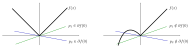
\includegraphics[width=1\textwidth]{./Figures/subdiferencial}
    \caption{Exemplo de subdiferencial.}
    \label{fig:subdiferencial}
\end{figure}

Agora podemos definir de forma rigorosa o fluxo de gradiente.

\begin{definition}[Fluxo de Gradiente]
    Seja $f:\mathbb R^n \to \mathbb R$.
    Dizemos que $x:(0,+\infty) \to \text{Dom}(f)$ é um fluxo de gradiente
    de $f$ se $x \in \text{AC}_{\text{loc}}((0,+\infty), \mathbb R^n)$ e
    \begin{equation}
        x'(t) \in - \nabla_G f(x(t)), \quad \text{para } \lambda\text{-a.e } t \in (0,+\infty),
    \end{equation}
    onde $\lambda$ é a medida de Lebesgue. Note que dizemos que $x$ começa em $x_0$ se
    $\lim_{t \to 0^+} x(t) = x_0$.
\end{definition}
\bibliography{ref}

\bibliographystyle{plainnat}

\newpage
\section{Appendix}

\subsection{Auxiliary - Probability and Analysis}
This section contains definitions and results in Probability and
Analysis that are used throughout the text. These results are listed
here mostly without proofs.

\begin{definition}
	Let $d:X\times X \to \mathbb R_+$. We say that $d$ is a metric on the set $X$ if
	for all $x,y,z \in X$, the following three assertions are true:
	\begin{enumerate}[i)]
		\item $d(x,y) = 0 \iff x = y$
		\item $d(x,y) = d(y,x)$
		\item $d(x,z) \leq d(x,y) + d(y,z)$ (triangle inequality)
	\end{enumerate}
	\label{def:metric}
\end{definition}

\begin{definition}(Weak convergence)
	We say that $\mu_n \rightharpoonup \mu$ if and only if
	$\forall f$ continuous and bounded, we have
	$\int f \ d\mu_n \to \int f \ d\mu$.
	\label{def:weakconv}
\end{definition}
Note that this is equivalent to the notion of convergence in distribution,
which is more commonly known in probability.

\begin{theorem}(Portmanteau)
	\label{Portmanteau}
	Given $\mu \in \mathcal{P}(X)$, where $X$ is a metric space.
	Then, the following statements are equivalent:
	\begin{enumerate}[i)]
		\item $\mu_n \rightharpoonup \mu$;

		\item $\forall f$ bounded and uniformly continuous,
		      we have $\int f \ d\mu_n \to \int f \ d\mu$;

		\item $\forall F \subset X$ closed,
		      $\mu(F) \geq \limsup_n \mu_n(F)$;

		\item $\forall F \subset X$ open,
		      $\mu(A) \leq \liminf_n \mu_n(A)$;

		\item $\forall B$ such that $\mu(\partial B)= 0$, then
		      $\mu_n(B) \to \mu(B)$.

		      Note that every set $B$ with
		      $\mu(\partial B)=0$is called
		      a continuity set. And $\partial B$ is the boundary set of
		      B, hence $\partial B := \hat B \setminus \mathring B$.
	\end{enumerate}

\end{theorem}

\begin{theorem}
	Let $X,Y$ be metric spaces and $\mu_n \rightharpoonup \mu$.
	Given a continuous map $h:X\to Y$, then
	$h_\# \mu_n = \mu_n \circ h^{-1} \rightharpoonup h_\# \mu$.
\end{theorem}

\begin{corollary}
	If $\mu_n \rightharpoonup \mu$ with $h:X\to Y$ such that
	$\mu(D_h) = 0$ where $D_h$ is the set of points of discontinuity.
	Then, $\mu_n \circ h^{-1}\rightharpoonup \mu \circ h^{-1}$.
\end{corollary}

\begin{proposition}
	If $X$ is Polish, and $d$ is a lower semi-continuous metric on $X$. For $p \in [1,+\infty)$ and $x_0 \in X$,
	$\mu_n \rightharpoonup \mu$ and $\int_X d(x,x_0)^p d\mu_n \to \int_X d(x,x_0)^p d \mu$, if, and only if,
	$\mu_n \rightharpoonup \mu$ and $\lim_{R \to \infty} \int_{d(x,x_0)\geq R} d(x,x_0) d\mu_n \to 0$ (uniformly integrable).
\end{proposition}

\begin{definition} (Tight)
	A family of probability measures $\mathcal{A}$ is tight if for
	$\epsilon > 0$, $\exists K \subset X$ compact, such that for
	any $\mu_\alpha \in \mathcal{A}$,
	$\mu_\alpha (X \setminus K)<\epsilon$
	\label{def:tight}
\end{definition}

\begin{theorem}(Prokhorov) This theorem
	consists in two separate results.
	\label{Prokhorov}
	\begin{enumerate}[i)]
		\item If the family $\mathcal{G} =
			      \{\mu_\alpha\}_{\alpha \in \Lambda}$ is tight, then
		      $\mathcal{G}$ is sequentially pre-compact, i.e. for any
		      $(\mu_n) \subset \mathcal{G}$,
		      $\exists \mu_{n_k}\rightharpoonup \mu$, where
		      $\mu \in \overline{\mathcal{G}}$;

		\item If X is Polish and $\mathcal{G}=
			      \{\mu_\alpha\}_{\alpha \in \Lambda}\subset \mathcal{P}(X)$
		      is pre-compact. Then $\mathcal{G}$ is tight.
		      In other words, for $X$ polish, and $\mu_n \in \mathcal{P}(X)$
		      with $\mu_n \rightharpoonup \mu$, then the sequence
		      $(\mu_n)$ is tight.
	\end{enumerate}
\end{theorem}

\begin{definition}(Disintegration)

	For a Borel measurable space $X$ with a measure $\mu$.
	Given a function $f:X \to Y$. We say that the family
	$(\mu_y)_{y\in Y}$ is a Disintegration of $\mu$ according
	to $f$ if every measure $\mu_y$ is concentrated on $f^{-1}(\{y\})$, and
	for every $\phi \in C(X)$, the map $\phi \mapsto \int_X \phi d \mu_y$ is
	Borel measurable with
	\begin{equation}
		\int_X \phi \ d\mu = \int_Y \int_X \phi \ d\mu_y (x) \ d\nu(y), \quad
		\text{ where } \nu = f_\# \mu
	\end{equation}
	Note that the existence and uniqueness of disintegration families depend on the
	spaces where the probabilities are defined, to which we introduce the next theorem.
	\label{def:disintegration}
\end{definition}

\begin{theorem}(\citet{garling2018analysis} 16.10.1)
	Suppose that $X$ and $Y$ are Polish spaces, that $\mu \in \mathcal P(X)$ and that
	$f$ is a Borel measurable map from $X$ to $Y$. Then, the $f$-disintegration
	of $\mu$ exists, and is essentially unique (i.e.
	$\mu(f^{-1}(B))=0$, with
	$B := \{y \in f(X) : \mu_y \neq \mu_y'\}$ where $\mu_y$ and $\mu_y'$ are two disintegrations).
	\label{thm:disintegrationunique}
\end{theorem}

\begin{theorem}
	$f:X \to \mathbb R$ is uniformly continuous $\iff$
	$\exists \ \omega : \mathbb R_+ \to \mathbb R_+$ , such that
	$\omega$ is increasing and $\lim_{x \to 0} w(x) = 0$ with
	$|f(x) - f(y)| \leq \omega(d(x,y)), \ \forall x,y \in X$.
	We call $\omega$ the modulus of continuity.
	\label{thm:mod_continuity}
\end{theorem}

\begin{definition}(Equicontinuous)
	For a metric space $X$, the sequence of functions
	$f_n:X\to \mathbb R$ is equicontinuous if
	$\forall \epsilon >0,\ \exists \delta >0: \ d(x,y) < \delta
		\implies d(f_n(x),f_n(y))<\epsilon$ for every $n \in \mathbb N$.
	\label{def:equicontinuous}
\end{definition}

\begin{definition}(Equibounded) We say that a sequence (or family)
	of functions $(f_n)$ is equibounded,
	if $\exists M > 0 \ : \ |f_n(x)|< M < +\infty \ \forall n \in
		\mathbb N$. In words, there is a value $M$ that bounds all functions
	in the sequence.
	\label{def:equibounded}
\end{definition}

\begin{theorem}(Arzelà-Ascoli)
	If $X$ is a compact metric space with $f_n$ equicontinuous and
	equibounded, then $\exists f_{n_k}\to_{\text{unif.}}f$, where
	$f$ is continuous.
	\label{thm:arzela-ascoli}
\end{theorem}

\begin{theorem}
	Let $(X,d)$ be metric space. Thus, if $X$ is compact, then $\mathrm{Lip}(X)$ is dense in $C(X)$.
	\label{thm:lipdense}
\end{theorem}
\begin{prf} (Proof from \citet{stackoverflow1})
	Let $g:X\to \mathbb R$ be a continuous function, then
	since $X$ is compact, $g$ is uniformly continuous.
	Therefore, for any $\varepsilon>0$, one can take a
	$\delta >0$ such that $d(x,y) < \delta$ implies
	$|g(x)-g(y)|<\varepsilon$. Now, let $M = \sup_{x}|g(x)|$
	and define
	\begin{equation*}
		f(x) :=
		\sup_y g(y) - \frac{2Md(x,y)}{\delta}
	\end{equation*}
	Now, note that $f$ is Lipschitz, since
	\begin{align*}
		f(x_1) - f(x_2) &= 
		\sup_y \left(g(y) - \frac{2Md(x_1,y)}{\delta}\right) -
		\sup_y \left(g(y) - \frac{2Md(x_2,y)}{\delta} \right)\\
		&\leq
		\sup_y \frac{2M(d(x_1,y)-d(x_2,y))}{\delta})
	\end{align*}
	By the triangle inequality, $d(x_1,y) - d(x_2,y) \leq d(x_1,x_2)$, then
	\begin{equation*}
		\sup_y \frac{2M(d(x_1,y)-d(x_2,y))}{\delta} \leq 
		\sup_y \frac{2Md(x_1,x_2)}{\delta} = 
		\frac{2Md(x_1,x_2)}{\delta}
	\end{equation*}
	The same argument is valid by exchanging $x_1$ and $x_2$, so $f$ has Lipschitz constant
	$\frac{2M}{\delta}$. Next, let's prove that $\sup_x |g(x) - f(x)| < \varepsilon$.

	A first point to notice is that $f(x)\geq g(x)$, since for $y=x$, we have $f(x) = g(x)$.
	For $d(x,y) \geq \delta$,
	\begin{equation*}
		f(x) = \sup_y g(y) - \frac{2M d(x,y)}{\delta}\leq \sup_y - 2M \leq -M \leq g(x)
	\end{equation*}
	Hence $f(x)\geq g(x) \geq f(x)$, so we obtain an equality.

	For $d(x,y) < \delta$,
	\begin{equation*}
		f(x) - g(x) = \sup_y g(y) - g(x) - \frac{2M d(x,y)}{\delta}
		\leq \varepsilon -\frac{2M d(x,y)}{\delta} < \varepsilon
	\end{equation*}
	We conclude that $0< f(x) - g(x) < \varepsilon$, so $\sup_x|f(x)-g(x)|< \varepsilon$.

\end{prf}


\subsection{Auxiliary - Inequalities}

\begin{lemma}(Inf-Sup Inequality)
	\begin{equation}
		|\inf_{x \in A} f(x) - \inf_{x \in A} g(x)| \leq
		\sup_{x \in A}|f(x)- g(x)|
	\end{equation}
	\label{lem:infsup_ineq}
\end{lemma}
\begin{prf}
	Let's write $\sup_{x \in A}f(x)$ as $\sup_A f$ for simplicity.
	Note that $f = f - g + g$, hence,
	\begin{align*}
		\sup_A f = \sup_A f - g + g & \leq
		\sup_A (f-g) + \sup_A g \implies   \\
		\sup_A f - \sup_A g         & \leq
		\sup_A f-g \leq \sup_A |f-g|       \\
	\end{align*}
	Using the same argument for $g$, we obtain that
	\begin{equation}
		|\sup_A f - \sup_A g| \leq \sup_A |f-g|
	\end{equation}

	Finally, note that
	\begin{align*}
		|\sup_A f - \sup_A g| =
		|\inf_A (-f) - \inf_A (-g)| & =
		|-\inf_A f + \inf_A g| =                                                \\
		                            & =|\inf_A f - \inf_A g | \leq \sup_A |f-g|
	\end{align*}
\end{prf}

\begin{lemma} (Minkowski's Inequality)
	Let $X$ be a measurable space, for $p \in [1,+\infty)$ and $f,g \in L^p(X)$. Therefore,
	\begin{equation}
		||f + g||_{L^p(X)} \leq
		||f||_{L^p(X)} + 
		||g||_{L^p(X)}
	\end{equation}
	Where $||f||_{L^p(X)}^p = \int_X |f|^p d\mu$.
	\label{lem:minkowski}
\end{lemma}

\end{document}